\documentclass[a4paper,adobefonts,11pt,UTF8]{book}

\usepackage{ctex}
\usepackage{makeidx}

%Bibliography
\usepackage{chapterbib}
\usepackage[sectionbib,square,super,sort&compress]{natbib}

\usepackage[headheight=13.6pt]{geometry}
\usepackage{fontspec}
\usepackage{xunicode}
\usepackage{xltxtra}
\usepackage{amsmath}
\usepackage{amssymb}
\usepackage{verbatim}
\usepackage{graphicx}


\graphicspath{{../img/}}

\usepackage{colortbl}
\usepackage[svgnames,table]{xcolor}
\usepackage{paralist}
\usepackage[figuresright]{rotating}
\usepackage{longtable}
\usepackage{array}
\usepackage{makecell}
\newcommand\mgape[1]{\gape{$\vcenter{\hbox{#1}}$}}
\usepackage{ulem}
%\usepackage{rotating}
\usepackage{color,colortbl}

\usepackage{tikz}

\usepackage{listings}
\lstset{
	basicstyle=\ttfamily,
	showstringspaces=false,
	commentstyle=\color{red},
	keywordstyle=\color{blue},
	columns=flexible
}

\usepackage{bashful}

\usepackage[bookmarksnumbered,pdfencoding=auto,pdfauthor={穷屌丝联盟},pdfpagelayout=TwoPageRight,breaklinks,colorlinks,linkcolor=RoyalBlue,urlcolor=blue,colorlinks=true]{hyperref}

\usepackage{fancyhdr}

\pagestyle{fancy}
\fancyhf{}
\fancyhead[LE,RO]{\thepage}
\fancyhead[RE]{\leftmark}
\fancyhead[RO]{\rightmark}
\fancypagestyle{plain}{
	\fancyhf{}
	\renewcommand{\headrulewidth}{0pt}
}

%titlepage \titleGM
\newcommand*{\plogo}{\fbox{$\mathcal{PL}$}} % Generic publisher logo

%----------------------------------------------------------------------------------------
%	TITLE PAGE
%----------------------------------------------------------------------------------------

\newcommand*{\titleGM}{\begingroup % Create the command for including the title page in the document
\hbox{ % Horizontal box
\hspace*{0.2\textwidth} % Whitespace to the left of the title page
\rule{1pt}{\textheight} % Vertical line
\hspace*{0.05\textwidth} % Whitespace between the vertical line and title page text
\parbox[b]{0.75\textwidth}{ % Paragraph box which restricts text to less than the width of the page

{\noindent\Huge\bfseries Notes Collection of \\[0.5\baselineskip] JavaScript}\\[2\baselineskip] % Title
{\large \textit{JavaScript}}\\[4\baselineskip] % Tagline or further description
{\Large \textsc{theqiong.com}} % Author name

\vspace{0.5\textheight} % Whitespace between the title block and the publisher
{\noindent 穷屌丝联盟 }\\[\baselineskip] % Publisher and logo
}}
\endgroup}
%

%lstlisting[language=JavsScript]
% Taken from Lena Herrmann at 
% http://lenaherrmann.net/2010/05/20/javascript-syntax-highlighting-in-the-latex-listings-package
\definecolor{lightgray}{rgb}{.9,.9,.9}
\definecolor{darkgray}{rgb}{.4,.4,.4}
\definecolor{purple}{rgb}{0.65, 0.12, 0.82}

\lstdefinelanguage{javascript}{
  keywords={typeof, new, true, false, catch, function, return, null, catch, switch, var, if, in, while, do, else, case, break},
  keywordstyle=\color{blue}\bfseries,
  ndkeywords={class, export, boolean, throw, implements, import, this},
  ndkeywordstyle=\color{darkgray}\bfseries,
  identifierstyle=\color{black},
  sensitive=false,
  comment=[l]{//},
  morecomment=[s]{/*}{*/},
  commentstyle=\color{purple}\ttfamily,
  stringstyle=\color{red}\ttfamily,
  morestring=[b]',
  morestring=[b]"
}

\lstset{
   language=javascript,
   backgroundcolor=\color{lightgray},
   extendedchars=true,
   basicstyle=\footnotesize\ttfamily,
   showstringspaces=false,
   showspaces=false,
   numbers=left,
   numberstyle=\footnotesize,
   numbersep=9pt,
   tabsize=2,
   breaklines=true,
   showtabs=false,
   captionpos=b
}
%

\lstdefinelanguage{Scheme}
{morekeywords={,lambda, cond, case, display, let, import, quote, quasiquote, unquote,
define, begin, newline, if, list, apply, null?, car, cdr, or, not, and, for-each, 
make-vector, vector-length, vector-ref, vector-set!, eqv?, eq?, equal?, else, set!, 
define-record-type, fields, mutable, immutable, assert, parent, with-exception-handler, }
sensitive=false,
morecomment=[l]{;},
morecomment=[s]{/*}{*/},
morestring=[b]",
}

\lstdefinelanguage{CSS}{
  morekeywords={accelerator,azimuth,background,background-attachment,
    background-color,background-image,background-position,
    background-position-x,background-position-y,background-repeat,
    behavior,border,border-bottom,border-bottom-color,
    border-bottom-style,border-bottom-width,border-collapse,
    border-color,border-left,border-left-color,border-left-style,
    border-left-width,border-right,border-right-color,
    border-right-style,border-right-width,border-spacing,
    border-style,border-top,border-top-color,border-top-style,
    border-top-width,border-width,bottom,caption-side,clear,
    clip,color,content,counter-increment,counter-reset,cue,
    cue-after,cue-before,cursor,direction,display,elevation,
    empty-cells,filter,float,font,font-family,font-size,
    font-size-adjust,font-stretch,font-style,font-variant,
    font-weight,height,ime-mode,include-source,
    layer-background-color,layer-background-image,layout-flow,
    layout-grid,layout-grid-char,layout-grid-char-spacing,
    layout-grid-line,layout-grid-mode,layout-grid-type,left,
    letter-spacing,line-break,line-height,list-style,
    list-style-image,list-style-position,list-style-type,margin,
    margin-bottom,margin-left,margin-right,margin-top,
    marker-offset,marks,max-height,max-width,min-height,
    min-width,-moz-binding,-moz-border-radius,
    -moz-border-radius-topleft,-moz-border-radius-topright,
    -moz-border-radius-bottomright,-moz-border-radius-bottomleft,
    -moz-border-top-colors,-moz-border-right-colors,
    -moz-border-bottom-colors,-moz-border-left-colors,-moz-opacity,
    -moz-outline,-moz-outline-color,-moz-outline-style,
    -moz-outline-width,-moz-user-focus,-moz-user-input,
    -moz-user-modify,-moz-user-select,orphans,outline,
    outline-color,outline-style,outline-width,overflow,
    overflow-X,overflow-Y,padding,padding-bottom,padding-left,
    padding-right,padding-top,page,page-break-after,
    page-break-before,page-break-inside,pause,pause-after,
    pause-before,pitch,pitch-range,play-during,position,quotes,
    -replace,richness,right,ruby-align,ruby-overhang,
    ruby-position,-set-link-source,size,speak,speak-header,
    speak-numeral,speak-punctuation,speech-rate,stress,
    scrollbar-arrow-color,scrollbar-base-color,
    scrollbar-dark-shadow-color,scrollbar-face-color,
    scrollbar-highlight-color,scrollbar-shadow-color,
    scrollbar-3d-light-color,scrollbar-track-color,table-layout,
    text-align,text-align-last,text-decoration,text-indent,
    text-justify,text-overflow,text-shadow,text-transform,
    text-autospace,text-kashida-space,text-underline-position,top,
    unicode-bidi,-use-link-source,vertical-align,visibility,
    voice-family,volume,white-space,widows,width,word-break,
    word-spacing,word-wrap,writing-mode,z-index,zoom},
  morestring=[s]{:}{;},
  sensitive,
  morecomment=[s]{/*}{*/}
}

\setmainfont[Mapping=tex-text]{Minion Pro}

\makeindex


\title{JavaScript Notes}
\author{穷屌丝联盟}
\date{\today}

\begin{document}

\begin{titlepage}
\addcontentsline{toc}{part}{Cover}

\pagestyle{empty} % Removes page numbers

\titleGM % This command includes the title page


\end{titlepage}


\maketitle
\tableofcontents
\listoffigures
\listoftables
\printindex



\part{Introduction}

JavaScript (JS)\cite{javascript} is an interpreted computer programming language. As part of web browsers, implementations allow client-side scripts to interact with the user, control the browser, communicate asynchronously, and alter the document content that is displayed. It has also become common in server-side programming, game development and the creation of desktop applications.


JavaScript is a prototype-based scripting language with dynamic typing and has first-class functions. Its syntax was influenced by C. JavaScript copies many names and naming conventions from Java, but the two languages are otherwise unrelated and have very different semantics. The key design principles within JavaScript are taken from the Self and Scheme programming languages. It is a multi-paradigm language, supporting object-oriented, imperative, and functional programming styles.


The application of JavaScript to uses outside of web pages~—~for example, in PDF documents, site-specific browsers, and desktop widgets~—~is also significant. Newer and faster JavaScript VMs and frameworks built upon them (notably Node.js) have also increased the popularity of JavaScript for server-side web applications.

JavaScript was formalized in the ECMAScript language standard and is primarily used as part of a web browser (client-side JavaScript). This enables programmatic access to computational objects within a host environment.

JavaScript是一种动态类型、弱类型、基于原型的语言,JavaScript不仅是直译式脚本语言,而且内置支持类型,它的解释器(被称为JavaScript引擎)也是浏览器的一部份。



JavaScript最早是在HTML网页上使用,用来给HTML网页增加动态功能,比如JavaScript 常用于验证用户的输入,比如在下面的例子中,如果输入值不是数字,浏览器会弹出提示框。



\begin{lstlisting}[language=HTML]
<input id="demo" type="text">

<script>
function myFunction()
{
var x=document.getElementById("demo").value;
if(x==""||isNaN(x))
	{
	alert("Not Numeric");
	}
}
</script>

<button type="button" onclick="myFunction()">点击这里</button>
\end{lstlisting}

不同于服务器端脚本语言,例如PHP与ASP,JavaScript主要被作为客户端脚本语言在用户的浏览器上运行,不需要服务器的支持,所以在早期程序员比较青睐于JavaScript以减少对服务器的负担,而与此同时也带来另一个问题:安全性。


然而现在随着服务器的强壮,虽然现在的程序员更喜欢运行于服务端的脚本以保证安全,但JavaScript仍然以其跨平台、容易上手等优势被应用于不同的接口上,而且JavaScript也开始被用于网络服务器,如Node.js。

有些特殊功能(如AJAX)必须依赖Javascript在客户端进行支持。随着引擎如V8和框架如Node.js的发展,及其事件驱动及异步IO等特性,JavaScript逐渐被用来编写服务器端程序。



\chapter{Histroy}

JavaScript was originally developed by Brendan Eich. While battling with Microsoft over the Web, Netscape considered their client-server offering a distributed OS, running a portable version of Sun Microsystems' Java. Because Java was a competitor of C++ and aimed at professional programmers, Netscape also wanted a lightweight interpreted language that would complement Java by appealing to nonprofessional programmers, like Microsoft's Visual Basic.

Although it was developed under the name Mocha, the language was officially called LiveScript when it first shipped in beta releases of Netscape Navigator 2.0 in September 1995, but it was renamed JavaScript when it was deployed in the Netscape browser version 2.0B3.


The change of name from LiveScript to JavaScript roughly coincided with Netscape adding support for Java technology in its Netscape Navigator web browser. The final choice of name caused confusion, giving the impression that the language was a spin-off of the Java programming language, and the choice has been characterized by many as a marketing ploy by Netscape to give JavaScript the cachet of what was then the hot new web programming language.

Netscape introduced an implementation of the language for server-side scripting (SSJS) with Netscape Enterprise Server, first released in December, 1994 (soon after releasing JavaScript for browsers). Since the mid-2000s, there has been a proliferation of server-side JavaScript implementations. Node.js is one recent notable example of server-side JavaScript being used in real-world applications.


JavaScript very quickly gained widespread success as a client-side scripting language for web pages. Microsoft introduced JavaScript support in its own web browser, Internet Explorer, in version 3.0, released in August 1996. Microsoft's webserver, Internet Information Server, introduced support for server-side scripting in JavaScript with release 3.0 (1996). Microsoft started to promote webpage scripting using the umbrella term Dynamic HTML.



Microsoft's JavaScript implementation was later renamed JScript to avoid trademark issues. JScript added new date methods to fix the Y2K-problematic\footnote{Y2K问题则是直接与Java有关。\newline 根据设想,\textsf{Date.getYear()}返回的应该是年份的最后两位,但是实际上,对于2000年,它返回的是100。如果用这个函数生成年份,某些网页可能出现``19100"这样的结果。\newline 这个问题完全来源于Java,因为Javascript的日期类直接采用了\textcolor{Blue}{\texttt{java.util.Date}}函数库。Brendan Eich显然很不满意这个结果,这导致后来不得不添加了一个返回四位数年份的\textsf{Date.getFullYear()}函数。} methods in JavaScript, which were based on Java's \textcolor{Blue}{\texttt{java.util.Date}} class.


In November 1996, Netscape announced that it had submitted JavaScript to Ecma International for consideration as an industry standard, and subsequent work resulted in the standardized version named ECMAScript. In June 1997, Ecma International published the first edition of the ECMA-262 specification. A year later, in June 1998, some modifications were made to adapt it to the ISO/IEC-16262 standard, and the second edition was released. The third edition of ECMA-262 (published on December 1999) is the version most browsers currently use.

A fourth edition of the ECMAScript standard was not released and does not exist. Fifth edition of the Ecmascript standard was released in December 2009. The current edition of the ECMAScript standard is 5.1, released in June 2011.

JavaScript has become one of the most popular programming languages on the web. Initially, however, many professional programmers denigrated the language because its target audience consisted of web authors and other such "amateurs", among other reasons. The advent of Ajax returned JavaScript to the spotlight and brought more professional programming attention. The result was a proliferation of comprehensive frameworks and libraries, improved JavaScript programming practices, and increased usage of JavaScript outside of web browsers, as seen by the proliferation of server-side JavaScript platforms.


In January 2009, the CommonJS project was founded with the goal of specifying a common standard library mainly for JavaScript development outside the browser.

CommonJS is a project with the goal of specifying an ecosystem for JavaScript outside the browser (for example, on the server or for native desktop applications). The project was started by Kevin Dangoor in January 2009 and initially named ServerJS.

In August 2009, the project was renamed CommonJS to show the broader applicability of the APIs. Specifications are created and approved in an open process. A specification is only considered final after it has been finished by multiple implementations. CommonJS is not affiliated with the Ecma International group TC39 working on ECMAScript, but some members of TC39 participate in the project.

Today, ``JavaScript" is a trademark of Oracle Corporation. It is used under license for technology invented and implemented by Netscape Communications and current entities such as the Mozilla Foundation.

大概在 1992 年,一家称作 Nombas 的公司开发了一种叫做 C 减减(C-minus-minus,简称 Cmm)的嵌入式脚本语言。Cmm 背后的理念很简单:一个足够强大可以替代宏操作(macro)的脚本语言,同时保持与 C (和 C ++)足够的相似性,以便开发人员能很快学会。这个脚本语言捆绑在一个叫做 CEnvi 的共享软件中,它首次向开发人员展示了这种语言的威力。

Nombas 最终把 Cmm 的名字改成了 ScriptEase\footnote{原因是后面的部分(mm)听起来过于消极,同时字母 C “令人害怕”。},现在 ScriptEase 已经成为了 Nombas 产品背后的主要驱动力。

当 Netscape Navigator 崭露头角时,Nombas 开发了一个可以嵌入网页中的 CEnvi 的版本。这些早期的试验被称为 Espresso Page(浓咖啡般的页面),它们代表了第一个在万维网上使用的客户端语言。而 Nombas 丝毫没有料到它的理念将会成为万维网的一块重要基石。

当网上冲浪越来越流行时,对于开发客户端脚本的需求也逐渐增大。此时,大部分因特网用户还仅仅通过 28.8 kbit/s 的调制解调器连接到网络,即便这时网页已经不断地变得更大和更复杂。而更加加剧用户痛苦的是,仅仅为了简单的表单有效性验证,就要与服务器进行多次地往返交互。设想一下,用户填完一个表单,点击提交按钮,等待了 30 秒的处理后,看到的却是一条告诉你忘记填写一个必要的字段。

那时正处于技术革新最前沿的 Netscape,开始认真考虑开发一种客户端脚本语言来解决简单的处理问题。

当时工作于 Netscape 的 Brendan Eich,开始着手为即将在 1995 年发行的 Netscape Navigator 2.0 开发一个称之为 LiveScript\footnote{Netscape 与 Sun 及时完成了LiveScript 实现。}的脚本语言,当时的目的是在浏览器和服务器(本来要叫它 LiveWire)端使用它,而且就在 Netscape Navigator 2.0 即将正式发布前,Netscape 将其更名为 JavaScript,目的是为了利用 Java 这个因特网时髦词汇。Netscape 的赌注最终得到回报,JavaScript 从此变成了因特网的必备组件。

在1995年时,JavaScript由Netscape公司的布兰登·艾克,在Netscape浏览器上首次设计实现。因为Netscape公司与Sun公司合作,Netscape公司管理层次结构希望它外观看起来像Java,因此取名为JavaScript,但实际上它的语法风格与Self及Scheme较为接近\footnote{Netscape在最初将其脚本语言命名为LiveScript,后来Netscape在与Sun合作之后将其改名为JavaScript。JavaScript最初受Java启发而开始设计的,目的之一就是“看上去像Java”,因此语法上有类似之处,一些名称和命名规范也借自Java,但JavaScript的主要设计原则源自Self和Scheme。JavaScript与Java名称上的近似,是当时Netscape为了营销考虑与Sun Microsystem达成协议的结果。}。

因为 JavaScript 1.0 如此成功,Netscape 在 Netscape Navigator 3.0 中发布了 1.1 版。恰巧那个时候,微软决定进军浏览器,发布了 IE 3.0 并搭载了一个 JavaScript 的克隆版,叫做 JScript(这样命名是为了避免与 Netscape 潜在的许可纠纷)。微软步入 Web 浏览器领域的这重要一步虽然令其声名狼藉,但也成为 JavaScript 语言发展过程中的重要一步。

在微软进入后,有 3 种不同的 JavaScript 版本同时存在:Netscape Navigator 3.0 中的 JavaScript、IE 中的 JScript以及CEnvi推出的ScriptEase,它们与JavaScript同样都可在浏览器上运行,因此在JavaScript的标准并未确定时,同期有Netscape的JavaScript,微软的JScript和CEnvi的ScriptEase三足鼎立。

与 C 和其他编程语言不同的是,JavaScript 并没有一个标准来统一其语法或特性,而这 3 种不同的版本恰恰突出了这个问题。随着业界担心的增加,这个语言的标准化显然已经势在必行。

\chapter{ECMAScript}

1997 年,JavaScript 1.1 作为一个草案提交给欧洲计算机制造商协会(ECMA)。第 39 技术委员会(TC39)被委派来“标准化一个通用、跨平台、中立于厂商的脚本语言的语法和语义”(\url{http://www.ecma-international.org/memento/TC39.htm})。

为了统一规格,1997年,在ECMA(欧洲计算机制造商协会)的协调下,由来自Netscape、Sun、微软、Borland和其他一些对脚本编程感兴趣的公司的程序员组成的 TC39组成的工作组确定了统一标准:ECMA-262。

ECMA-262标准定义了名为 ECMAScript 的全新脚本语言。因为JavaScript兼容于ECMA标准,因此也称为ECMAScript,符合ECMA-262 3rd Edition标准的实现包括:

\begin{compactitem}
\item Microsoft公司的JScript
\item Mozilla的JavaScript-C(C语言实现),现名SpiderMonkey
\item Mozilla的Rhino(Java实现)
\item Digital Mars公司的DMDScript
\item Google公司的V8
\item WebKit
\end{compactitem}


在接下来的几年里,国际标准化组织及国际电工委员会(ISO/IEC)也采纳 ECMAScript 作为标准(ISO/IEC-16262)。从此,Web 浏览器就开始努力(虽然有着不同的程度的成功和失败)将 ECMAScript 作为 JavaScript 实现的基础。

ECMAScript 分成几个不同的版本,它是在ECMA-262 的标准中定义的。和其他标准一样,ECMA-262 会被编辑和更新。当有了主要更新时,就会发布一个标准的新版。最新 ECMA-262 的版本是 5.1,于 2011 年 6 月发布。


ECMA-262 的第一版在本质上与 Netscape 的 JavaScript 1.1 是一样,只是把所有与浏览器相关的代码删除了,此外还有一些小的调整。首先,ECMA-262 要求对 Unicode 标准的支持(以便支持多语言)。第二,它要求对象是平台无关的(Netscape 的 JavaScript 1.1 事实上有不同的对象实现,例如 Date 对象,是依赖于平台)。这是 JavaScript 1.1 和 1.2 为什么不符合 ECMA-262 规范第一版的主要原因。

ECMA-262 的第二版大部分更新本质上是编辑性的。这次标准的更新是为了与 ISO/IEC-16262 的严格一致,也并没有特别添加、更改和删除内容。ECMAScript 一般不会遵守第二版。

ECMA-262 第三版是该标准第一次真正的更新。它提供了对字符串处理、错误定义和数值输出的更新。同时,它还增加了正则表达式、新的控制语句、try...catch 异常处理的支持,以及一些为使标准国际化而做的小改动。一般来说,它标志着 ECMAScript 成为一种真正的编程语言。

\begin{longtable}{|m{45pt}|m{220pt}|m{100pt}|}
%head
\multicolumn{3}{r}{}
\tabularnewline\hline
版本	&说明	&实现
\endhead
%endhead

%firsthead
\caption{ECMA}\\
\hline
版本	&说明	&实现
\endfirsthead
%endhead

%foot
\multicolumn{3}{r}{}
\endfoot
%endfoot

%lastfoot
\endlastfoot
%endlastfoot
\hline
ECMA v1	&标准化了JavaScript1.1的基本特性,并添加了一些新特性。没有标准化switch语句和正则表达式。	&由Netscape 4.5和IE 4实现。\\
\hline
ECMA v2	&ECMA v1的维护版本,只添加了说明。															&由Netscape 4.5和IE 4实现。\\
\hline
ECMA v3	&标准化了switch语句、异常处理和正则表达式。													&由Mozilla、Netscape 6和IE 5.5实现。\\
\hline
\end{longtable}






含有 JavaScript 1.1 的 Netscape Navigator 3.0 在 1996 年发布。然后,JavaScript 1.1 规范被作为一个新标准的草案被提交给 EMCA。有了 JavaScript 轰动性的流行,Netscape 十分高兴地开始开发 1.2 版。但有一个问题,ECMA 并未接受 Netscape 的草案。在 Netscape Navigator 3.0 发布后不久,微软就发布了 IE 3.0。该版本的 IE 含有 JScript 1.0(微软自己的 JavaScript 实现的名称),原本计划可以与 JavaScript 1.1 相提并论。然后,由于文档不全以及一些不当的重复特性,JScript 1.0 远远没有达到 JavaScript 1.1 的水平。

在 ECMA-262 第一版定稿之前,发布含有 JavaScript 1.2 的 Netscape Navigator 4.0 是在 1997 年,在那年晚些时候,ECMA-262 标准被接受并标准化。因此,JavaScript 1.2 并不和 ECMAScript 的第一版兼容,虽然 ECMAScript 应该基于 JavaScript 1.1。

JScript 的下一步是 IE 4.0 中加入的 JScript 3.0(2.0 版是随 IIS 3.0 一起发布的,但并未包含在浏览器中)。微软大力宣传 JScript 3.0 是世界上第一个真正符合 ECMA 标准的脚本语言。而那时,ECMA-262 还没有最终定稿,所以 JScript 3.0 也遭受了和 JavaScript 1.2 同样的命运 - 它还是没能符合最终的 ECMAScript 标准。

Netscape 选择在 Netscape Navigator 4.06 中升级它的 JavaScript 实现。JavaScript 1.3 使 Netscape 终于完全符合了 ECMAScript 第一版。Netscape 加入了对 Unicode 标准的支持,并让所有的对象保留了在 JavaScript 1.2 中引入的新特性的同时实现了平台独立。

当 Netscape 将它的源代码作为 Mozilla 项目公布于众时,本来计划 JavaScript 1.4 将会嵌入到 Netscape Navigator 5.0 中。然而,一个冒进的决定——要完全从头重新设计 Netscape 的代码,破坏了这个工作。JavaScript 1.4 仅仅作为一个 Netscape Enterprise Server 的服务器端脚本语言发布,以后也没有被放入浏览器中。

如今,所有主流的 Web 浏览器都遵守 ECMA-262 第三版。下面的表格列出了大部分流行的 Web 浏览器中的 ECMAScript 支持:

\begin{longtable}{|m{150pt}|m{150pt}|}
%head
\multicolumn{2}{r}{}
\tabularnewline\hline
浏览器	&DOM 兼容性
\endhead
%endhead

%firsthead
\hline
浏览器	&DOM 兼容性
\endfirsthead
%endfirsthead

%foot
\multicolumn{2}{r}{}
\endfoot
%endfoot

%lastfoot
\endlastfoot
%endlastfoot

\hline
Netscape Navigator 2.0			&-\\
\hline
Netscape Navigator 3.0			&-\\
\hline
Netscape Navigator 4.0 - 4.05	&-\\
\hline
Netscape Navigator 4.06 - 4.79	&Edition 1\\
\hline
Netscape 6.0+ (Mozilla 0.6.0+)	&Edition 3\\
\hline
Internet Explorer 3.0			&-\\
\hline
Internet Explorer 4.0			&-\\
\hline
Internet Explorer 5.0			&Edition 1\\
\hline
Internet Explorer 5.5+			&Edition 3\\
\hline
Opera 6.0 - 7.1					&Edition 2\\
\hline
Opera 7.2+						&Edition 3\\
\hline
Safari 1.0+/Konqueror~2.0+	&Edition 3\\
\hline
\end{longtable}

\chapter{DOM}



自从 IE 4.0 和 Netscape Navigator 4.0 开始支持不同形态的动态 HTML(DHTML),开发者首次能够在不重载网页的情况下修改它的外观和内容。这是 Web 技术的一大飞跃,不过也带来了巨大的问题。Netscape 和微软各自开发自己的 DHTML,从而结束了 Web 开发者只编写一个 HTML 页面就可以在所有浏览器中访问的时期。

业界决定必须要做点什么以保持 Web 的跨平台特性,他们担心如果放任 Netscape 和微软公司这样做,Web 必将分化为两个独立的部分,每一部分只适用于特定的浏览器。因此,负责指定 Web 通信标准的团体 W3C(World Wide Web Consortium)就开始制定 DOM\footnote{注意,DOM 不是 JavaScript 专有的,事实上许多其他语言都实现了它。不过,Web 浏览器中的 DOM 已经用 ECMAScript 实现了,现在是 JavaScript 语言的一个很大组成部分。}。

DOM(文档对象模型)是 HTML 和 XML 的应用程序接口(API)。DOM 将把整个页面规划成由节点层级构成的文档。HTML 或 XML 页面的每个部分都是一个节点的衍生物。考虑下面的 HTML 页面:


\begin{lstlisting}[language=HTML]
<html>
  <head>
    <title>Sample Page</title>
  </head>
  <body>
    <p>hello world!</p>
  </body>
</html>
\end{lstlisting}

这段代码可以用 DOM 绘制成一个节点层次图:


\begin{figure}[!h]
\centering
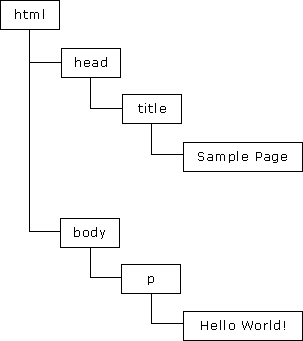
\includegraphics[scale=0.5]{js_dom.png}
\vspace{-10pt}
\caption{DOM节点层次图}
\label{js_dom}
\end{figure}

DOM 通过创建树来表示文档,从而使开发者对文档的内容和结构具有空前的控制力,使用 DOM API 可以轻松地删除、添加和替换节点。

DOM Level 1 是 W3C 于 1998 年 10 月提出的,它由两个模块组成,即 DOM Core 和 DOM HTML。前者提供了基于 XML 的文档的结构图,以便访问和操作文档的任意部分;后者添加了一些 HTML 专用的对象和方法,从而扩展了 DOM Core。

DOM Level 1 只是一个目标,即规划文档的结构,DOM Level 2 的目标就广泛多了。对原始 DOM 的扩展添加了对鼠标和用户界面事件(DHTML 对此有丰富的支持)、范围、遍历(重复执行 DOM 文档的方法)的支持,并通过对象接口添加了对 CSS(层叠样式表)的支持。由 Level 1 引入的原始 DOM Core 也加入了对 XML 命名空间的支持。

DOM Level 2 引入了几种 DOM 新模块,用于处理新的接口类型:

\begin{compactitem}
\item DOM 视图 - 描述跟踪文档的各种视图(即 CSS 样式化之前和 CSS 样式化之后的文档)
\item DOM 事件 - 描述事件的接口
\item DOM 样式 - 描述处理基于 CSS 样式的接口
\item DOM 遍历和范围 - 描述遍历和操作文档树的接口
\end{compactitem}

DOM Level 3 引入了以统一的方式载入和保持文档的方法(包含在新模块 DOM Load and Save)以及验证文档(DOM Validation)的方法,从而进一步扩展了 DOM。在 Level 3 中,DOM Core 被扩展为支持所有的 XML 1.0 特性,包括 XML Infoset、XPath 和 XML Base。

注意,根本没有 DOM Level 0 这个标准,它只是 DOM 的一个历史参考点(DOM Level 0 指的是 IE 4.0 和 Netscape Navigator 4.0 中支持的原始 DHTML)。

除了 DOM Core 和 DOM HTML 外,还有其他几种语言发布了自己的 DOM 标准。这些语言都是基于 XML 的,每种 DOM 都给对应语言添加了特有的方法和接口:

\begin{compactitem}
\item 可缩放矢量语言(SVG)1.0
\item 数字标记语言(MathML)1.0
\item 同步多媒体集成语言(SMIL)
\end{compactitem}

此外,其他语言也开发了自己的 DOM 实现,如 Mozilla 的 XML 用户界面语言(XUL)。不过,只有上面列出的几种语言是 W3C 的推荐标准。

DOM 在被 Web 浏览器开始实现之前就已经是一种标准了。IE 首次尝试 DOM 是在 5.0 版本中,不过其实直到 5.5 版本之后才具有真正的 DOM 支持,IE 5.5 实现了 DOM Level 1。从那时起,IE 就没有引入新的 DOM 功能。

Netscape 直到 Netscape 6(Mozilla 0.6.0)才引入 DOM 支持。目前,Mozilla 具有最好的 DOM 支持,实现了完整的 Level 1、几乎所有 Level 2 以及一部分 Level 3。(Mozilla 开发小组的目标是构造一个与标准 100\% 兼容的浏览器,他们的工作得到了回报。)

Opera 直到 7.0 版本才加入 DOM 支持,还有 Safari 也实现了大部分 DOM Level 1。它们几乎都与 IE 5.5 处于同一水平,有些情况下,甚至超过了 IE 5.5。不过,就对 DOM 的支持而论,所有浏览器都远远落后于 Mozilla。下表列出了常用浏览器对 DOM 的支持。

\begin{longtable}{|m{150pt}|m{180pt}|}
%head
\multicolumn{2}{r}{}
\tabularnewline\hline
浏览器	&DOM 兼容性
\endhead
%endhead

%firsthead
\hline
浏览器	&DOM 兼容性
\endfirsthead
%endfirsthead

%foot
\multicolumn{2}{r}{}
\endfoot
%endfoot

%lastfoot
\endlastfoot
%endlastfoot

\hline
Netscape Navigator 1.0 - 4.x			&-\\
\hline
Netscape 6.0+ (Mozilla 0.6.0+)			&Level 1、Level 2、Level 3(部分)\\
\hline
IE 2.0 - 4.x								&-\\
\hline
IE 5.0									&Level 1(最小)\\
\hline
IE 5.5+									&Level 1(几乎全部)\\
\hline
Opera 1.0 - 6.0							&-\\
\hline
Opera 7.0+								&Level 1(几乎全部)、Level 2 (部分)\\
\hline
Safari 1.0+/Konqueror ~ 2.0+			&Level 1\\
\hline
\end{longtable}


\chapter{BOM}

IE 3.0 和 Netscape Navigator 3.0 提供了一种特性 - BOM(浏览器对象模型),可以对浏览器窗口进行访问和操作。使用 BOM,开发者可以移动窗口、改变状态栏中的文本以及执行其他与页面内容不直接相关的动作。使 BOM 独树一帜且又常常令人怀疑的地方在于,它只是 JavaScript 的一个部分,没有任何相关的标准。

BOM 主要处理浏览器窗口和框架,不过通常浏览器特定的 JavaScript 扩展都被看做 BOM 的一部分。这些扩展包括:

\begin{compactitem}
\item 弹出新的浏览器窗口
\item 移动、关闭浏览器窗口以及调整窗口大小
\item 提供 Web 浏览器详细信息的定位对象
\item 提供用户屏幕分辨率详细信息的屏幕对象
\item 对 cookie 的支持
\item IE 扩展了 BOM,加入了 ActiveXObject 类,可以通过 JavaScript 实例化 ActiveX 对象
\end{compactitem}

由于没有相关的 BOM 标准,每种浏览器都有自己的 BOM 实现。有一些事实上的标准,如具有一个窗口对象和一个导航对象,不过每种浏览器可以为这些对象或其他对象定义自己的属性和方法。



\chapter{Validation}



\section{Form validation}

JavaScript 可用来在数据被送往服务器前对 HTML 表单中的这些输入数据进行验证。

被 JavaScript 验证的这些典型的表单数据有:

\begin{compactitem}
\item 用户是否已填写表单中的必填项目?
\item 用户输入的邮件地址是否合法?
\item 用户是否已输入合法的日期?
\item 用户是否在数据域 (numeric field) 中输入了文本?
\end{compactitem}

下面的函数用来检查用户是否已填写表单中的必填(或必选)项目。假如必填或必选项为空,那么警告框会弹出,并且函数的返回值为 false,否则函数的返回值则为 true(意味着数据没有问题):

\begin{lstlisting}[language=JavaScript]
function validate_required(field,alerttxt){
  with (field)
  {
    if (value==null||value==""){
      alert(alerttxt);
      return false;
    }
    else {
      return true;
    }
  }
}
\end{lstlisting}

下面是连同 HTML 表单的代码:


\begin{lstlisting}[language=HTML]
<html>
<head>
<script type="text/javascript">

function validate_required(field,alerttxt)
{
with (field)
  {
  if (value==null||value=="")
    {alert(alerttxt);return false}
  else {return true}
  }
}

function validate_form(thisform)
{
with (thisform)
  {
  if (validate_required(email,"Email must be filled out!")==false)
    {email.focus();return false}
  }
}
</script>
</head>

<body>
<form action="submitpage.htm" onsubmit="return validate_form(this)" method="post">
Email: <input type="text" name="email" size="30">
<input type="submit" value="Submit"> 
</form>
</body>

</html>
\end{lstlisting}

\section{Email validation}


下面的函数检查输入的数据是否符合电子邮件地址的基本语法。

这里要验证的是,输入的数据必须包含 @ 符号和点号(.)。同时,@ 不可以是邮件地址的首字符,并且 @ 之后需有至少一个点号:

\begin{lstlisting}[language=JavaScript]
function validate_email(field,alerttxt){
  with (field)
  {
    apos=value.indexOf("@")
    dotpos=value.lastIndexOf(".")
    if (apos<1||dotpos-apos<2){
      alert(alerttxt);return false
    }
    else {
      return true
    }
  }
}
\end{lstlisting}

下面是连同 HTML 表单的完整代码:

\begin{lstlisting}[language=HTML]
<html>
<head>
<script type="text/javascript">
function validate_email(field,alerttxt){
  with (field){
    apos=value.indexOf("@")
    dotpos=value.lastIndexOf(".")
    if (apos<1||dotpos-apos<2){
      alert(alerttxt); 
      return false;
    }
    else {
      return true;
    }
  }
}

function validate_form(thisform){
  with (thisform){
    if (validate_email(email,"Not a valid e-mail address!")==false){
      email.focus();
      return false;
    }
  }
}
</script>
</head>

<body>
<form action="submitpage.htm"onsubmit="return validate_form(this);" method="post">
Email: <input type="text" name="email" size="30">
<input type="submit" value="Submit"> 
</form>
</body>

</html>
\end{lstlisting}

\chapter{Features}

Javascript被归类为直译语言,因为目前主流的引擎都是每次运行时加载代码并解译。V8是将所有代码解译后再开始运行,其他引擎则是逐行解译(SpiderMonkey会将解译过的指令暂存,以提高性能,称为实时编译),但由于V8的核心部份多数用Javascript撰写(而SpiderMonkey是用C++),因此在不同的测试上,两者性能互有优劣。

JavaScript作为一种脚本语言,其源代码在发往客户端运行之前不需经过编译,而是将文本格式的字符代码发送给浏览器由浏览器解释运行。直译语言的弱点是安全性较差,而且在JavaScript中,如果一条运行不了,那么下面的语言也无法运行。而其解决办法就是于使用~\textcolor{Blue}{\texttt{try\{\}...catch()\{\}}}︰

\begin{lstlisting}[language=JavaScript]
console.log("a");    //这是正确的
console.log("b");    //这是正确的
console.logg("c");   //这是错误的,并且到这里会停下来
console.log("d");    //这是正确的
console.log("e");    //这是正确的
 
/*解决办法*/
try{console.log("a");}catch(e){}    //这是正确的
try{console.log("b");}catch(e){}    //这是正确的
try{console.logg("c");}catch(e){}   //这是错误的,但是到这里不会停下来,而是跳过
try{console.log("d");}catch(e){}    //这是正确的
try{console.log("e");}catch(e){}    //这是正确的
\end{lstlisting}

与脚本语言相对应的是编译语言,例如C语言,以编译语言编写的程序在运行之前,必须经过编译,将代码编译为机器码,再加以运行。





尽管JavaScript作为给非程序人员的脚本语言,而非作为给程序人员的脚本语言来推广和宣传,但是JavaScript具有非常丰富的特性。例如,JavaScript 能够直接写入 HTML 输出流中:

\begin{lstlisting}[language=JavaScript]
document.write("<h1>This is a heading</h1>");
document.write("<p>This is a paragraph</p>");
\end{lstlisting}

使用 JavaScript 来处理 HTML 内容是非常强大的功能,注意只能在 HTML 输出中使用\texttt{document.write},如果在文档加载后使用该方法(比如在函数中)就会覆盖整个文档。

DOM(文档对象模型)是用以访问 HTML 元素的正式 W3C 标准,JavaScript 能够改变任意 HTML 元素的大多数属性,比如图像、样式等。

类似\texttt{document.getElementByID("some id")}的方法是 HTML DOM 中定义的。

\begin{lstlisting}[language=HTML]
<p id="demo">JavaScript 能改变 HTML 元素的内容。</p>

<script>
function myFunction(){
  x=document.getElementById("demo")  //查找元素
  x.innerHTML="Hello JavaScript";    //改变内容
  x.style.color="#ff0000";           //改变样式
}
</script>

<button type="button" onclick="myFunction()">点击</button>
\end{lstlisting}



JavaScript 能够对事件作出反应,比如对按钮的点击:
\begin{lstlisting}[language=HTML]
<button type="button" onclick="alert('Welcome!')">Click button.</button>

<script>
function changeImage()
{
element=document.getElementById('myimage')
if (element.src.match("bulbon"))
  {
  element.src="bulboff.gif";
  }
else
  {
  element.src="bulbon.gif";
  }
}
</script>

<img id="myimage" onclick="changeImage()" src="bulboff.gif">
\end{lstlisting}

其中,\textcolor{Red}{\texttt{alert()}}函数在 JavaScript 中并不常用,但它对于代码测试非常方便。




因此,JavaScript的基本特点可以概括如下:

\begin{compactitem}
\item 是一种解释性脚本语言(代码不进行预编译)。
\item 主要用来向HTML页面添加交互行为。
\item 可以直接嵌入HTML页面,但写成单独的js文件有利于结构和行为的分离。
\end{compactitem}




The following features are common to all conforming ECMAScript implementations, unless explicitly specified otherwise.


\section{Imperative and structured}


JavaScript supports much of the structured programming syntax from C (e.g., \texttt{if} statements, \texttt{while} loops, \texttt{switch} statements, etc.). One partial exception is scoping: C-style block scoping is not supported. Instead, JavaScript has function scoping (although, block scoping using the \texttt{let} keyword was added in JavaScript 1.7). Like C, JavaScript makes a distinction between expressions and statements. One syntactic difference from C is automatic semicolon insertion, in which the semicolons that terminate statements can be omitted.





\section{Dynamic}


\subsection{Dynamtic typing}

As in most scripting languages, types are associated with values, not with variables. For example, a variable \texttt{x} could be bound to a number, then later rebound to a string. JavaScript supports various ways to test the type of an object, including duck typing.

\begin{lstlisting}[language=Python]
$ python
Type "help", "copyright", "credits" or "license" for more information.
>>> i
Traceback (most recent call last):
  File "<stdin>", line 1, in <module>
NameError: name 'i' is not defined
>>> i = 1
>>> i = "5"
>>> print i
5
>>> i = 1 + "5"
Traceback (most recent call last):
  File "<stdin>", line 1, in <module>
TypeError: unsupported operand type(s) for +: 'int' and 'str'
>>> i 
'5'
\end{lstlisting}



\subsection{Object based}

JavaScript is almost entirely object-based. JavaScript objects are associative arrays, augmented with prototypes. Object property names are string keys. They support two equivalent syntaxes: dot notation (\texttt{obj.x = 10}) and bracket notation (\texttt{obj['x'] = 10}). Properties and their values can be added, changed, or deleted at run-time. Most properties of an object (and those on its prototype inheritance chain) can be enumerated using a \texttt{for...}in loop. JavaScript has a small number of built-in objects such as \texttt{Function} and \texttt{Date}.



\subsection{Run-time evaluation}


JavaScript includes an \texttt{eval} function that can execute statements provided as strings at run-time.

\begin{lstlisting}[language=JavaScript]
<script>
s = "alert('hello')";
eval(s);
</script>
\end{lstlisting}


\section{Functional}


\subsection{First-class functions}

Functions are first-class; they are objects themselves. As such, they have properties and methods, such as \texttt{.call()} and \texttt{.bind()}. A nested function is a function defined within another function. It is created each time the outer function is invoked. In addition, each created function forms a lexical closure: the lexical scope of the outer function, including any constants, local variables and argument values, becomes part of the internal state of each inner function object, even after execution of the outer function concludes.






\section{Prototype-based}



\subsection{Prototypes}

JavaScript uses prototypes where many other object oriented languages use classes for inheritance. It is possible to simulate many class-based features with prototypes in JavaScript.


\subsection{Functions as object constructors}


Functions double as object constructors along with their typical role. Prefixing a function call with \texttt{new} will create an instance of a prototype, inheriting properties and methods from the constructor (including properties from the \texttt{Object} prototype). ECMAScript 5 offers the \texttt{Object.create} method, allowing explicit creation of an instance without automatically inheriting from the \texttt{Object} prototype (older environments can assign the prototype to \texttt{null}). The constructor's \texttt{prototype} property determines the object used for the new object's internal prototype. New methods can be added by modifying the prototype of the object used as a constructor. JavaScript's built-in constructors, such as \texttt{Array} or \texttt{Object}, also have prototypes that can be modified. While it is possible to modify the \texttt{Object} prototype, it is generally considered bad practice because most objects in Javascript will inherit methods and properties from the \texttt{Object} prototype and they may not expect the prototype to be modified.


\subsection{Functions as methods}

Unlike many object-oriented languages, there is no distinction between a function definition and a method definition. Rather, the distinction occurs during function calling; when a function is called as a method of an object, the function's local \texttt{this} keyword is bound to that object for that invocation.



\section{Implicit and Explicit Delegation}



JavaScript is a Delegation Language.



\subsection{Functions as Roles (Traits and Mixins)}


JavaScript natively supports various function based implementations of Role patterns like Traits and Mixins. Such a function defines additional behavior by at least one method bound to the \texttt{this} keyword within its \texttt{function} body. A Role then has to be delegated explicitly via \texttt{call} or \texttt{apply} to objects that need to feature additional behavior that is not shared via the prototype chain.



\subsection{Type Composition and Inheritance}



Whereas explicit function based delegation does cover composition in JavaScript, implicit delegation already happens every time the prototype chain is walked in order to e.g. find a method that might be related to but is not directly owned by an object. Once the method was found it gets called within this objects context. Thus inheritance in JavaScript is covered by a delegation automatism that is bound to the prototype slot of constructor functions.



\section{Miscellaneous}



\subsection{Run-time environment}

JavaScript typically relies on a run-time environment (e.g. a web browser) to provide objects and methods by which scripts can interact with the environment (e.g. a webpage DOM). It also relies on the run-time environment to provide the ability to include/import scripts (e.g. HTML \texttt{<script>} elements). This is not a language feature per se, but it is common in most JavaScript implementations.


\subsection{Variadic functions}


An indefinite number of parameters can be passed to a function. The function can access them through formal parameters and also through the local \texttt{arguments} object. Variadic functions can also be created by using the \texttt{apply} method.



\subsection{Array and object literals}

Like many scripting languages, arrays and objects (associative arrays in other languages) can each be created with a succinct shortcut syntax. In fact, these literals form the basis of the JSON data format.


\subsection{Regular expressions}


JavaScript also supports regular expressions in a manner similar to Perl, which provide a concise and powerful syntax for text manipulation that is more sophisticated than the built-in string functions.




\section{Vendor-specific extensions}


JavaScript is officially managed by Mozilla Foundation, and new language features are added periodically. However, only some JavaScript engines support these new features:


\begin{compactitem}
\item property getter and setter functions (supported by WebKit, Opera, ActionScript, and Rhino)
\item conditional \texttt{catch} clauses
\item iterator protocol (adopted from Python)
\item shallow generators-coroutines (adopted from Python)
\item array comprehensions and generator expressions (adopted from Python)
\item proper block scope via the \texttt{let} keyword
\item array and object destructuring (limited form of pattern matching)
\item concise function expressions (\texttt{function(args)} expr)
\item ECMAScript for XML (E4X), an extension that adds native XML support to ECMAScript
\end{compactitem}






\chapter{Syntax}


\section{Simple examples}


Variables in JavaScript can be defined using the \texttt{var} keyword:

\begin{lstlisting}[language=JavaScript]
var x; //defines the variable x, although no value is assigned to it by default
var y = 2; //defines the variable y and assigns the value of 2 to it
\end{lstlisting}

Note the comments in the example above, both of which were preceded with two forward slashes.

There is no built-in I/O functionality in JavaScript; the runtime environment provides that. The ECMAScript specification in edition 5.1 mentions:

\fbox{
	\parbox[c][30pt][c]{360pt}{
	``... indeed, there are no provisions in this specification for input of external data or output of computed results.''
	}
}

However, most runtime environments have a \texttt{console} object that can be used to print output. Here is a minimalist Hello World program:



\begin{lstlisting}[language=JavaScript]
console.log("Hello world!");
\end{lstlisting}

A simple recursive function:



\begin{lstlisting}[language=JavaScript]
function factorial(n) {
    if (n === 0) {
        return 1;
    }
    return n * factorial(n - 1);
}
\end{lstlisting}

Anonymous function (or lambda) syntax and closure example:




\begin{lstlisting}[language=JavaScript]
var displayClosure = function() {
    var count = 0;
    return function () {
        return ++count;
    };
}
var inc = displayClosure();
inc(); // returns 1
inc(); // returns 2
inc(); // returns 3
\end{lstlisting}

Variadic function demonstration (\texttt{arguments} is a special variable).


\begin{lstlisting}[language=JavaScript]
var sum = function() {
    var i, x = 0;
    for (i = 0; i < arguments.length; ++i) {
        x += arguments[i];
    }
    return x;
}
sum(1, 2, 3); // returns 6
\end{lstlisting}

Immediately-invoked function expressions allow functions to pass around variables under their own closures.

\begin{lstlisting}[language=JavaScript]
var v;
v = 1;
var getValue = (function(v) {
  return function() {return v;};
})(v);
 
v = 2;
 
getValue(); // 1
\end{lstlisting}

\section{More advanced examples}

This sample code displays various JavaScript features.



\begin{lstlisting}[language=JavaScript]
/* Finds the lowest common multiple (LCM) of two numbers */
function LCMCalculator(x, y) { // constructor function
    var checkInt = function (x) { // inner function
        if (x % 1 !== 0) {
            throw new TypeError(x + " is not an integer"); // throw an exception
        }
        return x;
    };
    this.a = checkInt(x)
    //   semicolons   ^^^^  are optional, a newline is enough
    this.b = checkInt(y);
}
// The prototype of object instances created by a constructor is
// that constructor's "prototype" property.
LCMCalculator.prototype = { // object literal
    constructor: LCMCalculator, // when reassigning a prototype, set the constructor property appropriately
    gcd: function () { // method that calculates the greatest common divisor
        // Euclidean algorithm:
        var a = Math.abs(this.a), b = Math.abs(this.b), t;
        if (a < b) {
            // swap variables
            t = b;
            b = a;
            a = t;
        }
        while (b !== 0) {
            t = b;
            b = a % b;
            a = t;
        }
        // Only need to calculate GCD once, so "redefine" this method.
        // (Actually not redefinition—it's defined on the instance itself,
        // so that this.gcd refers to this "redefinition" instead of LCMCalculator.prototype.gcd.)
        // Also, 'gcd' === "gcd", this['gcd'] === this.gcd
        this['gcd'] = function () {
            return a;
        };
        return a;
    },
    // Object property names can be specified by strings delimited by double (") or single (') quotes.
    "lcm" : function () {
        // Variable names don't collide with object properties, e.g. |lcm| is not |this.lcm|.
        // not using |this.a * this.b| to avoid FP precision issues
        var lcm = this.a / this.gcd() * this.b;
        // Only need to calculate lcm once, so "redefine" this method.
        this.lcm = function () {
            return lcm;
        };
        return lcm;
    },
    toString: function () {
        return "LCMCalculator: a = " + this.a + ", b = " + this.b;
    }
};
 
// Define generic output function; this implementation only works for web browsers
function output(x) {
    document.body.appendChild(document.createTextNode(x));
    document.body.appendChild(document.createElement('br'));
}
 
// Note: Array's map() and forEach() are defined in JavaScript 1.6.
// They are used here to demonstrate JavaScript's inherent functional nature.
[[25, 55], [21, 56], [22, 58], [28, 56]].map(function (pair) { // array literal + mapping function
    return new LCMCalculator(pair[0], pair[1]);
}).sort(function (a, b) { // sort with this comparative function
    return a.lcm() - b.lcm();
}).forEach(function (obj) {
    output(obj + ", gcd = " + obj.gcd() + ", lcm = " + obj.lcm());
});
\end{lstlisting}

The following output should be displayed in the browser window.


\begin{lstlisting}[language=JavaScript]
LCMCalculator: a = 28, b = 56, gcd = 28, lcm = 56
LCMCalculator: a = 21, b = 56, gcd = 7, lcm = 168
LCMCalculator: a = 25, b = 55, gcd = 5, lcm = 275
LCMCalculator: a = 22, b = 58, gcd = 2, lcm = 638
\end{lstlisting}


\chapter{Used in web pages}

The most common use of JavaScript is to write functions that are embedded in or included from HTML pages and that interact with the Document Object Model (DOM) of the page. Some simple examples of this usage are:


\begin{compactitem}
\item Loading new page content or submitting data to the server via AJAX without reloading the page (for example, a social network might allow the user to post status updates without leaving the page)
\item Animation of page elements, fading them in and out, resizing them, moving them, etc.
\item Interactive content, for example games, and playing audio and video
\item Validating input values of a web form to make sure that they are acceptable before being submitted to the server.
\item Transmitting information about the user's reading habits and browsing activities to various websites. Web pages frequently do this for web analytics, ad tracking, personalization or other purposes.
\end{compactitem}

JavaScript常用来完成以下任务:

\begin{compactitem}
\item 嵌入动态文本于HTML页面
\item 对浏览器事件作出响应
\item 读写HTML元素
\item 在数据被提交到服务器之前验证数据
\item 检测访客的浏览器信息
\item 控制cookies,包括创建和修改等
\end{compactitem}




Because JavaScript code can run locally in a user's browser (rather than on a remote server), the browser can respond to user actions quickly, making an application more responsive. Furthermore, JavaScript code can detect user actions which HTML alone cannot, such as individual keystrokes. Applications such as Gmail take advantage of this: much of the user-interface logic is written in JavaScript, and JavaScript dispatches requests for information (such as the content of an e-mail message) to the server. The wider trend of Ajax programming similarly exploits this strength.


A JavaScript engine (also known as JavaScript interpreter or JavaScript implementation) is an interpreter that interprets JavaScript source code and executes the script accordingly. The first JavaScript engine was created by Brendan Eich at Netscape Communications Corporation, for the Netscape Navigator web browser. The engine, code-named SpiderMonkey, is implemented in C. It has since been updated (in JavaScript 1.5) to conform to ECMA-262 Edition 3. The Rhino engine, created primarily by Norris Boyd (formerly of Netscape; now at Google) is a JavaScript implementation in Java. Rhino, like SpiderMonkey, is ECMA-262 Edition 3 compliant.


A web browser is by far the most common host environment for JavaScript. Web browsers typically create "host objects" to represent the Document Object Model (DOM) in JavaScript. The web server is another common host environment. A JavaScript webserver would typically expose host objects representing HTTP request and response objects, which a JavaScript program could then interrogate and manipulate to dynamically generate web pages.


Because JavaScript is the only language that the most popular browsers share support for, it has become a target language for many frameworks in other languages, even though JavaScript was never intended to be such a language. Despite the performance limitations inherent to its dynamic nature, the increasing speed of JavaScript engines has made the language a surprisingly feasible compilation target.


\section{Example script}

Below is a minimal example of a standards-conforming web page containing JavaScript (using HTML 5 syntax) and the DOM:



\begin{lstlisting}[language=HTML]
<!DOCTYPE html>
 
<meta charset="utf-8">
<title>Minimal Example</title>
 
<h1 id="header">This is JavaScript</h1>
 
<script>
    document.body.appendChild(document.createTextNode('Hello World!'));
 
    var h1 = document.getElementById('header'); // holds a reference to the <h1> tag
    h1 = document.getElementsByTagName('h1')[0]; // accessing the same <h1> element
</script>
 
<noscript>Your browser either doesn't support JavaScript, or turned off it.</noscript>
\end{lstlisting}


\section{Compatibility considerations}

Because JavaScript runs in widely varying environments, an important part of testing and debugging is to test and verify that the JavaScript works across multiple browsers.


The DOM interfaces for manipulating web pages are not part of the ECMAScript standard, or of JavaScript itself. Officially, the DOM interfaces are defined by a separate standardization effort by the W3C; in practice, browser implementations differ from the standards and from each other, and not all browsers execute JavaScript.


To deal with these differences, JavaScript authors can attempt to write standards-compliant code which will also be executed correctly by most browsers; failing that, they can write code that checks for the presence of certain browser features and behaves differently if they are not available. In some cases, two browsers may both implement a feature but with different behavior, and authors may find it practical to detect what browser is running and change their script's behavior to match. Programmers may also use libraries or toolkits which take browser differences into account.

Furthermore, scripts may not work for some users. For example, a user may:

\begin{compactitem}
\item use an old or rare browser with incomplete or unusual DOM support,
\item use a PDA or mobile phone browser which cannot execute JavaScript,
\item have JavaScript execution disabled as a security precaution,
\item use a speech browser due to, for example, a visual disability.
\end{compactitem}

To support these users, web authors can try to create pages which degrade gracefully on user agents (browsers) which do not support the page's JavaScript. In particular, the page should remain usable albeit without the extra features that the JavaScript would have added. An alternative approach that many find preferable is to first author content using basic technologies that work in all browsers, then enhance the content for users that have JavaScript enabled. This is known as progressive enhancement.

\section{Accessibility}


Assuming that the user has not disabled its execution, client-side web JavaScript should be written to enhance the experiences of visitors with visual or physical disabilities, and certainly should avoid denying information to these visitors.


Screen readers, used by the blind and partially sighted, can be JavaScript-aware and so may access and read the page DOM after the script has altered it. The HTML should be as concise, navigable and semantically rich as possible whether the scripts have run or not. JavaScript should not be totally reliant on mouse or keyboard specific events because a user may be physically unable to use these input devices. For this reason, device-agnostic events such as onfocus and onchange are preferable to device-centric events such as onmouseover and onkeypress in most cases.


JavaScript should not be used in a way that is confusing or disorienting to any web user. For example, using script to alter or disable the normal functionality of the browser, such as by changing the way the "back" or "refresh" buttons work, is usually best avoided. Equally, triggering events that the user may not be aware of reduces the user's sense of control as do unexpected scripted changes to the page content.

Often the process of making a complex web page as accessible as possible becomes a nontrivial problem where issues become matters of debate and opinion, and where compromises are necessary in the end. However, user agents and assistive technologies are constantly evolving and new guidelines and relevant information are continually being published on the web.












\chapter{Security}




JavaScript and the DOM provide the potential for malicious authors to deliver scripts to run on a client computer via the web. Browser authors contain this risk using two restrictions. First, scripts run in a sandbox in which they can only perform web-related actions, not general-purpose programming tasks like creating files. Second, scripts are constrained by the same origin policy: scripts from one web site do not have access to information such as usernames, passwords, or cookies sent to another site. Most JavaScript-related security bugs are breaches of either the same origin policy or the sandbox.


There are subsets of general JavaScript — ADsafe, Secure ECMA Script (SES) — that provide greater level of security, especially on code created by third parties (such as advertisements).


Content Security Policy is the main intended method of ensuring that only trusted code is executed on a web page.


\section{Cross-site vulnerabilities}

A common JavaScript-related security problem is cross-site scripting, or XSS, a violation of the same-origin policy. XSS vulnerabilities occur when an attacker is able to cause a target web site, such as an online banking website, to include a malicious script in the webpage presented to a victim. The script in this example can then access the banking application with the privileges of the victim, potentially disclosing secret information or transferring money without the victim's authorization. A solution to XSS vulnerabilities is to use HTML escaping whenever displaying untrusted data.

Some browsers include partial protection against reflected XSS attacks, in which the attacker provides a URL including malicious script. However, even users of those browsers are vulnerable to other XSS attacks, such as those where the malicious code is stored in a database. Only correct design of Web applications on the server side can fully prevent XSS.


XSS vulnerabilities can also occur because of implementation mistakes by browser authors.

Another cross-site vulnerability is cross-site request forgery or CSRF. In CSRF, code on an attacker's site tricks the victim's browser into taking actions the user didn't intend at a target site (like transferring money at a bank). It works because, if the target site relies only on cookies to authenticate requests, then requests initiated by code on the attacker's site will carry the same legitimate login credentials as requests initiated by the user. In general, the solution to CSRF is to require an authentication value in a hidden form field, and not only in the cookies, to authenticate any request that might have lasting effects. Checking the HTTP Referrer header can also help.


``JavaScript hijacking" is a type of CSRF attack in which a <script> tag on an attacker's site exploits a page on the victim's site that returns private information such as JSON or JavaScript. Possible solutions include:


\begin{compactitem}
\item requiring an authentication token in the POST and GET parameters for any response that returns private information
\item using POST and never GET for requests that return private information
\end{compactitem}

\section{Misplaced trust in the client}

Developers of client-server applications must recognize that untrusted clients may be under the control of attackers. The application author cannot assume that his JavaScript code will run as intended (or at all) because any secret embedded in the code could be extracted by a determined adversary. Some implications are:

\begin{compactitem}
\item Web site authors cannot perfectly conceal how their JavaScript operates because the raw source code must be sent to the client. The code can be obfuscated, but obfuscation can be reverse-engineered.
\item JavaScript form validation only provides convenience for users, not security. If a site verifies that the user agreed to its terms of service, or filters invalid characters out of fields that should only contain numbers, it must do so on the server, not only the client.
\item Scripts can be selectively disabled, so JavaScript can't be relied on to prevent operations such as right-clicking on an image to save it.
\item It is extremely bad practice to embed sensitive information such as passwords in JavaScript because it can be extracted by an attacker.
\end{compactitem}


\section{Browser and plugin coding errors}

JavaScript provides an interface to a wide range of browser capabilities, some of which may have flaws such as buffer overflows. These flaws can allow attackers to write scripts which would run any code they wish on the user's system. This code is not by any means limited to another JavaScript application. For example, a buffer overrun exploit can allow an attacker to gain access to the operating system's API with superuser privileges.


These flaws have affected major browsers including Firefox, Internet Explorer, and Safari.

Plugins, such as video players, Adobe Flash, and the wide range of ActiveX controls enabled by default in Microsoft Internet Explorer, may also have flaws exploitable via JavaScript (such flaws have been exploited in the past).

In Windows Vista, Microsoft has attempted to contain the risks of bugs such as buffer overflows by running the Internet Explorer process with limited privileges. Google Chrome similarly confines its page renderers to their own "sandbox".


\section{Sandbox implementation errors}

Web browsers are capable of running JavaScript outside of the sandbox, with the privileges necessary to, for example, create or delete files. Of course, such privileges aren't meant to be granted to code from the web.


Incorrectly granting privileges to JavaScript from the web has played a role in vulnerabilities in both Internet Explorer and Firefox. In Windows XP Service Pack 2, Microsoft demoted JScript's privileges in Internet Explorer.


Microsoft Windows allows JavaScript source files on a computer's hard drive to be launched as general-purpose, non-sandboxed programs.

Microsoft Windows allows JavaScript source files on a computer's hard drive to be launched as general-purpose, non-sandboxed programs (see: Windows Script Host). This makes JavaScript (like VBScript) a theoretically viable vector for a Trojan horse, although JavaScript Trojan horses are uncommon in practice.



\chapter{Uses outside web pages}


In addition to web browsers and servers, JavaScript interpreters are embedded in a number of tools. Each of these applications provides its own object model which provides access to the host environment. The core JavaScript language remains mostly the same in each application.


\section{Embedded scripting language}

\begin{compactitem}
\item Google's Chrome extensions, Opera's extensions, Apple's Safari 5 extensions, Apple's Dashboard Widgets, Microsoft's Gadgets, Yahoo! Widgets, Google Desktop Gadgets, and Serence Klipfolio are implemented using JavaScript.
\item Adobe's Acrobat and Adobe Reader support JavaScript in PDF files.
\item Tools in the Adobe Creative Suite, including Photoshop, Illustrator, Dreamweaver, and InDesign, allow scripting through JavaScript.
\item OpenOffice.org, an office application suite, allows JavaScript to be used as a scripting language.
\item The interactive music signal processing software Max/MSP released by Cycling '74, offers a JavaScript model of its environment for use by developers. It allows much more precise control than the default GUI-centric programming model.
\item Apple's Logic Pro X digital audio workstation (DAW) software can create custom MIDI effects plugins using JavaScript.
\item ECMAScript was included in the VRML97 standard for scripting nodes of VRML scene description files.
\item Sphere is an open-source and cross-platform computer program designed primarily to make role-playing games that use JavaScript as a scripting language.
\item The open-source Re-Animator framework allows developing 2D sprite-based games using JavaScript and XML.
\item The Unity game engine supports a modified version of JavaScript for scripting via Mono.
\item DX Studio (3D engine) uses the SpiderMonkey implementation of JavaScript for game and simulation logic.
\item Maxwell Render (rendering software) provides an ECMA standard based scripting engine for tasks automation.
\item Google Apps Script in Google Spreadsheets and Google Sites allows users to create custom formulas, automate repetitive tasks and also interact with other Google products such as Gmail.
\item Many IRC clients, like ChatZilla or XChat, use JavaScript for their scripting abilities.
\item SpinetiX products use the SpiderMonkey JavaScript engine to allow scripting within SVG files to create digital signage projects.
\item Cloud Party virtual world uses a limited version of JavaScript/ECMAScript 5 as in-world scripting language.
\end{compactitem}


\section{Scripting engine}


\begin{compactitem}
\item Microsoft's Active Scripting technology supports JScript as a scripting language.
\item The Java programming language introduced the \textcolor{Blue}{\texttt{javax.script}} package in version 6 that includes a JavaScript implementation based on Mozilla Rhino. Thus, Java applications can host scripts that access the application's variables and objects, much like web browsers host scripts that access a webpage's Document Object Model (DOM).
\item The Qt C++ toolkit includes a \textcolor{Blue}{\texttt{QtScript}} module to interpret JavaScript, analogous to Java's \textcolor{Blue}{\texttt{javax.script}} package.
\item JSDB (JavaScript for Databases) is an open-source JavaScript shell for Windows, Mac OS X, Linux, and Unix, which extends the Mozilla JavaScript engine with file, database, email, and network objects.
\item jslibs is an open-source JavaScript shell for Windows and Linux which extends the Mozilla JavaScript engine. It has the ability to call functions in commonly used libraries like NSPR, SQLite, libTomCrypt, OpenGL, OpenAL, and librsvg.
\item Late Night Software's JavaScript OSA (aka JavaScript for OSA, or JSOSA) is a freeware alternative to AppleScript for Mac OS X. It is based on the Mozilla 1.5 JavaScript implementation, with the addition of a MacOS object for interaction with the operating system and third-party applications.
\end{compactitem}


\section{Application platform}


\begin{compactitem}
\item ActionScript, the programming language used in Adobe Flash, is another implementation of the ECMAScript standard.
\item Adobe Integrated Runtime is a JavaScript runtime that allows developers to create desktop applications.
\item CA, Inc.'s AutoShell cross-application scripting environment is built on the SpiderMonkey Javascript engine. It contains preprocessor-like extensions for command definition, as well as custom classes for various system-related tasks like file I/O, operation system command invocation and redirection, and COM scripting.
\item GNOME Shell, the shell for the GNOME 3 desktop environment, made Javascript its default programming language in 2013.
\item The Mozilla platform, which underlies Firefox, Thunderbird, and some other web browsers, uses JavaScript to implement the graphical user interface (GUI) of its various products.
\item myNFC is a JavaScript based framework that allows developers to create applications for smart phones.
\item Qt Quick's markup language (available since Qt 4.7) uses JavaScript for its application logic. Its declarative syntax is also similar to JavaScript.
\item TypeScript is a programming language based on JavaScript that adds support for optional type annotations and some other language extensions such as classes, interfaces and modules. A TS-script compiles into plain JavaScript and can be executed in any JS host supporting ECMAScript 3 or higher. The compiler is itself written in TypeScript.
\item Ubuntu Touch provides a JavaScript API for its unified usability interface.
\item webOS uses the WebKit implementation of JavaScript in its SDK to allow developers to create stand-alone applications solely in JavaScript.
\item WinJS provides a special Windows Library for JavaScript functionality in Windows 8 that enables the development of Modern style (formerly Metro style) applications in HTML5 and JavaScript.
\end{compactitem}












\chapter{Development tools}


Within JavaScript, access to a debugger becomes invaluable when developing large, non-trivial programs. Because there can be implementation differences between the various browsers (particularly within the Document Object Model), it is useful to have access to a debugger for each of the browsers that a web application targets.


Script debuggers are available for Internet Explorer, Firefox, Safari, Google Chrome, and Opera.

Three debuggers are available for Internet Explorer: Microsoft Visual Studio is the richest of the three, closely followed by Microsoft Script Editor (a component of Microsoft Office),[88] and finally the free Microsoft Script Debugger which is far more basic than the other two. The free Microsoft Visual Web Developer Express provides a limited version of the JavaScript debugging functionality in Microsoft Visual Studio. Internet Explorer has included developer tools since version 8 (reached by pressing the F12 key).


Web applications within Firefox can be debugged using the Firebug add-on, or the older Venkman debugger. Firefox also has a simpler built-in Error Console, which logs and evaluates JavaScript. It also logs CSS errors and warnings.


Opera includes a set of tools called Dragonfly.

WebKit's Web Inspector includes a JavaScript debugger, which is used in Safari. A modified version is used in Google Chrome.

Some debugging aids are themselves written in JavaScript and built to run on the Web. An example is the program JSLint, developed by Douglas Crockford who has written extensively on the language. JSLint scans JavaScript code for conformance to a set of standards and guidelines.

The following table is based on information from multiple sources.


\chapter{Version histroy}

\vspace{-20pt}

The following table is based on information from multiple sources.


\zihao{6}
\begin{longtable}{|m{15pt}|m{35pt}|m{80pt}|m{50pt}|m{15pt}|m{50pt}|m{15pt}|m{20pt}|m{40pt}|}
%head
\multicolumn{9}{r}{}
\tabularnewline\hline
Ver	&Release	&Equivalent to		&\mgape{
\includegraphics[scale=0.4]{netscape.png}}	&\mgape{
\includegraphics[scale=0.4]{firefox.png}}	&\mgape{
\includegraphics[scale=0.4]{ie.png}}	&\mgape{
\includegraphics[scale=0.4]{opera.png}}	&\mgape{
\includegraphics[scale=0.4]{safari.png}}	&\mgape{
\includegraphics[scale=0.4]{chrome.png}}
\endhead
%endhead

%firsthead
\hline
Ver	&Release	&Equivalent to		&\mgape{
\includegraphics[scale=0.4]{netscape.png}}	&\mgape{
\includegraphics[scale=0.4]{firefox.png}}	&\mgape{
\includegraphics[scale=0.4]{ie.png}}	&\mgape{
\includegraphics[scale=0.4]{opera.png}}	&\mgape{
\includegraphics[scale=0.4]{safari.png}}	&\mgape{
\includegraphics[scale=0.4]{chrome.png}}
\endfirsthead
%endfirsthead

%foot
\multicolumn{9}{r}{}
\endfoot
%endfoot

%lastfoot
\endlastfoot
%endlastfoot

\hline
1.0		&1996-03	&														&2.0					&								&3.0				&			&		&				\\
\hline
1.1		&1996-08	&														&3.0					&								&					&			&		&				\\
\hline
1.2		&1996-06	&														&4.0-4.05				&								&					&3			&		&				\\
\hline
1.3		&1998-10	&ECMA-262 1st edition \newline ECMA-262 2nd edition			&4.06-4.7x				&								&4.0				&5			&		&				\\
\hline
1.4		&			&														&Netscape Server		&								&					&6			&		&				\\
\hline
1.5		&2000-11	&ECMA-262 3rd edition									&6.0					&1.0							&5.5 (JScript 5.5),
																																		\newline 6 (JScript 5.6),
																																		\newline 7 (JScript 5.7),
																																		\newline 8 (JScript 5.8)	&7.0	&3.0-5	&1.0-10.0.666\\
\hline
1.6		&2005-11	&1.5 \newline  array extras \newline  array and string generics \newline  E4X 	&						&1.5							&					&			&		&				\\
\hline
1.7		&2006-10	&1.6 \newline  Pythonic generators \newline  iterators \newline  let			&						&2.0							&					&			&		&28.0.1500.95\\
\hline
1.8		&2008-06	&1.7 \newline  generator expressions \newline  expression closures		&						&3.0							&					&11.50		&		&				\\
\hline
1.8.1	&			&1.8 \newline  native JSON support \newline  minor updates			&						&3.5							&					&			&		&				\\
\hline
1.8.2	&2009-06-22&1.8.1 \newline  minor updates								&						&3.6							&					&			&		&				\\
\hline
1.8.5	&2010-07-27&1.8.2 \newline  ECMAScript 5 compliance					&						&4								&9					&11.60		&		&				\\
\hline
1.8.6	&			&														&						&17							&					&			&		&				\\
\hline
\end{longtable}

\zihao{5}



\chapter{Ralated languages and features}




JSON, or JavaScript Object Notation, is a general-purpose data interchange format that is defined as a subset of JavaScript's literal syntax.


jQuery and Prototype are popular JavaScript libraries designed to simplify DOM-oriented client-side HTML scripting.


Mozilla browsers currently support LiveConnect, a feature that allows JavaScript and Java to intercommunicate on the web. However, Mozilla-specific support for LiveConnect is scheduled to be phased out in the future in favor of passing on the LiveConnect handling via NPAPI to the Java 1.6+ plug-in (not yet supported on the Mac as of March 2010). Most browser inspection tools, such as Firebug in Firefox, include JavaScript interpreters that can act on the visible page's DOM.

asm.js is a subset of JavaScript that can be run in any JavaScript engine or run faster in an ahead-of-time (AOT) compiling engine.

\section{Use as an intermediate language}





As JavaScript is the most widely supported client-side language that can run within a web browser, it has become an intermediate language for other languages to target. This has included both newly created languages and ports of existing languages. Some of these include:


\begin{compactitem}
\item Objective-J, a superset of JavaScript that compiles to standard JavaScript. It adds traditional inheritance and Smalltalk/Objective-C style dynamic dispatch and optional pseudo-static typing to JavaScript.
\item Processing.js, a JavaScript port of Processing, a programming language designed to write visualizations, images, and interactive content. It allows web browsers to display animations, visual applications, games and other graphical rich content without the need for a Java applet or Flash plugin.
\item CoffeeScript, an alternate syntax for JavaScript intended to be more concise and readable. It adds features like array comprehensions (also available in JavaScript since version 1.7[98]) and pattern matching. Like Objective-J, it compiles to JavaScript. Ruby and Python have been cited as influential on CoffeeScript syntax.
\item Google Web Toolkit translates a subset of Java to JavaScript.
\item Scala, an object-oriented and functional programming language, has an experimental Scala-to-Javascript compiler.
\item Quby, a proprietary sand-boxed Ruby-like language by PlayMyCode used for building browser games.
\item OMeta, a functional language featuring pattern matching.
\item Phype, an open-source PHP-to-JavaScript compiler.
\item TIScript, a superset of JavaScript that adds classes, namespaces, and lambda expressions.
\item ClojureScript, a Clojure to JavaScript compiler which is compatible with the advanced compilation mode of the Google Closure optimizing compiler.
\item Parenscript, a Common Lisp library that can translate both well-circumscribed Common Lisp code, and JavaScript rendered as "inlined" S-expressions to Javascript.
\item Py2JS, a subset of Python
\item Pyjamas, a port of Google Web Toolkit to Python (translates a subset of Python to JavaScript)
\item Dart, an open-source programming language developed by Google, can be compiled to JavaScript.
\item Whalesong, a Racket-to-JavaScript compiler.
\item Emscripten, a LLVM-backend for porting native libraries to JavaScript.
\item Fantom a programming language that runs on JVM, .NET and JavaScript.
\item TypeScript, a free and open-source programming language developed by Microsoft. It is a superset of JavaScript, and essentially adds optional static typing and class-based object-oriented programming to the language.
\item Haxe, an open-source high-level multiplatform programming language and compiler that can produce applications and source code for many different platforms including JavaScript.
\end{compactitem}

\section{JavaScript and Java}

A common misconception is that JavaScript is similar or closely related to Java. It is true that both have a C-like syntax (the C language being their most immediate common ancestor language). They also are both typically sandboxed (when used inside a browser), and JavaScript was designed with Java's syntax and standard library in mind. In particular, all Java keywords were reserved in original JavaScript, JavaScript's standard library follows Java's naming conventions, and JavaScript's Math and Date objects are based on classes from Java 1.0, but the similarities end there.

The differences between the two languages are more prominent than their similarities. Java has static typing, while JavaScript's typing is dynamic (meaning a variable can hold an object of any type and cannot be restricted). Java is loaded from compiled bytecode, while JavaScript is loaded as human-readable source code. Java's objects are class-based, while JavaScript's are prototype-based. Finally, Java does not support functional programming, while JavaScript does, as it contains many features based on the Scheme language.




\clearpage
\bibliographystyle{plainnat}
\bibliography{jsnotes}























\part{Foundation}

尽管 ECMAScript 是一个重要的标准,但它并不是 JavaScript 唯一的部分,当然,也不是唯一被标准化的部分。实际上,一个完整的 JavaScript 实现是由以下 3 个不同部分组成的:

\begin{compactitem}
\item 核心(ECMAScript)描述了该语言的语法和基本对象。
\item 文档对象模型(DOM),描述处理网页内容的方法和接口
\item 浏览器对象模型(BOM),描述与浏览器进行交互的方法和接口
\end{compactitem}


\vspace{-10pt}

\begin{figure}[!h]
\centering
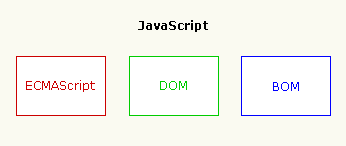
\includegraphics[scale=0.5]{js_arch.png}
\vspace{-20pt}
\caption{JavaScript模型}
\label{js_arch}
\end{figure}


在 ECMA-262 中,ECMAScript 符合性(conformance)有明确的定义。一个脚本语言必须满足以下四项基本原则:

\begin{compactitem}
\item 符合的实现必须按照 ECMA-262 中所描述的支持所有的“类型、值、对象、属性、函数和程序语言及语义”(ECMA-262,第一页)
\item 符合的实现必须支持 Unicode 字符标准(UCS)
\item 符合的实现可以增加没有在 ECMA-262 中指定的“额外类型、值、对象、属性和函数”。ECMA-262 将这些增加描述为规范中未给定的新对象或对象的新属性
\item 符合的实现可以支持没有在 ECMA-262 中定义的“程序和正则表达式语法”(意思是可以替换或者扩展内建的正则表达式支持)
\end{compactitem}

所有 ECMAScript 实现必须符合以上标准。

ECMAScript 仅仅是一个描述,定义了脚本语言的所有属性、方法和对象。其他语言可以实现 ECMAScript 来作为功能的基准,例如,JavaScript 就是这样:

\begin{figure}[!h]
\centering
\begin{tikzpicture}[sibling distance=80pt]
\tikzset{
box/.style={ rectangle , rounded corners=5pt ,
minimum width=50pt , minimum height=20pt , inner sep=5pt ,
draw=Silver ,fill=Lavender }
}

\node[box]{ECMAScript}
	child {node[box] {JavaScript}}
	child {node[box] {ActionScript}}
	child {node[box] {ScriptEase}};

\end{tikzpicture}
\caption{ECMAScript实现}
\label{ECMAScript_implement}
\end{figure}

每个浏览器都有它自己的 ECMAScript 接口的实现,然后这个实现又被扩展,包含了 DOM 和 BOM。当然还有其他实现并扩展了 ECMAScript 的语言,例如 Windows 脚本宿主(Windows Scripting Host, WSH)、Macromedia 在 Flash 和 Director MX 中的 ActionScript,以及 Nombas ScriptEase。

ECMAScript 并不与任何具体浏览器相绑定,实际上,它也没有提到用于任何用户输入输出的方法(这点与 C 这类语言不同,它需要依赖外部的库来完成这类任务)。

ECMA-262 标准(第 2 段)中对ECMAScript的描述如下:

\vspace{20pt}

\textcolor{Blue}{“ECMAScript 可以为不同种类的宿主环境提供核心的脚本编程能力,因此核心的脚本语言是与任何特定的宿主环境分开进行规定的... ...”}

\vspace{20pt}



Web 浏览器对于 ECMAScript 来说是一个宿主环境,但它并不是唯一的宿主环境。事实上,还有不计其数的其他各种环境(例如 Nombas 的 ScriptEase,以及 Macromedia 同时用在 Flash 和 Director MX 中的 ActionScript)可以容纳 ECMAScript 实现。那么 ECMAScript 在浏览器之外规定了些什么呢?

简单地说,ECMAScript 描述了以下内容:

\begin{compactitem}
\item 语法
\item 类型
\item 语句
\item 关键字
\item 保留字
\item 运算符
\item 对象
\end{compactitem}





\chapter{Syntax}

ECMAScript借用了一些语言的语法,比如Java、C 和 Perl。其中,Java 和 ECMAScript 有一些关键的语法特性相同,也有一些完全不同。

\begin{compactenum}
\item 区分大小写

与 Java 一样,变量、函数名、运算符以及其他一切东西都是区分大小写的。比如,变量 test 与变量 TEST 是不同的。

JavaScript 语句和 JavaScript 变量都对大小写敏感。


\item 弱类型

与 Java 和 C 不同,ECMAScript 中的变量无特定的类型,也就是说,JavaScript变量是弱类型的。

定义变量时只用 var 运算符,可以将它初始化为任意值,在运行时可以随时改变变量所存数据的类型(不过应该尽量避免这样做)。

\begin{lstlisting}[language=JavaScript]
var color = "red";
var num = 25;
var visible = true;
\end{lstlisting}


\item 分号

Java、C 和 Perl 都要求每行代码以分号(;)结束才符合语法。

ECMAScript 则允许开发者自行决定是否以分号结束一行代码。如果没有分号,ECMAScript 就把折行代码的结尾看做该语句的结尾(与 Visual Basic 和 VBScript 相似),前提是这样没有破坏代码的语义。

最好的代码编写习惯是总加入分号,因为没有分号,有些浏览器就不能正确运行,不过根据 ECMAScript 标准,下面两行代码都是正确的:

\begin{lstlisting}[language=JavaScript]
var test1 = "red"
var test2 = "blue";
\end{lstlisting}

\item 注释

ECMAScript 借用了Java、C 和 PHP 语言的注释语法。

在ECMAScript中可以使用两种类型的注释:

\begin{compactitem}
\item 单行注释以双斜杠开头(//)
\item 多行注释以单斜杠和星号开头(/*),以星号和单斜杠结尾(*/)
\end{compactitem}

\begin{lstlisting}[language=JavaScript]
//this is a single-line comment

/*this is a multi-
line comment*/
\end{lstlisting}


\item 代码块

ECMAScript从 Java 中借鉴的另一个概念是代码块。

代码块表示一系列应该按顺序执行的语句,这些语句被封装在左括号(\texttt{\{})和右括号(\texttt{\}})之间。

\begin{lstlisting}[language=JavaScript]
if (test1 == "red") {
    test1 = "blue";
    alert(test1);
}
\end{lstlisting}

\end{compactenum}







\chapter{Variable}

变量是存储信息的容器,ECMAScript规定使用 var 运算符声明变量,而且变量名需要遵守一些简单的规则。

\section{Variable Naming}




变量可以使用短名称(比如 x 和 y),也可以使用描述性更好的名称(比如 age, sum, totalvolume),而且JavaScript 语句和 JavaScript 变量都对大小写敏感。

\begin{compactitem}
\item 变量必须以字母开头
\item 变量也能以 \$ 和 \_ 符号开头(不推荐这么做)
\item 变量名称对大小写敏感(y 和 Y 是不同的变量)
\end{compactitem}

只是因为变量名的语法正确,并不意味着就该使用它们,因此变量还应遵守以下某条著名的命名规则:

\begin{compactitem}
\item Camel 标记法

首字母是小写的,接下来的字母都以大写字符开头。例如:

\begin{lstlisting}[language=JavaScript]
var myTestValue = 0, mySecondValue = "hi";
\end{lstlisting}

在面向对象的语言中,使用 camel-case 标记法的函数是很常见的。


\item Pascal 标记法

首字母是大写的,接下来的字母都以大写字符开头。例如:

\begin{lstlisting}[language=JavaScript]
var MyTestValue = 0, MySecondValue = "hi";
\end{lstlisting}

\item 匈牙利类型标记法

在以 Pascal 标记法命名的变量前附加一个小写字母(或小写字母序列),说明该变量的类型。例如,i 表示整数,s 表示字符串,如下所示:

\begin{lstlisting}[language=JavaScript]
var iMyTestValue = 0, sMySecondValue = "hi";
\end{lstlisting}

\end{compactitem}


\begin{longtable}{|m{120pt}|m{80pt}|m{80pt}|}
%head
\multicolumn{3}{r}{}
\tabularnewline\hline
类型	&前缀	&示例
\endhead
%endhead

%firsthead
\hline
类型	&前缀	&示例
\endfirsthead
%endfirsthead

%foot
\multicolumn{3}{r}{}
\endfoot
%endfoot

%lastfoot
\endlastfoot
%endlastfoot

\hline
数组					& a	&aValues\\
\hline
布尔型					& b	&bFound\\
\hline
浮点型(数字)			&f	&fValue\\
\hline
函数					&fn	&fnMethod\\
\hline
整型(数字)			&i	&iValue\\
\hline
对象					& o	&oType\\
\hline
正则表达式				& re&rePattern\\
\hline
字符串					& s	&sValue\\
\hline
变型(可以是任何类型)&v	&vValue\\
\hline
\end{longtable}




\section{Variable Declaration}

ECMAScript 中的变量是用 var 运算符(variable 的缩写)加变量名定义的。在 JavaScript 中创建变量时,通常称为“声明”变量。

在计算机程序中,经常会声明无值的变量。与 Java 不同的是,ECMAScript 中的变量并不一定要初始化(它们是在幕后初始化的)。因此,下面这一行代码也是有效的:




\begin{lstlisting}[language=JavaScript]
var x;
\end{lstlisting}

这样变量声明之后,该变量是空的(它没有值)。未使用值来声明的变量,其值实际上是 undefined。在执行过上述语句后,变量 x 的值将是 undefined。

此外,与 Java 不同的还有就是,ECMAScript变量可以存放不同类型的值,这是弱类型变量的优势,解释程序会为变量自动创建一个数据类型,无需明确的类型声明。例如,可以把变量初始化为字符串类型的值,之后把它设置为数字值,如下所示:

\begin{lstlisting}[language=JavaScript]
var test = "hi";
alert(test);
test = 55;
alert(test);
\end{lstlisting}

这段代码将毫无问题地输出字符串值和数字值。但是,如前所述,使用变量时,好的编码习惯是始终存放相同类型的值。


还可以在一条语句中声明很多变量,而且用同一个 var 语句定义的变量不必具有相同的类型,在 ECMAScript 中这样定义也是完全合法的。如下所示:

\begin{lstlisting}[language=JavaScript]
var name="Gates", age=56, job="CEO";

var name="Gates",
age=56,
job="CEO";
\end{lstlisting}

该语句以 var 开头,并使用逗号分隔变量即可,而且上述也表明变量声明可以横跨多行。

ECMAScript 另一个有趣的方面(也是与大多数程序设计语言的主要区别),是在使用变量之前不必声明。例如:


\begin{lstlisting}[language=JavaScript]
var sTest = "hello ";
sTest2 = sTest + "world";
alert(sTest2);
\end{lstlisting}


在上面的代码中,首先,sTest 被声明为字符串类型的值 "hello"。接下来的一行,用变量 sTest2 把 sTest 与字符串 "world" 连在一起。变量 sTest2 并没有用 var 运算符定义,这里只是插入了它,就像已经声明过它一样。

ECMAScript 的解释程序遇到未声明过的标识符时,用该变量名创建一个全局变量,并将其初始化为指定的值。

这是该语言的便利之处,不过如果不能紧密跟踪变量,这样做也很危险。最好的习惯是像使用其他程序设计语言一样,总是声明所有变量。

\section{Variable Asignment}


变量声明之后,此时该变量是空的(它没有值),如需向变量赋值,可以使用等号,不过也可以在声明变量时就对其赋值\footnote{一个好的编程习惯是,在代码开始处,统一对需要的变量进行声明。}:

\begin{lstlisting}[language=JavaScript]
var test = "hi";
var x=2;
var y=3;
var z=x+y;
\end{lstlisting}



在代数中,可以使用字母(比如 x)来保存值(比如 2)和表达式(比如 z=x+y)。

就像代数那样,可以通过 JavaScript 变量来做算数,使用的是 = 和 + 这类运算符:通过上面的表达式 z=x+y,就能够计算出 z 的值为 5。

在下面的例子中创建了名为 carname 的变量,并向其赋值 "Benz",然后把它放入 id="demo" 的 HTML 段落中:

\begin{lstlisting}[language=HTML]
<p id="demo"></p>
<script>
  var carname="Benz"
  document.getElementById("demo").innerHTML=carname;
</script>
\end{lstlisting}

如果重新声明 JavaScript 变量,该变量的值不会丢失,例如在以下两条语句执行后,变量 carname 的值依然是 "Benz":

\begin{lstlisting}[language=JavaScript]
var carname="Benz";
var carname;
\end{lstlisting}




JavaScript 变量还能保存其他数据类型,比如文本值 (name="Bill Gates")。当向变量分配文本值时,应该用双引号或单引号包围这个值。

当向变量赋的值是数值时,不要使用引号。如果用引号包围数值,该值会被作为文本来处理。


\begin{lstlisting}[language=JavaScript]
var pi=3.14;
var name="Bill Gates";
var answer='Yes I am!';
\end{lstlisting}





\chapter{Keywords}



ECMA-262 定义了 ECMAScript 支持的关键字(keyword),这些关键字标识了 ECMAScript 语句的开头和/或结尾。根据规定,关键字是保留的,不能用作变量名或函数名\footnote{注意:如果把关键字用作变量名或函数名,可能得到诸如 "Identifier Expected"(应该有标识符、期望标识符)这样的错误消息。}。

下面是 ECMAScript 关键字的完整列表:



\begin{table}[htbp]
\centering
\caption{ECMAScript Keywords}
\label{ecmascrpit_keywords}
\rowcolors{1}{White}{Lavender}
\begin{tabular}{m{65pt}m{65pt}m{65pt}m{65pt}m{65pt}}
break	&case	&catch	&continue	&default\\
delete	&do	&else	&finally		&for\\
function	&if		&in		&instanceof	&new\\
return	&switch&this	&throw		&try\\
typeof	&var	&void	&while		&with\\
\end{tabular}
\end{table}



\chapter{Reserved words}



ECMA-262 定义了 ECMAScript 支持的保留字(reserved word)。

保留字在某种意思上是为将来的关键字而保留的单词,因此保留字不能被用作变量名或函数名\footnote{注意:如果将保留字用作变量名或函数名,那么除非将来的浏览器实现了该保留字,否则很可能收不到任何错误消息。当浏览器将其实现后,该单词将被看做关键字,如此将出现关键字错误。}。

ECMA-262 第三版中保留字的完整列表如下:



\begin{table}[htbp]
\centering
\caption{ECMAScript Reserved Words}
\label{ecmascrpit_reserved_words}
\rowcolors{1}{White}{Lavender}
\begin{tabular}{m{65pt}m{65pt}m{65pt}m{65pt}m{65pt}}
abstract	&boolean	&byte	&char	&class\\
const		&debugger	&double&enum	&export\\
extends		&final		&float	&goto	&implements\\
import		&int		&interface&long	&native\\
package		&private	&protected	&public&short\\
static		&super		&synchronized&throws&transient\\
volatile		&			&			&	&\\
\end{tabular}
\end{table}



\chapter{Value}
\vspace{-20pt}
在 ECMAScript 中,变量可以存在两种类型的值,即原始值和引用值。

\begin{compactitem}
\item 原始值

存储在栈(stack)中的简单数据段,也就是说,它们的值直接存储在变量访问的位置。

\item 引用值

存储在堆(heap)中的对象,也就是说,存储在变量处的值是一个指针(point),指向存储对象的内存处。

\end{compactitem}

为变量赋值时,ECMAScript 的解释程序必须判断该值是原始类型,还是引用类型。要实现这一点,解释程序则需尝试判断该值是否为 ECMAScript 的原始类型之一,即 Undefined、Null、Boolean、Number 和 String 型。由于这些原始类型占据的空间是固定的,所以可将他们存储在较小的内存区域~——~栈中,这样存储便于迅速查寻变量的值。


\begin{figure}[!h]
\centering
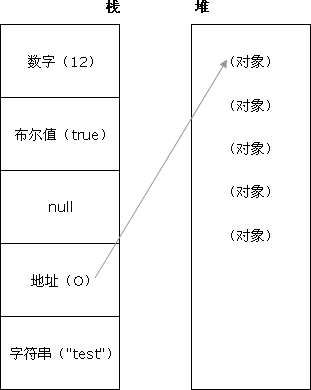
\includegraphics[scale=0.5]{js_value.png}
\vspace{-10pt}
\caption{Stack \& Heap}
\label{stack_heap}
\end{figure}

如果一个值是引用类型的,那么它的存储空间将从堆中分配。由于引用值的大小会改变,所以不能把它放在栈中,否则会降低变量查寻的速度。相反,放在变量的栈空间中的值是该对象存储在堆中的地址。地址的大小是固定的,所以把它存储在栈中对变量性能无任何负面影响。

在许多语言中,字符串都被看作引用类型,而非原始类型,因为字符串的长度是可变的,但是ECMAScript 打破了这一传统。

ECMAScript 有 5 种原始类型(primitive type),即 Undefined、Null、Boolean、Number 和 String。

ECMA-262 把术语类型(type)定义为值的一个集合,每种原始类型定义了它包含的值的范围及其字面量表示形式。




JavaScript 拥有动态类型,这意味着相同的变量可用作不同的类型:

\begin{lstlisting}[language=JavaScript]
var x                // x 为 undefined
var x = 6;           // x 为数字
var x = "Bill";      // x 为字符串
\end{lstlisting}

ECMAScript 有 5 种原始类型(primitive type),即 Undefined、Null、Boolean、Number 和 String。

声明新变量时,可以使用关键词 "new" 来声明其类型:

\begin{lstlisting}[language=JavaScript]
var carname=new String;
var x=      new Number;
var y=      new Boolean;
var cars=   new Array;
var person= new Object;
\end{lstlisting}

JavaScript 中的所有事物都是对象:字符串、数字、数组、日期等,因此JavaScript 变量均为对象,当声明一个变量时,就创建了一个新的对象。












\chapter{Primitive Types}




\section{Typeof Operator}


ECMAScript 提供了 typeof 运算符来判断一个值是否在某种类型的范围内,可以typeof运算符判断一个值是否表示一种原始类型:如果它是原始类型,还可以判断它表示哪种原始类型。

typeof 运算符有一个参数,即要检查的变量或值。例如:



\begin{lstlisting}[language=JavaScript]
var sTemp = "test string";
alert (typeof sTemp);    //输出 "string"
alert (typeof 86);    //输出 "number"
\end{lstlisting}



对变量或值调用 typeof 运算符将返回下列值之一:

\begin{compactitem}
\item undefined - 如果变量是 Undefined 类型的
\item boolean - 如果变量是 Boolean 类型的
\item number - 如果变量是 Number 类型的
\item string - 如果变量是 String 类型的
\item object - 如果变量是一种引用类型或 Null\footnote{至于为什么 typeof 运算符对于 null 值会返回 "Object"。这实际上是 JavaScript 最初实现中的一个错误,然后被 ECMAScript 沿用了。现在,null 被认为是对象的占位符,从而解释了这一矛盾,但从技术上来说,它仍然是原始值。}类型的
\end{compactitem}





\section{Undefined}


Undefined 类型只有一个值,即 undefined。当声明的变量未初始化时,该变量的默认值是 undefined。



\begin{lstlisting}[language=JavaScript]
var oTemp;
var sTemp = "test string";
alert (typeof sTemp);    	//输出 "string"
alert(typeof oTemp);	//输出"undefined"
alert (typeof 86);    		//输出 "number"
alert(oTemp == undefined);
\end{lstlisting}

虽然,值 undefined 并不同于未定义的值。但是,typeof 运算符并不真正区分这两种值。考虑下面的代码:


\begin{lstlisting}[language=JavaScript]
var oTemp;

alert(typeof oTemp);  //输出 "undefined"
alert(typeof oTemp2);  //输出 "undefined"
\end{lstlisting}


前面的代码对两个变量输出的都是 "undefined",即使只有变量 oTemp2 从未被声明过。如果对 oTemp2 使用除 typeof 之外的其他运算符的话,会引起错误,因为其他运算符只能用于已声明的变量上。例如,下面的代码将引发错误:

\begin{lstlisting}[language=JavaScript]
var oTemp;
alert(oTemp2 == undefined);
\end{lstlisting}

另外,当函数无明确返回值时,返回的也是值 "undefined",如下所示:



\begin{lstlisting}[language=JavaScript]
function testFunc() {
}

alert(testFunc() == undefined);  //输出 "true"
\end{lstlisting}


\section{Null}


另一种只有一个值的类型是 Null,它只有一个专用值 null,即它的字面量。值 undefined 实际上是从值 null 派生来的,因此 ECMAScript 把它们定义为相等的,Undefined 这个值表示变量不含有值,可以通过将变量的值设置为 null 来清空变量。



\begin{lstlisting}[language=JavaScript]
cars=null;
person=null;
alert(typeof cars);	//输出“object”
alert(typeof persion);	//输出“object”
alert(null == undefined);  //输出 "true"
\end{lstlisting}

尽管这两个值相等,但它们的含义不同。undefined 是声明了变量但未对其初始化时赋予该变量的值,null 则用于表示尚未存在的对象。如果函数或方法要返回的是对象,那么找不到该对象时,返回的通常是 null。





\section{Boolean}


Boolean 类型是 ECMAScript 中最常用的类型之一,它有两个值 true 和 false (即两个 Boolean 字面量),常用在条件测试中。。


即使 false 不等于 0,0 也可以在必要时被转换成 false,这样在 Boolean 语句中使用两者都是安全的。


\begin{lstlisting}[language=JavaScript]
var bFound = true;
var bLost = false;
\end{lstlisting}





\section{Number}

ECMA-262 中定义的最特殊的类型是 Number 类型,JavaScript 只有一种数字类型,数字可以带小数点,也可以不带。

\begin{lstlisting}[language=JavaScript]
var x1=34.00;      //使用小数点来写
var x2=34;         //不使用小数点来写
\end{lstlisting}



Number类型既可以表示 32 位的整数,还可以表示 64 位的浮点数。直接输入的(而不是从另一个变量访问的)任何数字都被看做 Number 类型的字面量。例如,下面的代码声明了存放整数值的变量,它的值由字面量 86 定义:


\begin{lstlisting}[language=JavaScript]
var iNum = 86;
alert(iNum == number);
alert (typeof 86);    		//输出 "number"
\end{lstlisting}


\subsection{Octal Number}


整数也可以被表示为八进制(以 8 为底)或十六进制(以 16 为底)的字面量\footnote{尽管所有整数都可以表示为八进制或十六进制的字面量,但所有数学运算返回的都是十进制结果。}。八进制字面量的首数字必须是 0,其后的数字可以是任何八进制数字(0-7),如下面的代码所示:



\begin{lstlisting}[language=JavaScript]
var iNum = 86;		//十进制数86
var iNum = 070;  	//070 等于十进制的 56
\end{lstlisting}


\subsection{Hex Number}



要创建十六进制的字面量,首位数字必须为 0,后面接字母 x,然后是任意的十六进制数字(0 到 9 和 A 到 F)。这些字母可以是大写的,也可以是小写的。例如:



\begin{lstlisting}[language=JavaScript]
var iNum = 0x1f;  //0x1f 等于十进制的 31
var iNum = 0xAB;  //0xAB 等于十进制的 171
\end{lstlisting}


\subsection{Float Number}


要定义浮点值,必须包括小数点和小数点后的一位数字(例如,用 1.0 而不是 1)。这被看作浮点数字面量。例如:


\begin{lstlisting}[language=JavaScript]
var iNum = 86;		//十进制数86
var iNum = 070;  	//070 等于十进制的 56
var iNum = 0x1f;  	//0x1f 等于十进制的 31
var iNum = 0xAB;  	//0xAB 等于十进制的 171
var fNum = 5.0;		//浮点数5.0
\end{lstlisting}

对于浮点字面量的有趣之处在于,用它进行计算前,真正存储的是字符串。


\subsection{Infinity}


对于非常大或非常小的数,可以用科学计数法表示浮点数,从而可以把一个数表示为数字(包括十进制数字)加 e(或 E),后面加乘以 10 的倍数。例如:


\begin{lstlisting}[language=JavaScript]
var iNum = 86;			//十进制数86
var iNum = 070;  		//070 等于十进制的 56
var iNum = 0x1f;  		//0x1f 等于十进制的 31
var iNum = 0xAB;  		//0xAB 等于十进制的 171
var fNum = 5.0;			//浮点数5.0
var fNum = 5.618e7;	//浮点数 56180000
var y=123e5;      // 12300000
var z=123e-5;     // 0.00123
\end{lstlisting}

该符号表示的是数 56180000。把科学计数法转化成计算式就可以得到该值:$\text{5.618}\times \text{10}^{\text{7}}$。


\subsection{Scientific notation}




也可以用科学计数法表示非常小的数,例如 0.00000000000000008 可以表示为$\text{8}\times e^{-\text{17}}$(这里,10 被升到 -17 次幂,意味着需要被 10 除 17 次)。ECMAScript 默认把具有 6 个或 6 个以上前导 0 的浮点数转换成科学计数法。

也可用 64 位 IEEE 754 形式存储浮点值,这意味着十进制值最多可以有 17 个十进制位。17 位之后的值将被裁去,从而造成一些小的数学误差。


几个特殊值也被定义为 Number 类型,其中前两个是 Number.MAX\_VALUE 和 Number.MIN\_VALUE,它们定义了 Number 值集合的外边界。所有 ECMAScript 数都必须在这两个值之间,不过计算生成的数值结果可以不落在这两个值之间。

当计算生成的数大于 Number.MAX\_VALUE 时,它将被赋予值 Number.POSITIVE\_INFINITY,意味着不再有数字值。同样,生成的数值小于 Number.MIN\_VALUE 的计算也会被赋予值 Number.NEGATIVE\_INFINITY,也意味着不再有数字值。如果计算返回的是无穷大值,那么生成的结果不能再用于其他计算。

事实上,有专门的值表示无穷大,(如你猜到的)即 Infinity。Number.POSITIVE\_INFINITY 的值为 Infinity。Number.NEGATIVE\_INFINITY 的值为 -Infinity。

由于无穷大数可以是正数也可以是负数,所以可用一个方法判断一个数是否是有穷的(而不是单独测试每个无穷数)。可以对任何数调用 isFinite() 方法,以确保该数不是无穷大。例如:



\begin{lstlisting}[language=JavaScript]
var iResult = iNum * some_really_large_number;

if (isFinite(iResult)) {
    alert("finite");
}

else {
    alert("infinite");
}
\end{lstlisting}


\subsection{NaN}


最后一个特殊值是 NaN,表示非数(Not a Number)。NaN 是个奇怪的特殊值。一般说来,这种情况发生在类型(String、Boolean 等)转换失败时。例如,要把单词 blue 转换成数值就会失败,因为没有与之等价的数值。与无穷大一样,NaN 也不能用于算术计算。NaN 的另一个奇特之处在于,它与自身不相等,这意味着下面的代码将返回 false:


\begin{lstlisting}[language=JavaScript]
alert(NaN == NaN);  //输出 "false"
\end{lstlisting}

出于这个原因,不推荐使用 NaN 值本身。函数 isNaN() 会做得相当好:

\begin{lstlisting}[language=JavaScript]
alert(isNaN("blue"));  //输出 "true"
alert(isNaN("666"));  //输出 "false"
\end{lstlisting}

JavaScript最早是在HTML网页上使用,用来给HTML网页增加动态功能,比如JavaScript 常用于验证用户的输入,比如在下面的例子中,如果输入值不是数字,浏览器会弹出提示框。



\begin{lstlisting}[language=HTML]
<input id="demo" type="text">

<script>
function myFunction()
{
var x=document.getElementById("demo").value;
if(x==""||isNaN(x))
	{
	alert("Not Numeric");
	}
}
</script>

<button type="button" onclick="myFunction()">点击这里</button>
\end{lstlisting}



\section{String}

JavaScript 变量还能保存其他数据类型,比如文本值 (name="Bill Gates"),这又称为String类型。

String 类型的独特之处在于,它是唯一没有固定大小的原始类型,可以用字符串存储 0 或更多的 Unicode 字符,由16 位整数表示。

字符串中每个字符都有特定的位置,首字符从位置 0 开始,第二个字符在位置 1,依此类推。这意味着字符串中的最后一个字符的位置一定是字符串的长度减 1:

\begin{figure}[!h]
\centering
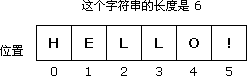
\includegraphics[scale=0.5]{js_string.png}
\caption{EMAScript String 类型}
\label{js_string}
\end{figure}

JavaScript字符串字面量是由双引号(")或单引号(')声明的,字符串可以是引号中的任意文本,因此当向变量赋的值是数值时,不要使用引号。如果用引号包围数值,该值会被作为文本来处理。

由于 ECMAScript 没有字符类型,所以JavaScript可使用这两种表示法中的任何一种。Java 则是用双引号声明字符串,用单引号声明字符。例如,下面的两行JavaScript代码都有效:


\begin{lstlisting}[language=JavaScript]
var sColor1 = "red";
var sColor2 = 'red';
\end{lstlisting}



可以在字符串中使用引号,只要不匹配包围字符串的引号即可:


\begin{lstlisting}[language=JavaScript]
var answer="Nice to meet you!";
var answer="He is called 'Bill'";
var answer='He is called "Bill"';
\end{lstlisting}




String 类型还包括几种字符字面量,Java、C 和 Perl 的开发者应该对此非常熟悉,在下面的表格中列出了 ECMAScript 的字符字面量:

\begin{longtable}{|m{50pt}|m{300pt}|}
%head
\multicolumn{2}{r}{}
\tabularnewline\hline
字面量	&含义
\endhead
%endhead

%firsthead
\caption{ECMAScript 的字符字面量}\\
\hline
字面量	&含义
\endfirsthead
%endfirsthead

%foot
\multicolumn{2}{r}{}
\endfoot
%endfoot

%lastfoot
\endlastfoot
%endlastfoot

\hline
\verb|\n|	&换行\\
\hline
\verb|\t|	&制表符\\
\hline
\verb|\b|	&空格\\
\hline
\verb|\r|	&回车\\
\hline
\verb|\f|	&换页符\\
\hline
\verb|\\|	&反斜杠\\
\hline
\verb|\'|	&单引号\\
\hline
\verb|\"|	&双引号\\
\hline
\verb|\0nnn|	&八进制代码 nnn 表示的字符(n 是 0 到 7 中的一个八进制数字)\\
\hline
\verb|\xnn|	&十六进制代码 nn 表示的字符(n 是 0 到 F 中的一个十六进制数字)\\
\hline
\verb|\unnnn|	&十六进制代码 nnnn 表示的 Unicode 字符(n 是 0 到 F 中的一个十六进制数字)\\
\hline

\end{longtable}



\section{Array}

下面的代码创建名为 cars 的数组:

\begin{lstlisting}[language=JavaScript]
var cars=new Array();
cars[0]="Audi";
cars[1]="BMW";
cars[2]="Volvo";
\end{lstlisting}

或者 (condensed array):


\begin{lstlisting}[language=JavaScript]
var cars=new Array("Audi","BMW","Volvo");
\end{lstlisting}

或者 (literal array):

\begin{lstlisting}[language=JavaScript]
var cars=["Audi","BMW","Volvo"];
\end{lstlisting}

数组下标是基于零的,所以第一个项目是 [0],第二个是 [1],以此类推。


\chapter{Type Conversion}

所有程序设计语言最重要的特征之一是具有进行类型转换的能力,ECMAScript 给开发者提供了大量简单的类型转换方法。

大部分类型具有进行简单转换的方法,还有几个全局方法可以用于更复杂的转换。无论哪种情况,在 ECMAScript 中,类型转换都是简短的一步操作。


\section{String}

ECMAScript 的 Boolean 值、数字和字符串的原始值的有趣之处在于它们是伪对象,这意味着它们实际上具有属性和方法。例如,要获得字符串的长度,可以采用下面的代码:

\begin{lstlisting}[language=JavaScript]
var sColor = "red";
alert(sColor.length);	//输出 "3"
\end{lstlisting}


尽管 "red" 是原始类型的字符串,它仍然具有属性 length,用于存放字符串的大小。总而言之,3 种主要的原始类型 Boolean 值、数字和字符串都有 toString() 方法,可以把它们的值转换成字符串。

ECMAScript 定义所有对象都有 toString() 方法,无论它是伪对象,还是真对象。因为 String 类型属于伪对象,所以它一定有 toString() 方法。


\subsection{Boolean}


Boolean 类型的 toString() 方法只是输出 "true" 或 "false",结果由变量的值决定:


\begin{lstlisting}[language=JavaScript]
var bFound = false;
alert(bFound.toString());	//输出 "false"
\end{lstlisting}




\subsection{Number}

Number 类型的 toString() 方法比较特殊,它有两种模式,即默认模式和基模式。采用默认模式,toString() 方法只是用相应的字符串输出数字值(无论是整数、浮点数还是科学计数法),如下所示:


\begin{lstlisting}[language=JavaScript]
var iNum1 = 10;
var iNum2 = 10.0;
alert(iNum1.toString());	//输出 "10"
alert(iNum2.toString());	//输出 "10"
\end{lstlisting}



在默认模式中,无论最初采用什么表示法声明数字,Number 类型的 toString() 方法返回的都是数字的十进制表示。因此,以八进制或十六进制字面量形式声明的数字输出的都是十进制形式的。


采用 Number 类型的 toString() 方法的基模式,可以用不同的基输出数字,基只是要转换成的基数的另一种加法而已,它是 toString() 方法的参数,例如二进制的基是 2,八进制的基是 8,十六进制的基是 16。



\begin{lstlisting}[language=JavaScript]
var iNum = 10;
alert(iNum.toString(2));	//输出 "1010"
alert(iNum.toString(8));	//输出 "12"
alert(iNum.toString(16));	//输出 "A"
\end{lstlisting}


在上面的示例中,以 3 种不同的形式输出了数字 10,即二进制形式、八进制形式和十六进制形式\footnote{对数字调用 toString(10) 与调用 toString() 相同,它们返回的都是该数字的十进制形式。}。

HTML 采用十六进制表示每种颜色,在 HTML 中处理数字时这种功能非常有用。


\begin{compactitem}
\item arrayObject.toString()
\item booleanObject.toString()
\item dateObject.toString()
\item NumberObject.toString()
\item stringObject.toString()
\end{compactitem}



\section{Number}


ECMAScript 提供了两种把非数字的原始值转换成数字的方法,即 parseInt() 和 parseFloat(),其中前者把值转换成整数,后者把值转换成浮点数。只有对 String 类型调用这些方法,它们才能正确运行,对其他类型返回的都是 NaN。


\subsection{parseInt()}

在判断字符串是否是数字值前,parseInt() 和 parseFloat() 都会仔细分析该字符串。

parseInt() 方法首先查看位置 0 处的字符,判断它是否是个有效数字;如果不是,该方法将返回 NaN,不再继续执行其他操作。但如果该字符是有效数字,该方法将查看位置 1 处的字符,进行同样的测试。这一过程将持续到发现非有效数字的字符为止,此时 parseInt() 将把该字符之前的字符串转换成数字。例如,如果要把字符串 "12345red" 转换成整数,那么 parseInt() 将返回 12345,因为当它检查到字符 r 时,就会停止检测过程。

字符串中包含的数字字面量会被正确转换为数字,比如 "0xA" 会被正确转换为数字 10。不过,字符串 "22.5" 将被转换成 22,因为对于整数来说,小数点是无效字符。



\begin{lstlisting}[language=JavaScript]
var iNum1 = parseInt("12345red");	//返回 12345
var iNum1 = parseInt("0xA");	//返回 10
var iNum1 = parseInt("56.9");	//返回 56
var iNum1 = parseInt("red");	//返回 NaN
\end{lstlisting}

parseInt() 方法还有基模式,可以把二进制、八进制、十六进制或其他任何进制的字符串转换成整数(默认模式是十进制)。基是由 parseInt() 方法的第二个参数指定的,所以如果要解析十六进制的值,需如下调用 parseInt() 方法:


\begin{lstlisting}[language=JavaScript]
var iNum1 = parseInt("10", 2);	//返回 2
var iNum2 = parseInt("10", 8);	//返回 8
var iNum3 = parseInt("10", 10);	//返回 10
var iNum1 = parseInt("AF", 16);	//返回 175
\end{lstlisting}

如果十进制数包含前导 0,那么最好采用基数 10,这样才不会意外地得到八进制的值。例如:


\begin{lstlisting}[language=JavaScript]
var iNum1 = parseInt("010");	//返回 8
var iNum2 = parseInt("010", 8);	//返回 8
var iNum3 = parseInt("010", 10);	//返回 10
\end{lstlisting}

在这段代码中,两行代码都把字符 "010" 解析成一个数字。第一行代码把这个字符串看作八进制的值,解析它的方式与第二行代码(声明基数为 8)相同。最后一行代码声明基数为 10,所以 iNum3 最后等于 10。




\subsection{parseFloat()}

parseFloat() 方法与 parseInt() 方法的处理方式相似,从位置 0 开始查看每个字符,直到找到第一个非有效的字符为止,然后把该字符之前的字符串转换成整数。

不过,对于这个方法来说,第一个出现的小数点是有效字符。如果有两个小数点,第二个小数点将被看作无效的。parseFloat() 会把这个小数点之前的字符转换成数字。这意味着字符串 "11.22.33" 将被解析成 11.22。

使用 parseFloat() 方法的另一不同之处在于,字符串必须以十进制形式表示浮点数,而不是用八进制或十六进制。该方法会忽略前导 0,所以八进制数 0102 将被解析为 102。对于十六进制数 0xA,该方法将返回 NaN,因为在浮点数中,x 不是有效字符\footnote{注释:经测试,具体的浏览器实现会返回 0,而不是 NaN。}。

此外,parseFloat() 方法也没有基模式。



\begin{lstlisting}[language=JavaScript]
var fNum1 = parseFloat("12345red");	//返回 12345
var fNum2 = parseFloat("0xA");	//返回 NaN
var fNum3 = parseFloat("11.2");	//返回 11.2
var fNum4 = parseFloat("11.22.33");	//返回 11.22
var fNum5 = parseFloat("0102");	//返回 102
var fNum1 = parseFloat("red");	//返回 NaN
\end{lstlisting}



\section{Type Casting}


可以使用强制类型转换(type casting)\footnote{cast 有“铸造”之意,很贴合“强制转换”的意思。}来处理转换值的类型。使用强制类型转换可以访问特定的值,即使它是另一种类型的。

ECMAScript 中可用的 3 种强制类型转换如下:

\begin{compactitem}
\item Boolean(value) - 把给定的值转换成 Boolean 型;
\item Number(value) - 把给定的值转换成数字(可以是整数或浮点数);
\item String(value) - 把给定的值转换成字符串;
\end{compactitem}

用这三个函数之一转换值,将创建一个新值,存放由原始值直接转换成的值,但这会造成意想不到的后果。


\subsection{Boolean()}



当要转换的值是至少有一个字符的字符串、非 0 数字或对象时,Boolean() 函数将返回 true。如果该值是空字符串、数字 0、undefined 或 null,它将返回 false。可以用下面的代码测试 Boolean 型的强制类型转换:


\begin{lstlisting}[language=JavaScript]
var b1 = Boolean("");		//false - 空字符串
var b2 = Boolean("hello");		//true - 非空字符串
var b1 = Boolean(50);		//true - 非零数字
var b1 = Boolean(null);		//false - null
var b1 = Boolean(0);		//false - 零
var b1 = Boolean(new object());	//true - 对象
\end{lstlisting}



\subsection{Number()}

Number() 函数的强制类型转换与 parseInt() 和 parseFloat() 方法的处理方式相似,只是它转换的是整个值,而不是部分值。


parseInt() 和 parseFloat() 方法只转换第一个无效字符之前的字符串,因此 "1.2.3" 将分别被转换为 "1" 和 "1.2"。用 Number() 进行强制类型转换时,"1.2.3" 将返回 NaN,因为整个字符串值不能转换成数字。如果字符串值能被完整地转换,Number() 将判断是调用 parseInt() 方法还是 parseFloat() 方法。

下表说明了对不同的值调用 Number() 方法会发生的情况:

\begin{longtable}{|m{150pt}|m{100pt}|}
%head
\multicolumn{2}{r}{}
\tabularnewline\hline
用法	&结果
\endhead
%endhead

%firsthead
\hline
用法	&结果
\endfirsthead
%endfirsthead

%foot
\multicolumn{2}{r}{}
\endfoot
%endfoot

%lastfoot
\endlastfoot
%endlastfoot

\hline
Number(false)	&0\\
\hline
Number(true)	&1\\
\hline
Number(undefined)	&NaN\\
\hline
Number(null)	&0\\
\hline
Number("1.2")	&1.2\\
\hline
Number("12")	&12\\
\hline
Number("1.2.3")	&NaN\\
\hline
Number(new object())	&NaN\\
\hline
Number(50)	&50\\
\hline

\end{longtable}





\subsection{String()}

强制类型转换方法 String() 是最简单的,因为它可把任何值转换成字符串。


要执行这种强制类型转换,只需要调用作为参数传递进来的值的 toString() 方法,即把 12 转换成 "12",把 true 转换成 "true",把 false 转换成 "false",以此类推。

强制转换成字符串和调用 toString() 方法的唯一不同之处在于,对 null 和 undefined 值强制类型转换可以生成字符串而不引发错误:


\begin{lstlisting}[language=JavaScript]
var s1 = String(null);	//"null"
var oNull = null;
var s2 = oNull.toString();	//会引发错误
\end{lstlisting}

在处理 ECMAScript 这样的弱类型语言时,强制类型转换非常有用,不过应该确保使用值的正确。




\chapter{Reference Types}

引用类型通常叫做类(class)\footnote{注意:从传统意义上来说,ECMAScript 并不真正具有类。事实上,除了说明不存在类,在 ECMA-262 中根本没有出现“类”这个词。ECMAScript 定义了“对象定义”,逻辑上等价于其他程序设计语言中的类。},也就是说,遇到引用值,所处理的就是对象。

JavaScript 是面向对象的语言,但 JavaScript 不使用类,实际上JavaScript 基于 prototype,而不是基于类的。

JavaScript的对象是拥有属性和方法的特殊数据类型。其中,属性是与对象相关的值,而方法是能够在对象上执行的动作。

可以通过如下的语法访问对象的属性,调用对象的方法,而且上面列出的每种属性和方法都会被其他对象覆盖。

\begin{lstlisting}[language=JavaScript]
objectName.propertyName
objectName.methodName()
\end{lstlisting}

如果要访问字符串对象“Hello world!”的length属性,并且把将其转换为大写,可以通过如下的代码:


\begin{lstlisting}[language=JavaScript]
var message="Hello World!";
var x=message.length;
var y=message.toUpperCase();
alert(x);
alert(y);
\end{lstlisting}

JavaScript 中的所有事物都是对象:字符串、数字、数组、日期等,而且JavaScript 提供多个内建对象,比如 String、Date、Array 等。

此外,JavaScript 允许自定义对象,创建新对象有两种不同的方法:

\begin{compactitem}
\item 定义并创建对象的实例
\item 使用函数来定义对象,然后创建新的对象实例
\end{compactitem}





举例来说,汽车就是现实生活中的对象,其中汽车的属性有:



\begin{lstlisting}[language=JavaScript]
var car = new Object();
car.name=Fiat
car.model=500
car.weight=850kg
car.color=white 
\end{lstlisting}

也可以使用替代语法(使用对象 literals),即:

\begin{lstlisting}[language=JavaScript]
car = {name:"Fiat", model:"500", weight:"850kg",color:"white"};
\end{lstlisting}

\section{Object Constructor}

使用函数(对象构造器)来构造对象的语法如下:



\begin{lstlisting}[language=JavaScript]
function car(name, model, weight, color){
  this.name = name;
  this.model = model;
  this.weight = weight;
  this.color = color;
}
\end{lstlisting}

通过对象构造器,就可以创建新的对象实例,代码如下:

\begin{lstlisting}[language=JavaScript]
var car1 = new car("Fiat", model:"500", weight:"850kg",color:"white");
\end{lstlisting}

可以通过为对象赋值,向已有对象添加新属性,,代码如下:


\begin{lstlisting}[language=JavaScript]
car.name = "Fiat";
car.model = "500";
car.weight = "850kg";
car.color = "white";
\end{lstlisting}




汽车的属性包括名称、型号、重量、颜色等,而且所有汽车都有这些属性,但是每款车的属性都不尽相同。

方法只不过是附加在对象上的函数,下面是在构造器函数内部定义对象的方法:

\begin{lstlisting}[language=JavaScript]
function car(name, model, weight, color){
  this.name = name;
  this.model = model;
  this.weight = weight;
  this.color = color;

  this.start = start;
  function start(){
  
  }
  ...
}
\end{lstlisting}



汽车的方法有:


\begin{lstlisting}[language=JavaScript]
var car = new Object();
car.start()
car.drive()
car.brake()
\end{lstlisting}

汽车的方法可以是启动、驾驶、刹车等。所有汽车都拥有这些方法,但是它们被执行的时间都不尽相同。

另一个对象构造的例子如下:

\begin{lstlisting}[language=JavaScript]
function person(firstname,lastname,age,eyecolor){
  this.firstname=firstname;
  this.lastname=lastname;
  this.age=age;
  this.eyecolor=eyecolor;

  this.changeName=changeName;
  function changeName(name){
    this.lastname=name;
  }
}
\end{lstlisting}


其中,changeName() 函数 name 的值赋给 person 的 lastname 属性,下面是使用函数对对象执行操作的示例:


\begin{lstlisting}[language=JavaScript]
var myFather=new person("Jim","Green",30,"blue");
var myMother=new person("Meimei","Han",28,"black");
myMother.changeName("Jane");
\end{lstlisting}

JavaScript for...in 语句循环可以遍历对象的属性,for...in 循环中的代码块将针对每个属性执行一次,语法如下:

\begin{lstlisting}[language=JavaScript]
for (对象中的变量){
  要执行的代码
}
\end{lstlisting}

下面的示例将循环遍历对象的属性:

\begin{lstlisting}[language=JavaScript]
var person={fname:"Jim",lname:"Green",age:30};

for (x in person){
  txt=txt + person[x];
}
\end{lstlisting}




\section{Object}

在 JavaScript 中,对象是数据(变量),拥有属性和方法,当声明一个 JavaScript 变量时,实际上就已经创建了一个对象,比如:

\begin{lstlisting}[language=JavaScript]
var u;
var bFound = true;
var iNum = 2013;
var cars=new Array("Audi","BMW","Volvo");
var sTxt = "Hello";
\end{lstlisting}

字符串对象拥有内建的属性 length,因此对于上面的字符串来说,length 的值是 5,同时字符串对象同时拥有若干个内建的方法。

在面向对象的语言中,属性和方法常被称为对象的成员,以上例中的sTxt字符串变量为例,就是:

\begin{lstlisting}[language=JavaScript]
txt.length=5
txt.indexOf()
txt.replace()
txt.search()
\end{lstlisting}


JavaScript 中的几乎所有事物都是对象:字符串、数字、数组、日期、函数等,可以由 new 运算符加上要实例化的对象的名字创建。例如,下面的代码创建 Object 对象的实例:


\begin{lstlisting}[language=JavaScript]
var o = new Object();
\end{lstlisting}

创建新 JavaScript 对象有很多不同的方法,并且还可以向已存在的对象添加属性和方法。下面创建名为 "person" 的对象,并为其添加了四个属性:

\begin{lstlisting}[language=JavaScript]
var person = new Object();
person.firstname="Jim";
person.lastname="Green";
person.age=30;
person.eyecolor="green";
\end{lstlisting}



这种语法与 Java 语言的相似,不过当有不止一个参数时,ECMAScript 要求使用括号。如果没有参数,如以下代码所示,括号可以省略\footnote{注意:尽管括号不是必需的,但是为了避免混乱,最好使用括号。}:

\begin{lstlisting}[language=JavaScript]
var o = new Object;
\end{lstlisting}

Object 对象自身用处不大,只是ECMAScript 中的 Object 对象与 Java 中的 java.lang.Object 相似,ECMAScript 中的所有对象都由这个对象继承而来,Object 对象中的所有属性和方法都会出现在其他对象中,所以理解了 Object 对象,就可以更好地理解其他对象。

Object 对象具有下列属性:

\begin{compactitem}
\item constructor
对创建对象的函数的引用(指针)。对于 Object 对象,该指针指向原始的 Object() 函数。
\item Prototype
对该对象的对象原型的引用。对于所有的对象,它默认返回 Object 对象的一个实例。
\end{compactitem}




Object 对象具有下列方法:

\begin{compactitem}
\item hasOwnProperty(property)
判断对象是否有某个特定的属性。必须用字符串指定该属性。(例如,o.hasOwnProperty("name"))
\item IsPrototypeOf(object)
判断该对象是否为另一个对象的原型。
\item PropertyIsEnumerable
判断给定的属性是否可以用 for...in 语句进行枚举。
\item ToString()
返回对象的原始字符串表示。对于 Object 对象,ECMA-262 没有定义这个值,所以不同的 ECMAScript 实现具有不同的值。
\item ValueOf()
返回最适合该对象的原始值。对于许多对象,该方法返回的值都与 ToString() 的返回值相同。
\end{compactitem}



对象由花括号分隔。在括号内部,对象的属性以名称和值对的形式 (name : value) 来定义,属性由逗号分隔:


\begin{lstlisting}[language=JavaScript]
var person={firstname:"Jim", lastname:"Green", id:1002};
\end{lstlisting}

上面例子中的对象 (person) 有三个属性:firstname、lastname 以及 id,空格和折行无关紧要。

JavaScript对象声明可横跨多行:


\begin{lstlisting}[language=JavaScript]
var person={
firstname : "Jim",
lastname  : "Green",
id        :  1002
};
\end{lstlisting}

对象属性有两种寻址方式:

\begin{lstlisting}[language=JavaScript]
name=person.lastname;
name=person["lastname"];
\end{lstlisting}


\section{Boolean Object}

Boolean 对象是 Boolean 原始类型的引用类型,用于将非逻辑值转换为逻辑值(true 或者 false)。


可以将 Boolean 对象理解为一个产生逻辑值的对象包装器,如果要创建 Boolean 对象,只需要传递 Boolean 值作为参数:



\begin{lstlisting}[language=JavaScript]
var oBooleanObject = new Boolean(true);
\end{lstlisting}



Boolean 对象将覆盖 Object 对象的 ValueOf() 方法,返回原始值,即 true 和 false。ToString() 方法也会被覆盖,返回字符串 "true" 或 "false"。但是,在 ECMAScript 中很少使用 Boolean 对象,即使使用,也不易理解。问题通常出现在 Boolean 表达式中使用 Boolean 对象时,例如:



\begin{lstlisting}[language=JavaScript]
var oFalseObject = new Boolean(false);
var bResult = oFalseObject && true;	//输出 true
\end{lstlisting}



在这段代码中,用 false 值创建 Boolean 对象,然后用这个值与原始值 true 进行 AND 操作。

在 Boolean 运算中,false 和 true 进行 AND 操作的结果是 false。不过,在上述这行代码中,计算的是 oFalseObject,而不是它的值 false\footnote{注意:虽然你应该了解 Boolean 对象的可用性,不过最好还是使用 Boolean 原始值,避免发生这一节提到的问题。}。

在 Boolean 表达式中,所有对象都会被自动转换为 true,所以 oFalseObject 的值是 true。然后 true 再与 true 进行 AND 操作,结果为 true。

如果逻辑对象无初始值或者其值为 0、-0、null、""、false、undefined 或者 NaN,那么对象的值为 false。否则,其值为 true(即使当自变量为字符串 "false" 时)。

下面的所有的代码行均会创建初始值为 false 的 Boolean 对象。


\begin{lstlisting}[language=JavaScript]
var myBoolean=new Boolean();
var myBoolean=new Boolean(0);
var myBoolean=new Boolean(null);
var myBoolean=new Boolean("");
var myBoolean=new Boolean(false);
var myBoolean=new Boolean(NaN);
\end{lstlisting}

下面的所有的代码行均会创初始值为 true 的 Boolean 对象:


\begin{lstlisting}[language=JavaScript]
var myBoolean=new Boolean(1);
var myBoolean=new Boolean(true);
var myBoolean=new Boolean("true");
var myBoolean=new Boolean("false");
var myBoolean=new Boolean("Jim Green");
\end{lstlisting}

\section{Number Object}


Number 对象是 Number 原始类型的引用类型。JavaScript 只有一种数字类型,可以使用也可以不使用小数点来书写数字,极大或极小的数字可通过科学(指数)计数法来写。

要创建 Number 对象,采用下列代码:

\begin{lstlisting}[language=JavaScript]
var oNumberObject = new Number(value);
var oNumberObject = Number(value);
\end{lstlisting}


JavaScript 不是类型语言。与许多其他编程语言不同,JavaScript 不定义不同类型的数字,比如整数、短、长、浮点等,JavaScript 中的所有数字都存储为根为 10 的 64 位(8 比特)的浮点数。

整数(不使用小数点或指数计数法)最多为 15 位,小数的最大位数是 17,但是浮点运算并不总是 100\% 准确。同样,如果前缀为 0,则 JavaScript 会把数值常量解释为八进制数,如果前缀为 0 和 "x",则解释为十六进制数。

Number对象的属性包括:

\begin{compactitem}
\item MAX\_VALUE
\item MIN\_VALUE
\item NEGATIVE\_INFINITIVE
\item POSITIVE\_INFINITIVE
\item NaN
\item prototype
\item constructor
\end{compactitem}

所有特殊值都是 Number 对象的静态属性,比如Number.MAX\_VALUE,要得到数字对象的 Number 原始值,可以使用 valueOf() 方法:


\begin{lstlisting}[language=JavaScript]
var iNumber = oNumberObject.valueOf();
\end{lstlisting}

当然,Number 类也有 toString() 方法,而且除了从 Object 对象继承的标准方法外,Number 对象还有几个处理数值的专用方法。

\begin{compactitem}
\item toExponential()
\item toFixed()
\item toPrecision()
\item toString()
\item valueOf()
\end{compactitem}



\subsection{toFixed()}

toFixed() 方法返回的是具有指定位数小数的数字的字符串表示。例如:


\begin{lstlisting}[language=JavaScript]
var oNumberObject = new Number(68);
alert(oNumberObject.toFixed(2));  //输出 "68.00"
\end{lstlisting}

在这里,toFixed() 方法的参数是 2,说明应该显示两位小数。该方法返回 "68.00",空的字符串位由 0 来补充。对于处理货币的应用程序,该方法非常有用。toFixed() 方法能表示具有 0 到 20 位小数的数字,超过这个范围的值会引发错误。

\subsection{toExponential()}

与格式化数字相关的另一个方法是 toExponential(),它返回的是用科学计数法表示的数字的字符串形式。

与 toFixed() 方法相似,toExponential() 方法也有一个参数,指定要输出的小数的位数。例如:

\begin{lstlisting}[language=JavaScript]
var oNumberObject = new Number(68);
alert(oNumberObject.toExponential(1));  //输出 "6.8e+1"
\end{lstlisting}

这段代码的结果是 "6.8e+1",如果不知道要用哪种形式(预定形式或指数形式)表示数字,可以用 toPrecision() 方法。




\subsection{toPrecision()}




toPrecision() 方法根据最有意义的形式来返回数字的预定形式或指数形式。它有一个参数,即用于表示数的数字总数(不包括指数)。例如,


\begin{lstlisting}[language=JavaScript]
var oNumberObject = new Number(68);
alert(oNumberObject.toPrecision(1));  //输出 "7e+1"
\end{lstlisting}

这段代码的任务是用一位数字表示数字 68,结果为 "7e+1",以另外的形式表示即 70。的确,toPrecision() 方法会对数进行舍入。不过,如果用 2 位数字表示 68,就容易多了:



\begin{lstlisting}[language=JavaScript]
var oNumberObject = new Number(68);
alert(oNumberObject.toPrecision(2));  //输出 "68"
\end{lstlisting}

当然,输出的是 "68",因为这正是该数的准确表示。不过,如果指定的位数多于需要的位数又如何呢?

\begin{lstlisting}[language=JavaScript]
var oNumberObject = new Number(68);
alert(oNumberObject.toPrecision(3));  //输出 "68.0"
\end{lstlisting}

在这种情况下,toPrecision(3) 等价于 toFixed(1),输出的是 "68.0"。

toFixed()、toExponential() 和 toPrecision() 方法都会进行舍入操作,以便用正确的小数位数正确地表示一个数\footnote{与 Boolean 对象相似,Number 对象也很重要,不过应该少用这种对象,以避免潜在的问题。只要可能,都使用数字的原始表示法。}。




\section{String Object}

String 对象是 String 原始类型的对象表示法,用于处理已有的字符块,它是以下方式创建的:

\begin{lstlisting}[language=JavaScript]
var oStringObject = new String(s);
String(s);
\end{lstlisting}


String 对象的 valueOf() 方法和 toString() 方法都会返回 String 类型的原始值:


\begin{lstlisting}[language=JavaScript]
alert(oStringObject.valueOf() == oStringObject.toString()); //输出 "true"
\end{lstlisting}




如果运行这段代码,输出是 "true",说明这些值真的相等。




String 对象是 ECMAScript 中比较复杂的引用类型之一,String 对象具有属性 length,还拥有大量的方法。

String 对象的所有属性和方法都可应用于 String 原始值上,因为它们是伪对象。




\subsection{length}

String 对象具有属性 length,它是字符串中的字符个数:


\begin{lstlisting}[language=JavaScript]
var oStringObject = new String("hello world");
alert(oStringObject.length);	//输出 "11"
\end{lstlisting}

这个例子输出的是 "11",即 "hello world" 中的字符个数。注意,即使字符串包含双字节的字符(与 ASCII 字符相对,ASCII 字符只占用一个字节),每个字符也只算一个字符。

\subsection{charAt()和charCodeAt()}

String 对象还拥有大量的方法。首先,两个方法 charAt() 和 charCodeAt() 访问的是字符串中的单个字符。这两个方法都有一个参数,即要操作的字符的位置。

charAt() 方法返回的是包含指定位置处的字符的字符串:


\begin{lstlisting}[language=JavaScript]
var oStringObject = new String("hello world");
alert(oStringObject.charAt(1));	//输出 "e"
\end{lstlisting}

在字符串 "hello world" 中,位置 1 处的字符是 "e"。在“ECMAScript 原始类型”这一节中我们讲过,第一个字符的位置是 0,第二个字符的位置是 1,依此类推。因此,调用 charAt(1) 返回的是 "e"。

如果想得到的不是字符,而是字符代码,那么可以调用 charCodeAt() 方法:

\begin{lstlisting}[language=JavaScript]
var oStringObject = new String("hello world");
alert(oStringObject.charCodeAt(1));	//输出 "101"
\end{lstlisting}

这个例子输出 "101",即小写字母 "e" 的字符代码。



\subsection{concat()}



concat() 方法用于把一个或多个字符串连接到 String 对象的原始值上。该方法返回的是 String 原始值,保持原始的 String 对象不变:


\begin{lstlisting}[language=JavaScript]
var oStringObject = new String("hello ");
var sResult = oStringObject.concat("world");
alert(sResult);		//输出 "hello world"
alert(oStringObject);	//输出 "hello "
\end{lstlisting}

在上面这段代码中,调用 concat() 方法返回的是 "hello world",而 String 对象存放的仍然是 "hello "。出于这种原因,较常见的是用加号(+)连接字符串,因为这种形式从逻辑上表明了真正的行为:


\begin{lstlisting}[language=JavaScript]
var oStringObject = new String("hello ");
var sResult = oStringObject + "world";
alert(sResult);		//输出 "hello world"
alert(oStringObject);	//输出 "hello "
\end{lstlisting}



\subsection{indexOf()和lastIndexOf()}



讨论过连接字符串的方法,访问字符串中的单个字符的方法之后,如果要确定在某个字符串中是否确实存在一个字符,可调用 indexOf() 和 lastIndexOf() 方法。

indexOf() 和 lastIndexOf() 方法返回的都是指定的子串在另一个字符串中的位置,如果没有找不到子串,则返回 -1。

这两个方法的不同之处在于,indexOf() 方法是从字符串的开头(位置 0)开始检索字符串,而 lastIndexOf() 方法则是从字符串的结尾开始检索子串。例如:


\begin{lstlisting}[language=JavaScript]
var oStringObject = new String("hello world!");
alert(oStringObject.indexOf("o"));		输出 "4"
alert(oStringObject.lastIndexOf("o"));	输出 "7"
\end{lstlisting}


在这里,第一个 "o" 字符串出现在位置 4,即 "hello" 中的 "o";最后一个 "o" 出现在位置 7,即 "world" 中的 "o"。如果该字符串中只有一个 "o" 字符串,那么 indexOf() 和 lastIndexOf() 方法返回的位置相同。




\subsection{localeCompare()}



localeCompare()方法可以对字符串进行排序。该方法有一个参数 - 要进行比较的字符串,返回的是下列三个值之一:

\begin{compactitem}
\item 如果 String 对象按照字母顺序排在参数中的字符串之前,返回负数。
\item 如果 String 对象等于参数中的字符串,返回 0
\item 如果 String 对象按照字母顺序排在参数中的字符串之后,返回正数。
\end{compactitem}



注释:如果返回负数,那么最常见的是 -1,不过真正返回的是由实现决定的。如果返回正数,那么同样的,最常见的是 1,不过真正返回的是由实现决定的。


\begin{lstlisting}[language=JavaScript]
var oStringObject = new String("yellow");
alert(oStringObject.localeCompare("brick"));		//输出 "1"
alert(oStringObject.localeCompare("yellow"));		//输出 "0"
alert(oStringObject.localeCompare("zoo"));		//输出 "-1"
\end{lstlisting}


在这段代码中,字符串 "yellow" 与 3 个值进行了对比,即 "brick"、"yellow" 和 "zoo"。由于按照字母顺序排列,"yellow" 位于 "brick" 之后,所以 localeCompare() 返回 1;"yellow" 等于 "yellow",所以 localeCompare() 返回 0;"zoo" 位于 "yellow" 之后,localeCompare() 返回 -1。再强调一次,由于返回的值是由实现决定的,所以最好以下面的方式调用 localeCompare() 方法:

\begin{lstlisting}[language=JavaScript]
var oStringObject1 = new String("yellow");
var oStringObject2 = new String("brick");

var iResult = oStringObject1.localeCompare(oStringObject2);

if(iResult < 0) {
  alert(oStringObject1 + " comes before " + oStringObject2);
} else if (iResult > 0) {
  alert(oStringObject1 + " comes after " + oStringObject2);
} else {
  alert("The two strings are equal");
}
\end{lstlisting}


采用这种结构,可以确保这段代码在所有实现中都能正确运行。

localeCompare() 方法的独特之处在于,实现所处的区域(locale,兼指国家/地区和语言)确切说明了这种方法运行的方式。在美国,英语是 ECMAScript 实现的标准语言,localeCompare() 是区分大小写的,大写字母在字母顺序上排在小写字母之后。不过,在其他区域,情况可能并非如此。


\subsection{slice()和substring()}


ECMAScript 提供了两种方法从子串创建字符串值,即 slice() 和 substring()。

这两种方法返回的都是要处理的字符串的子串,都接受一个或两个参数。第一个参数是要获取的子串的起始位置,第二个参数(如果使用的话)是要获取子串终止前的位置(也就是说,获取终止位置处的字符不包括在返回的值内)。如果省略第二个参数,终止位就默认为字符串的长度。

与 concat() 方法一样,slice() 和 substring() 方法都不改变 String 对象自身的值。它们只返回原始的 String 值,保持 String 对象不变。


\begin{lstlisting}[language=JavaScript]
var oStringObject = new String("hello world");
alert(oStringObject.slice("3"));		//输出 "lo world"
alert(oStringObject.substring("3"));		//输出 "lo world"
alert(oStringObject.slice("3", "7"));		//输出 "lo w"
alert(oStringObject.substring("3", "7"));	//输出 "lo w"
\end{lstlisting}


在这个例子中,slice() 和 substring() 的用法相同,返回值也一样。当只有参数 3 时,两个方法返回的都是 "lo world",因为 "hello" 中的第二个 "l" 位于位置 3 上。当有两个参数 "3" 和 "7" 时,两个方法返回的值都是 "lo w"("world" 中的字母 "o" 位于位置 7 上,所以它不包括在结果中)。


感觉上,slice() 和 substring()的功能完全相同。事实上,这两个方法并不完全相同,不过只在参数为负数时,它们处理参数的方式才稍有不同。

对于负数参数,slice() 方法会用字符串的长度加上参数,substring() 方法则将其作为 0 处理(也就是说将忽略它),从下面的代码即可看出 slice() 和 substring() 方法的主要不同。

\begin{lstlisting}[language=JavaScript]
var oStringObject = new String("hello world");
alert(oStringObject.slice("-3"));		//输出 "rld"
alert(oStringObject.substring("-3"));	//输出 "hello world"
alert(oStringObject.slice("3, -4"));		//输出 "lo w"
alert(oStringObject.substring("3, -4"));	//输出 "hel"
\end{lstlisting}

当只有参数 -3 时,slice() 返回 "rld",substring() 则返回 "hello world"。这是因为对于字符串 "hello world",slice("-3") 将被转换成 slice("8"),而 substring("-3") 将被转换成 substring("0")。

同样,使用参数 3 和 -4 时,差别也很明显。slice() 将被转换成 slice(3, 7),与前面的例子相同,返回 "lo w"。而 substring() 方法则将两个参数解释为 substring(3, 0),实际上即 substring(0, 3),因为 substring() 总把较小的数字作为起始位,较大的数字作为终止位。因此,substring("3, -4") 返回的是 "hel"。这里的最后一行代码用来说明如何使用这些方法。

\subsection{toLowerCase(),toLocaleLowerCase(),toUpperCase()和toLocaleUpperCase()}

涉及字符串大小写转换的方法有4种,即

\begin{compactitem}
\item toLowerCase()
\item toLocaleLowerCase()
\item toUpperCase()
\item toLocaleUpperCase()
\end{compactitem}

从名字上可以看出它们的用途,前两种方法用于把字符串转换成全小写的,后两种方法用于把字符串转换成全大写的。

toLowerCase() 和 toUpperCase() 方法是原始的,是以 java.lang.String 中相同方法为原型实现的。

toLocaleLowerCase() 和 toLocaleUpperCase() 方法是基于特定的区域实现的(与 localeCompare() 方法相同)。在许多区域中,区域特定的方法都与通用的方法完全相同。不过,有几种语言对 Unicode 大小写转换应用了特定的规则(例如土耳其语),因此必须使用区域特定的方法才能进行正确的转换。


\begin{lstlisting}[language=JavaScript]
var oStringObject = new String("Hello World");
alert(oStringObject.toLocaleUpperCase());	//输出 "HELLO WORLD"
alert(oStringObject.toUpperCase());		//输出 "HELLO WORLD"
alert(oStringObject.toLocaleLowerCase());	//输出 "hello world"
alert(oStringObject.toLowerCase());		//输出 "hello world"
\end{lstlisting}

这段代码中,toUpperCase() 和 toLocaleUpperCase() 输出的都是 "HELLO WORLD",toLowerCase() 和 toLocaleLowerCase() 输出的都是 "hello world"。一般来说,如果不知道在以哪种编码运行一种语言,则使用区域特定的方法比较安全。


\section{Date Object}


JavaScript日期对象用于处理日期和时间,可以通过 new 关键词来定义 Date 对象。

以下代码定义了名为 myDate 的 Date 对象\footnote{Date 对象自动使用当前的日期和时间作为其初始值。}:


\begin{lstlisting}[language=JavaScript]
var myDate=new Date();
\end{lstlisting}



通过使用针对日期对象的方法可以很容易地对日期进行操作,在下面的例子中为日期对象设置了一个特定的日期 (2008 年 8 月 9 日):

\begin{lstlisting}[language=JavaScript]
var myDate=new Date()
myDate.setFullYear(2008,7,9)
\end{lstlisting}

表示月份的参数介于 0 到 11 之间。也就是说,如果希望把月设置为 8 月,则参数应该是 7。


在下面的例子中,我们将日期对象设置为 5 天后的日期:

\begin{lstlisting}[language=JavaScript]
var myDate=new Date()
myDate.setDate(myDate.getDate()+5)
\end{lstlisting}

如果增加天数会改变月份或者年份,那么日期对象会自动完成这种转换。

日期对象也可用于比较两个日期,下面的代码将当前日期与 2008 年 8 月 9 日做了比较:

\begin{lstlisting}[language=JavaScript]
var myDate=new Date();
myDate.setFullYear(2008,7,9);

var today = new Date();

if (myDate>today){
  alert("Today is before 9th August 2008");
}
else{
  alert("Today is after 9th August 2008");
}
\end{lstlisting}


\section{Array Object}

数组对象用来在单独的变量名中存储一系列的值,使用关键词 new 来创建数组对象的代码如下:


\begin{lstlisting}[language=JavaScript]
var myArray=new Array();
\end{lstlisting}


有两种向数组赋值的方法,可以添加任意多的值,也可以使用一个整数自变量来控制数组的容量,相应的代码如下:


\begin{lstlisting}[language=JavaScript]
var mycars=new Array();
var mycars=new Array(3);
mycars[0]="Saab";
mycars[1]="Volvo";
mycars[2]="BMW";
\end{lstlisting}


或者是:


\begin{lstlisting}[language=JavaScript]
var mycars=new Array("Saab","Volvo","BMW");
\end{lstlisting}

如果需要在数组内指定数值或者逻辑值,那么变量类型应该是数值变量或者布尔变量,而不是字符变量。

通过指定数组名以及索引号码就可以访问某个特定的元素,示例如下:

\begin{lstlisting}[language=JavaScript]
document.write(mycars[0]);
\end{lstlisting}

如需修改已有数组中的值,只要向指定下标号添加一个新值即可:


\begin{lstlisting}[language=JavaScript]
mycars[0]="Opel";
\end{lstlisting}




\section{Math Object}

Math 对象提供多种算数值类型和函数,无需在使用这个对象之前对它进行定义。

Math(算数)对象的作用是执行普通的算数任务,JavaScript 提供 8 种可被 Math 对象访问的算数值:

\begin{compactitem}
\item 常数
\item 圆周率
\item 2 的平方根
\item 1/2 的平方根
\item 2 的自然对数
\item 10 的自然对数
\item 以 2 为底的 e 的对数
\item 以 10 为底的 e 的对数
\end{compactitem}

下面是在 Javascript 中使用这些值的方法:(与上面的算数值一一对应)

\begin{compactitem}
\item Math.E
\item Math.PI
\item Math.SQRT2
\item Math.SQRT1\_2
\item Math.LN2
\item Math.LN10
\item Math.LOG2E
\item Math.LOG10E
\end{compactitem}

除了可被 Math 对象访问的算数值以外,还有几个函数(方法)可以使用。

下面的例子使用了 Math 对象的 round 方法对一个数进行四舍五入。

\begin{lstlisting}[language=JavaScript]
document.write(Math.round(4.7));
\end{lstlisting}



下面的例子使用了 Math 对象的 random() 方法来返回一个介于 0 和 1 之间的随机数:


\begin{lstlisting}[language=JavaScript]
document.write(Math.random());
\end{lstlisting}

下面的例子使用了 Math 对象的 floor() 方法和 random() 来返回一个介于 0 和 10 之间的随机数:

\begin{lstlisting}[language=JavaScript]
document.write(Math.floor(Math.random()*11));
\end{lstlisting}



\section{Instanceof Operator}



在使用 typeof 运算符时采用引用类型存储值会出现一个问题,无论引用的是什么类型的对象,它都返回 "object"。ECMAScript 引入了另一个 Java 运算符 instanceof 来解决这个问题。

instanceof 运算符与 typeof 运算符相似,用于识别正在处理的对象的类型。与 typeof 方法不同的是,instanceof 方法要求开发者明确地确认对象为某特定类型。例如:


\begin{lstlisting}[language=JavaScript]
var oStringObject = new String("hello world");
alert(oStringObject instanceof String);	//输出 "true"
\end{lstlisting}

这段代码问的是“变量 oStringObject 是否为 String 对象的实例,”oStringObject 的确是 String 对象的实例,因此结果是 "true"。

尽管不像 typeof 方法那样灵活,但是在 typeof 方法返回 "object" 的情况下,instanceof 方法还是很有用的。






\part{Operators}




\chapter{Unary Operators}


一元运算符只有一个参数,即要操作的对象或值。它们是 ECMAScript 中最简单的运算符。

\section{delete}

delete 运算符删除对以前定义的对象属性或方法的引用。例如:

\begin{lstlisting}[language=JavaScript]
var o = new Object;
o.name = "David";
alert(o.name);	//输出 "David"
delete o.name;
alert(o.name);	//输出 "undefined"
\end{lstlisting}

在这个例子中,删除了 name 属性,意味着强制解除对它的引用,将其设置为 undefined(即创建的未初始化的变量的值)。

delete 运算符不能删除开发者未定义的属性和方法。例如,下面的代码将引发错误:


\begin{lstlisting}[language=JavaScript]
delete o.toString;
\end{lstlisting}


即使 toString 是有效的方法名,这行代码也会引发错误,因为 toString() 方法是原始的 ECMAScript 方法,不是开发者定义的。

\section{void}


void 运算符对任何值返回 undefined。该运算符通常用于避免输出不应该输出的值,例如,从 HTML 的 <a> 元素调用 JavaScript 函数时。要正确做到这一点,函数不能返回有效值,否则浏览器将清空页面,只显示函数的结果。例如:


\begin{lstlisting}[language=HTML]
<a href="javascript:window.open('about:blank')">Click</a>
\end{lstlisting}

如果把这行代码放入 HTML 页面,点击其中的链接,即可看到屏幕上显示 "[object]"。这是因为 window.open() 方法返回了新打开的窗口的引用,然后该对象将被转换成要显示的字符串。

要避免这种效果,可以用 void 运算符调用 window.open() 函数\footnote{没有返回值的函数真正返回的都是 undefined。}:


\begin{lstlisting}[language=HTML]
<a href="javascript:void(window.open('about:blank'))">Click</a>
\end{lstlisting}

这样就使window.open() 调用返回 undefined,而它不是有效值,因此不会显示在浏览器窗口中。

\section{Increment \& Decrement Operators}

直接从 C(和 Java)借用的两个运算符是前增量运算符和前减量运算符。

所谓前增量运算符,就是数值上加 1,形式是在变量前放两个加号(++):

\begin{lstlisting}[language=JavaScript]
var iNum = 10;
++iNum;
\end{lstlisting}

第二行代码把 iNum 增加到了 11,它实质上等价于:


\begin{lstlisting}[language=JavaScript]
var iNum = 10;
iNum = iNum + 1;
\end{lstlisting}

同样,前减量运算符是从数值上减 1,形式是在变量前放两个减号(--):

\begin{lstlisting}[language=JavaScript]
var iNum = 10;
--iNum;
\end{lstlisting}

在这个例子中,第二行代码把 iNum 的值减到 9。

在使用前缀式运算符时,注意增量和减量运算符都发生在计算表达式之前。考虑下面的例子:

\begin{lstlisting}[language=JavaScript]
var iNum = 10;
--iNum;
alert(iNum);	//输出 "9"
alert(--iNum);	//输出 "8"
alert(iNum);	//输出 "8"
\end{lstlisting}

第二行代码对 iNum 进行减量运算,第三行代码显示的结果是("9")。第四行代码又对 iNum 进行减量运算,不过这次前减量运算和输出操作出现在同一个语句中,显示的结果是 "8"。为了证明已实现了所有的减量操作,第五行代码又输出一次"8"。

在算术表达式中,前增量和前减量运算符的优先级是相同的,因此要按照从左到右的顺序计算之。例如:

\begin{lstlisting}[language=JavaScript]
var iNum1 = 2;
var iNum2 = 20;
var iNum3 = --iNum1 + ++iNum2;	//等于 "22"
var iNum4 = iNum1 + iNum2;		//等于 "22"
\end{lstlisting}

在前面的代码中,iNum3 等于 22,因为表达式要计算的是 1 + 21。变量 iNum4 也等于 22,也是 1 + 21。

还有两个直接从 C(和 Java)借用的运算符,即后增量运算符和后减量运算符。

后增量运算符也是给数值上加 1,形式是在变量后放两个加号(++):

\begin{lstlisting}[language=JavaScript]
var iNum = 10;
iNum++;
\end{lstlisting}

后减量运算符也是从数值上减 1,形式为在变量后加两个减号(--):


\begin{lstlisting}[language=JavaScript]
var iNum = 10;
iNum--;
\end{lstlisting}

第二行代码把 iNum 的 值减到 9。

与前缀式运算符不同的是,后缀式运算符是在计算过包含它们的表达式后才进行增量或减量运算的。考虑以下的例子:


\begin{lstlisting}[language=JavaScript]
var iNum = 10;
iNum--;
alert(iNum);	//输出 "9"
alert(iNum--);	//输出 "9"
alert(iNum);	//输出 "8"
\end{lstlisting}

与前缀式运算符的例子相似,第二行代码对 iNum 进行减量运算,第三行代码显示结果("9")。第四行代码继续显示 iNum 的值,不过这次是在同一语句中应用减量运算符。由于减量运算发生在计算过表达式之后,所以这条语句显示的数是 "9"。执行了第五行代码后,alert 函数显示的是 "8",因为在执行第四行代码之后和执行第五行代码之前,执行了后减量运算。

在算术表达式中,后增量和后减量运算符的优先级是相同的,因此要按照从左到右的顺序计算之。例如:

\begin{lstlisting}[language=JavaScript]
var iNum1 = 2;
var iNum2 = 20;
var iNum3 = iNum1-- + iNum2++;	//等于 "22"
var iNum4 = iNum1 + iNum2;		//等于 "22"
\end{lstlisting}

在前面的代码中,iNum3 等于 22,因为表达式要计算的是 2 + 20。变量 iNum4 也等于 22,不过它计算的是 1 + 21,因为增量和减量运算都在给 iNum3 赋值后才发生。


\section{Unary plus \& subtraction}

一元加法和一元减法在 ECMAScript 中的用法与数学中学到的用法相同。

一元加法本质上对数字无任何影响:

\begin{lstlisting}[language=JavaScript]
var iNum = 20;
iNum = +iNum;
alert(iNum);	//输出 "20"
\end{lstlisting}

这段代码对数字 20 应用了一元加法,返回的还是 20。

尽管一元加法对数字无作用,但对字符串却有有趣的效果,会把字符串转换成数字。

\begin{lstlisting}[language=JavaScript]
var sNum = "20";
alert(typeof sNum);	//输出 "string"
var iNum = +sNum;
alert(typeof iNum);	//输出 "number"
\end{lstlisting}


这段代码把字符串 "20" 转换成真正的数字。当一元加法运算符对字符串进行操作时,它计算字符串的方式与 parseInt() 相似,主要的不同是只有对以 "0x" 开头的字符串(表示十六进制数字),一元运算符才能把它转换成十进制的值。因此,用一元加法转换 "010",得到的总是 10,而 "0xB" 将被转换成 11。

另一方面,一元减法就是对数值求负(例如把 20 转换成 -20):


\begin{lstlisting}[language=JavaScript]
var iNum = 20;
iNum = -iNum;
alert(iNum);	//输出 "-20"
\end{lstlisting}

与一元加法运算符相似,一元减法运算符也会把字符串转换成近似的数字,此外还会对该值求负。例如:


\begin{lstlisting}[language=JavaScript]
var sNum = "20";
alert(typeof sNum);	//输出 "string"
var iNum = -sNum;
alert(iNum);		//输出 "-20"
alert(typeof iNum);	//输出 "number"
\end{lstlisting}


在上面的代码中,一元减法运算符将把字符串 "-20" 转换成 -20(一元减法运算符对十六进制和十进制的处理方式与一元加法运算符相似,只是它还会对该值求负)。


\chapter{Bitwise Operators}


ECMAScript 整数有两种类型,即有符号整数(允许用正数和负数)和无符号整数(只允许用正数),而且在 ECMAScript 中,所有整数字面量默认都是有符号整数。

有符号整数使用 31 位表示整数的数值,用第 32 位表示整数的符号,0 表示正数,1 表示负数。数值范围从 -2147483648 到 2147483647。

可以以两种不同的方式存储二进制形式的有符号整数,一种用于存储正数,一种用于存储负数。正数是以真二进制形式存储的,前 31 位中的每一位都表示 2 的幂,从第 1 位(位 0)开始,表示 $\text{2}^{\text{0}}$,第 2 位(位 1)表示 $\text{2}^{\text{1}}$。没用到的位用 0 填充,即忽略不计。例如,下图展示的是数 18 的表示法。

\begin{figure}[!h]
\centering
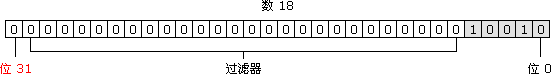
\includegraphics[scale=0.5]{js_integer_binary_signed_32bits.png}
\caption{ECMAScript 整数表示法}
\label{js_integer_binary_signed_32bits}
\end{figure}

18 的二进制版本只用了前 5 位,它们是这个数字的有效位。把数字转换成二进制字符串,就能看到有效位:


\begin{lstlisting}[language=JavaScript]
var iNum = 18;
alert(iNum.toString(2));	//输出 "10010"
\end{lstlisting}

这段代码只输出 "10010",而不是 18 的 32 位表示。其他的数位并不重要,因为仅使用前 5 位即可确定这个十进制数值。如下图所示:

\begin{figure}[!h]
\centering
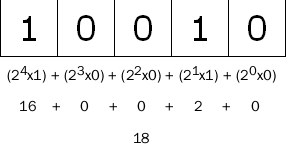
\includegraphics[scale=0.45]{js_integer_binary_number18.png}
\caption{18 的 32 位表示}
\label{js_integer_binary_number18}
\end{figure}


负数也存储为二进制代码,不过采用的形式是二进制补码。计算数字二进制补码的步骤有三步:

\begin{compactenum}
\item 确定该数字的非负版本的二进制表示(例如,要计算 -18的二进制补码,首先要确定 18 的二进制表示)
\item 求得二进制反码,即要把 0 替换为 1,把 1 替换为 0
\item 在二进制反码上加 1
\end{compactenum}

要确定 -18 的二进制表示,首先必须得到 18 的二进制表示,如下所示:

\verb|0000 0000 0000 0000 0000 0000 0001 0010|

接下来,计算二进制反码,如下所示:

\verb|1111 1111 1111 1111 1111 1111 1110 1101|

最后,在二进制反码上加 1,如下所示:

\begin{verbatim}
    1111 1111 1111 1111 1111 1111 1110 1101
                                          1
    ---------------------------------------
    1111 1111 1111 1111 1111 1111 1110 1110
\end{verbatim}

因此,-18 的二进制表示即\verb|1111 1111 1111 1111 1111 1111 1110 1110|。记住,在处理有符号整数时,开发者不能访问 31 位。

把负整数转换成二进制字符串后,ECMAScript 并不以二进制补码的形式显示,而是用数字绝对值的标准二进制代码前面加负号的形式输出。例如:

\begin{lstlisting}[language=JavaScript]
var iNum = -18;
alert(iNum.toString(2));	//输出 "-10010"
\end{lstlisting}

这段代码输出的是 "-10010",而非二进制补码,这是为避免访问位 31。为了简便,ECMAScript 用一种简单的方式处理整数,使得开发者不必关心它们的用法。

另一方面,无符号整数把最后一位作为另一个数位处理。在这种模式中,第 32 位不表示数字的符号,而是值 231。由于这个额外的位,无符号整数的数值范围为 0 到 4294967295。对于小于 2147483647 的整数来说,无符号整数看来与有符号整数一样,而大于 2147483647 的整数则要使用位 31(在有符号整数中,这一位总是 0)。

把无符号整数转换成字符串后,只返回它们的有效位。注意,所有整数字面量都默认存储为有符号整数,只有 ECMAScript 的位运算符才能创建无符号整数。

\section{NOT}

位运算 NOT 由否定号(~)表示,它是 ECMAScript 中为数不多的与二进制算术有关的运算符之一。

位运算 NOT 是三步的处理过程:

\begin{compactenum}
\item 把运算数转换成 32 位数字
\item 把二进制数转换成它的二进制反码
\item 把二进制数转换成浮点数
\end{compactenum}



\begin{lstlisting}[language=JavaScript]
var iNum1 = 25;		//25 等于 00000000000000000000000000011001
var iNum2 = ~iNum1;	//转换为 11111111111111111111111111100110
alert(iNum2);		//输出 "-26"
\end{lstlisting}

位运算 NOT 实质上是对数字求负,然后减 1,因此 25 变 -26。用下面的方法也可以得到同样的方法:


\begin{lstlisting}[language=JavaScript]
var iNum1 = 25;
var iNum2 = -iNum1 -1;
alert(iNum2);	//输出 -26
\end{lstlisting}



\section{AND}

位运算 AND 由和号(\&)表示,直接对数字的二进制形式进行运算。它把每个数字中的数位对齐,然后用下面的规则对同一位置上的两个数位进行 AND 运算:

\begin{longtable}{|m{120pt}|m{120pt}|m{120pt}|}
%head
\multicolumn{3}{r}{}
\tabularnewline\hline
第一个数字中的数位	&第二个数字中的数位	&结果
\endhead
%endhead

%firsthead
\hline
第一个数字中的数位	&第二个数字中的数位	&结果
\endfirsthead
%endfirsthead

%foot
\multicolumn{3}{r}{}
\endfoot
%endfoot


%lastfoot
\endlastfoot
%endlastfoot
\hline
1	&1	&1\\
\hline
1	&0	&0\\
\hline
0	&1	&0\\
\hline
0	&0	&0\\
\hline
\end{longtable}


例如,要对数字 25 和 3 进行 AND 运算,代码如下所示:

\begin{lstlisting}[language=JavaScript]
var iResult = 25 & 3;
alert(iResult);	//输出 "1"
\end{lstlisting}

25 和 3 进行 AND 运算的结果是 1。为什么?分析如下:

\begin{verbatim}
     25 = 0000 0000 0000 0000 0000 0000 0001 1001
      3 = 0000 0000 0000 0000 0000 0000 0000 0011
    ---------------------------------------------
    AND = 0000 0000 0000 0000 0000 0000 0000 0001
\end{verbatim}

可以看出,在 25 和 3 中,只有一个数位(位 0)存放的都是 1,因此,其他数位生成的都是 0,所以结果为 1。



\section{OR}

位运算 OR 由符号(|)表示,也是直接对数字的二进制形式进行运算。在计算每位时,OR 运算符采用下列规则:


\begin{longtable}{|m{120pt}|m{120pt}|m{120pt}|}
%head
\multicolumn{3}{r}{}
\tabularnewline\hline
第一个数字中的数位	&第二个数字中的数位	&结果
\endhead
%endhead

%firsthead
\hline
第一个数字中的数位	&第二个数字中的数位	&结果
\endfirsthead
%endfirsthead

%foot
\multicolumn{3}{r}{}
\endfoot
%endfoot


%lastfoot
\endlastfoot
%endlastfoot
\hline
1	&1	&1\\
\hline
1	&0	&1\\
\hline
0	&1	&1\\
\hline
0	&0	&0\\
\hline
\end{longtable}


仍然使用 AND 运算符所用的例子,对 25 和 3 进行 OR 运算,代码如下:


\begin{lstlisting}[language=JavaScript]
var iResult = 25 | 3;
alert(iResult);	//输出 "27"
\end{lstlisting}



25 和 3 进行 OR 运算的结果是 27:

\begin{verbatim}
    25 = 0000 0000 0000 0000 0000 0000 0001 1001
     3 = 0000 0000 0000 0000 0000 0000 0000 0011
    --------------------------------------------
    OR = 0000 0000 0000 0000 0000 0000 0001 1011
\end{verbatim}

可以看出,在两个数字中,共有 4 个数位存放的是 1,这些数位被传递给结果。二进制代码 11011 等于 27。



\section{XOR}


位运算 XOR 由符号(\^{})表示,当然,也是直接对二进制形式进行运算。XOR 不同于 OR,当只有一个数位存放的是 1 时,它才返回 1。真值表如下:


\begin{longtable}{|m{120pt}|m{120pt}|m{120pt}|}
%head
\multicolumn{3}{r}{}
\tabularnewline\hline
第一个数字中的数位	&第二个数字中的数位	&结果
\endhead
%endhead

%firsthead
\hline
第一个数字中的数位	&第二个数字中的数位	&结果
\endfirsthead
%endfirsthead

%foot
\multicolumn{3}{r}{}
\endfoot
%endfoot


%lastfoot
\endlastfoot
%endlastfoot
\hline
1	&1	&0\\
\hline
1	&0	&1\\
\hline
0	&1	&1\\
\hline
0	&0	&0\\
\hline
\end{longtable}

对 25 和 3 进行 XOR 运算,代码如下:

\begin{lstlisting}[language=JavaScript]
var iResult = 25 ^ 3;
alert(iResult);	//输出 "26"
\end{lstlisting}

25 和 3 进行 XOR 运算的结果是 26:

\begin{verbatim}
     25 = 0000 0000 0000 0000 0000 0000 0001 1001
      3 = 0000 0000 0000 0000 0000 0000 0000 0011
    ---------------------------------------------
    XOR = 0000 0000 0000 0000 0000 0000 0001 1010
\end{verbatim}

可以看出,在两个数字中,共有 4 个数位存放的是 1,这些数位被传递给结果。二进制代码 11010 等于 26。




\section{Left Shift Operator}



左移运算由两个小于号表示(<\/<)。它把数字中的所有数位向左移动指定的数量。例如,把数字 2(等于二进制中的 10)左移 5 位,结果为 64(等于二进制中的 1000000):

\begin{lstlisting}[language=JavaScript]
var iOld = 2;		//等于二进制 10
var iNew = iOld << 5;	//等于二进制 1000000 十进制 64
\end{lstlisting}

注意:在左移数位时,数字右边多出 5 个空位。左移运算用 0 填充这些空位,使结果成为完整的 32 位数字。

\begin{figure}[!h]
\centering
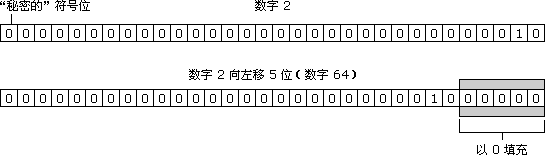
\includegraphics[scale=0.5]{js_operators_bitwise_leftshift.png}
\caption{左移运算}
\label{js_operators_bitwise_leftshift}
\end{figure}

注意:左移运算保留数字的符号位。例如,如果把 -2 左移 5 位,得到的是 -64,而不是 64。“符号仍然存储在第 32 位中吗?”是的,不过这在 ECMAScript 后台进行,开发者不能直接访问第 32 个数位。即使输出二进制字符串形式的负数,显示的也是负号形式(例如,-2 将显示 -10。)






\section{Signed right shift operator}


有符号右移运算符由两个大于号表示(>\/>)。它把 32 位数字中的所有数位整体右移,同时保留该数的符号(正号或负号)。有符号右移运算符恰好与左移运算相反。例如,把 64 右移 5 位,将变为 2:

\begin{lstlisting}[language=JavaScript]
var iOld = 64;		//等于二进制 1000000
var iNew = iOld >> 5;	//等于二进制 10 十进制 2
\end{lstlisting}


同样,移动数位后会造成空位。这次,空位位于数字的左侧,但位于符号位之后。ECMAScript 用符号位的值填充这些空位,创建完整的数字,如下图所示:

\begin{figure}[!h]
\centering
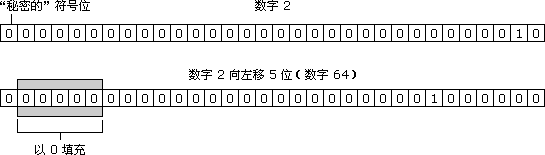
\includegraphics[scale=0.5]{js_operators_bitwise_signedrightshift.png}
\caption{有符号右移运算}
\label{js_operators_bitwise_signedrightshift}
\end{figure}





\section{Unsigned right shift operator}

无符号右移运算符由三个大于号(>\/>\/>)表示,它将无符号 32 位数的所有数位整体右移。对于正数,无符号右移运算的结果与有符号右移运算一样。


用有符号右移运算中的例子,把 64 右移 5 位,将变为 2:

\begin{lstlisting}[language=JavaScript]
var iOld = 64;		//等于二进制 1000000
var iNew = iOld >>> 5;	//等于二进制 10 十进制 2
\end{lstlisting}

对于负数,情况就不同了。

无符号右移运算用 0 填充所有空位。对于正数,这与有符号右移运算的操作一样,而负数则被作为正数来处理。

由于无符号右移运算的结果是一个 32 位的正数,所以负数的无符号右移运算得到的总是一个非常大的数字。例如,如果把 -64 右移 5 位,将得到 134217726。

要实现这一点,需要把这个数字转换成无符号的等价形式(尽管该数字本身还是有符号的),可以通过以下代码获得这种形式:

\begin{lstlisting}[language=JavaScript]
var iUnsigned64 = -64 >>> 0;
\end{lstlisting}

然后,用 Number 类型的 toString() 获取它的真正的位表示,采用的基为 2:


\begin{lstlisting}[language=JavaScript]
alert(iUnsigned64.toString(2));
\end{lstlisting}

这将生成 11111111111111111111111111000000,即有符号整数 -64 的二进制补码表示,不过它等于无符号整数 4294967232。

出于这种原因,使用无符号右移运算符要小心。

\chapter{Boolean Operators}


Boolean 运算符有三种:NOT、AND 和 OR,Boolean 运算符非常重要,它使得程序语言得以正常运行。


ECMAScript-262 v5 规范中描述的 ToBoolean 操作将其参数按照下表中的规则转换为逻辑值:

\begin{longtable}{|m{80pt}|m{280pt}|}
%head
\multicolumn{2}{r}{}
\tabularnewline\hline
参数类型	&结果
\endhead
%endhead

%firsthead
\caption{ECMAScript-262 v5 规范中描述的 ToBoolean 操作}\\
\hline
参数类型	&结果
\endfirsthead
%endfirsthead

%foot
\multicolumn{2}{r}{}
\endfoot
%endfoot


%lastfoot
\endlastfoot
%endlastfoot
\hline
Undefined	&false\\
\hline
Null		&false\\
\hline
Boolean		&结果等于输入的参数(不转换)\\
\hline
Number		&如果参数为 +0, -0 或 NaN,则结果为 false;否则为 true。\\
\hline
String		&如果参数为空字符串,则结果为 false;否则为 true。\\
\hline
Object		&true\\
\hline

\end{longtable}



\section{Logical NOT Operator}

在 ECMAScript 中,逻辑 NOT 运算符与 C 和 Java 中的逻辑 NOT 运算符相同,都由感叹号(!)表示。

与逻辑 OR 和逻辑 AND 运算符不同的是,逻辑 NOT 运算符返回的一定是 Boolean 值。

逻辑 NOT 运算符的行为如下:

\begin{compactitem}
\item 如果运算数是对象,返回 false
\item 如果运算数是数字 0,返回 true
\item 如果运算数是 0 以外的任何数字,返回 false
\item 如果运算数是 null,返回 true
\item 如果运算数是 NaN,返回 true
\item 如果运算数是 undefined,发生错误
\end{compactitem}


通常,该运算符用于控制循环:

\begin{lstlisting}[language=JavaScript]
var bFound = false;
var i = 0;

while (!bFound) {
  if (aValue[i] == vSearchValues) {
    bFound = true;
  } else {
    i++;
  }
}
\end{lstlisting}

在这个例子中,Boolean 变量(bFound)用于记录检索是否成功。找到问题中的数据项时,bFound 将被设置为 true,!bFound 将等于 false,意味着运行将跳出 while 循环。


判断 ECMAScript 变量的 Boolean 值时,也可以使用逻辑 NOT 运算符。这样做需要在一行代码中使用两个 NOT 运算符。无论运算数是什么类型,第一个 NOT 运算符返回 Boolean 值。第二个 NOT 将对该 Boolean 值求负,从而给出变量真正的 Boolean 值。

\begin{lstlisting}[language=JavaScript]
var bFalse = false;
var sRed = "red";
var iZero = 0;
var iThreeFourFive = 345;
var oObject = new Object;

document.write("bFalse 的逻辑值是 " + (!!bFalse));
document.write("sRed 的逻辑值是 " + (!!sRed));
document.write("iZero 的逻辑值是 " + (!!iZero));
document.write("iThreeFourFive 的逻辑值是 " + (!!iThreeFourFive));
document.write("oObject 的逻辑值是 " + (!!oObject));
\end{lstlisting}


结果如下:

\begin{lstlisting}[language=bash]
bFalse 的逻辑值是 false
sRed 的逻辑值是 true
iZero 的逻辑值是 false
iThreeFourFive 的逻辑值是 true
oObject 的逻辑值是 true 
\end{lstlisting}




\section{Logical AND Operator}

在 ECMAScript 中,逻辑 AND 运算符用双和号(\&\&)表示:

\begin{lstlisting}[language=JavaScript]
var bTrue = true;
var bFalse = false;
var bResult = bTrue && bFalse;
\end{lstlisting}

下面的真值表描述了逻辑 AND 运算符的行为:

\begin{longtable}{|m{120pt}|m{120pt}|m{120pt}|}
%head
\multicolumn{3}{r}{}
\tabularnewline\hline
运算数 1	&运算数 2	&结果
\endhead
%endhead

%firsthead
\caption{逻辑 AND 运算符}\\
\hline
运算数 1	&运算数 2	&结果
\endfirsthead
%endfirsthead

%foot
\multicolumn{3}{r}{}
\endfoot
%endfoot


%lastfoot
\endlastfoot
%endlastfoot
\hline
true	&true	&true\\
\hline
true	&false	&false\\
\hline
false	&true	&false\\
\hline
false	&false	&false\\
\hline
\end{longtable}

逻辑 AND 运算的运算数可以是任何类型的,不止是 Boolean 值。

如果某个运算数不是原始的 Boolean 型值,逻辑 AND 运算并不一定返回 Boolean 值:

\begin{compactitem}
\item 如果一个运算数是对象,另一个是 Boolean 值,返回该对象。
\item 如果两个运算数都是对象,返回第二个对象。
\item 如果某个运算数是 null,返回 null。
\item 如果某个运算数是 NaN,返回 NaN。
\item 如果某个运算数是 undefined,发生错误。
\end{compactitem}

与 Java 中的逻辑 AND 运算相似,ECMAScript 中的逻辑 AND 运算也是简便运算,即如果第一个运算数决定了结果,就不再计算第二个运算数。对于逻辑 AND 运算来说,如果第一个运算数是 false,那么无论第二个运算数的值是什么,结果都不可能等于 true。

考虑下面的例子:

\begin{lstlisting}[language=JavaScript]
var bTrue = true;
var bResult = (bTrue && bUnknown);	//发生错误
alert(bResult);			//这一行不会执行
\end{lstlisting}

这段代码在进行逻辑 AND 运算时将引发错误,因为变量 bUnknown 是未定义的。变量 bTrue 的值为 true,因为逻辑 AND 运算将继续计算变量 bUnknown。这样做就会引发错误,因为 bUnknown 的值是 undefined,不能用于逻辑 AND 运算。

如果修改这个例子,把第一个数设为 false,那么就不会发生错误:


\begin{lstlisting}[language=JavaScript]
var bFalse = false;
var bResult = (bFalse && bUnknown);
alert(bResult);			//输出 "false"
\end{lstlisting}

在这段代码中,脚本将输出逻辑 AND 运算返回的值,即字符串 "false"。即使变量 bUnknown 的值为 undefined,它也不会被计算,因为第一个运算数的值是 false。在使用逻辑 AND 运算符时,必须记住它的这种简便计算特性。




\section{Logical OR Operator}


ECMAScript 中的逻辑 OR 运算符与 Java 中的相同,都由双竖线(||)表示:


\begin{lstlisting}[language=JavaScript]
var bTrue = true;
var bFalse = false;
var bResult = bTrue || bFalse;
\end{lstlisting}


下面的真值表描述了逻辑 OR 运算符的行为:


\begin{longtable}{|m{120pt}|m{120pt}|m{120pt}|}
%head
\multicolumn{3}{r}{}
\tabularnewline\hline
运算数 1	&运算数 2	&结果
\endhead
%endhead

%firsthead
\caption{逻辑 OR 运算符}\\
\hline
运算数 1	&运算数 2	&结果
\endfirsthead
%endfirsthead

%foot
\multicolumn{3}{r}{}
\endfoot
%endfoot


%lastfoot
\endlastfoot
%endlastfoot
\hline
true	&true	&true\\
\hline
true	&false	&true\\
\hline
false	&true	&true\\
\hline
false	&false	&false\\
\hline
\end{longtable}

与逻辑 AND 运算符相似,如果某个运算数不是 Boolean 值,逻辑 OR 运算并不一定返回 Boolean 值:

\begin{compactitem}
\item 如果一个运算数是对象,并且该对象左边的运算数值均为 false,则返回该对象。
\item 如果两个运算数都是对象,返回第一个对象。
\item 如果最后一个运算数是 null,并且其他运算数值均为 false,则返回 null。
\item 如果最后一个运算数是 NaN,并且其他运算数值均为 false,则返回 NaN。
\item 如果某个运算数是 undefined,发生错误。
\end{compactitem}

与逻辑 AND 运算符一样,逻辑 OR 运算也是简便运算。对于逻辑 OR 运算符来说,如果第一个运算数值为 true,就不再计算第二个运算数。

\begin{lstlisting}[language=JavaScript]
var bTrue = true;
var bResult = (bTrue || bUnknown);
alert(bResult);			//输出 "true"
\end{lstlisting}

与前面的例子相同,变量 bUnknown 是未定义的。不过,由于变量 bTrue 的值为 true,bUnknown 不会被计算,因此输出的是 "true"。

如果把 bTrue 改为 false,将发生错误:

\begin{lstlisting}[language=JavaScript]
var bFalse = false;
var bResult = (bFalse || bUnknown);	//发生错误
alert(bResult);			//不会执行这一行
\end{lstlisting}



\chapter{Multiplicative Operators}



ECMAScript 的乘性运算符与 Java、C、Perl 等于语言中的同类运算符的运算方式相似。不过需要注意的是,乘性运算符还具有一些自动转换功能。



\section{Multiplication operator}

乘法运算符由星号(*)表示,用于两数相乘。ECMAScript 中的乘法语法与 C 语言中的相同:


\begin{lstlisting}[language=JavaScript]
var iResult = 12 * 34
\end{lstlisting}

不过,在处理特殊值时,ECMAScript 中的乘法还有一些特殊行为:


\begin{compactitem}
\item 如果结果太大或太小,那么生成的结果是 Infinity 或 -Infinity。
\item 如果某个运算数是 NaN,结果为 NaN。
\item Infinity 乘以 0,结果为 NaN。
\item Infinity 乘以 0 以外的任何数字,结果为 Infinity 或 -Infinity。
\item Infinity 乘以 Infinity,结果为 Infinity。
\end{compactitem}


如果运算数是数字,那么执行常规的乘法运算,即两个正数或两个负数为正数,两个运算数符号不同,结果为负数。



\section{Division operator}

除法运算符由斜杠(/)表示,用第二个运算数除第一个运算数:

\begin{lstlisting}[language=JavaScript]
var iResult = 88 /11;
\end{lstlisting}

与乘法运算符相似,在处理特殊值时,除法运算符也有一些特殊行为:

\begin{compactitem}
\item 如果结果太大或太小,那么生成的结果是 Infinity 或 -Infinity。
\item 如果某个运算数是 NaN,结果为 NaN。
\item Infinity 被 Infinity 除,结果为 NaN。
\item Infinity 被任何数字除,结果为 Infinity。
\item 0 除一个任何非无穷大的数字,结果为 NaN。
\item Infinity 被 0 以外的任何数字除,结果为 Infinity 或 -Infinity。
\end{compactitem}


如果运算数是数字,那么执行常规的除法运算,即两个正数或两个负数为正数,两个运算数符号不同,结果为负数。



\section{Modulo operator}

除法(余数)运算符由百分号(\%)表示,使用方法如下:


\begin{lstlisting}[language=JavaScript]
var iResult = 26%5; //等于 1
\end{lstlisting}

与其他乘性运算符相似,对于特殊值,取模运算符也有特殊的行为:

\begin{compactitem}
\item 如果被除数是 Infinity,或除数是 0,结果为 NaN。
\item Infinity 被 Infinity 除,结果为 NaN。
\item 如果除数是无穷大的数,结果为被除数。
\item 如果被除数为 0,结果为 0。
\end{compactitem}

如果运算数是数字,那么执行常规的算术除法运算,返回除法运算得到的余数。




\chapter{Additive Operators}


在多数程序设计语言中,加性运算符(即加号或减号)通常是最简单的数学运算符。在 ECMAScript 中,加性运算符有大量的特殊行为。

\section{Addition operator}

加法运算符由加号(+)表示:

\begin{lstlisting}[language=JavaScript]
var iResult = 1 + 2;
\end{lstlisting}

与乘性运算符一样,在处理特殊值时,ECMAScript 中的加法也有一些特殊行为:

\begin{compactitem}
\item 某个运算数是 NaN,那么结果为 NaN。
\item -Infinity 加 -Infinity,结果为 -Infinity。
\item Infinity 加 -Infinity,结果为 NaN。
\item +0 加 +0,结果为 +0。
\item -0 加 +0,结果为 +0。
\item -0 加 -0,结果为 -0。
\end{compactitem}

不过,如果某个运算数是字符串,那么采用下列规则:

\begin{compactitem}
\item 如果两个运算数都是字符串,把第二个字符串连接到第一个上。
\item 如果只有一个运算数是字符串,把另一个运算数转换成字符串,结果是两个字符串连接成的字符串。
\end{compactitem}

\begin{lstlisting}[language=JavaScript]
var result = 5 + 5;	//两个数字
alert(result);		//输出 "10"
var result2 = 5 + "5";	//一个数字和一个字符串
alert(result);		//输出 "55"
\end{lstlisting}

这段代码说明了加法运算符的两种模式之间的差别,即如果把数字与字符串相加,结果将成为字符串。


正常情况下,5+5 等于 10(原始数值),如上述代码中前两行所示。不过,如果把一个运算数改为字符串 "5",那么结果将变为 "55"(原始的字符串值),因为另一个运算数也会被转换为字符串。

JavaScript中的+ 运算符也可以用于把文本值或字符串变量加起来(连接起来),在使用加法运算符时,一定要仔细检查运算数的数据类型。

要想在两个字符串之间增加空格,就需要把空格插入一个字符串之中:

\begin{lstlisting}[language=JavaScript]
txt1="What a very ";
txt2="nice day";
txt3=txt1+txt2;
\end{lstlisting}

或者把空格插入表达式中:

\begin{lstlisting}[language=JavaScript]
txt1="What a very";
txt2="nice day";
txt3=txt1+" "+txt2;
\end{lstlisting}

在以上语句执行后,变量 txt3 包含的值是:\verb|"What a very nice day"|

\section{Subtraction operator}


减法运算符(-),也是一个常用的运算符:

\begin{lstlisting}[language=JavaScript]
var iResult = 2 - 1;
\end{lstlisting}


与加法运算符一样,在处理特殊值时,减法运算符也有一些特殊行为:

\begin{compactitem}
\item 某个运算数是 NaN,那么结果为 NaN。
\item Infinity 减 Infinity,结果为 NaN。
\item -Infinity 减 -Infinity,结果为 NaN。
\item Infinity 减 -Infinity,结果为 Infinity。
\item -Infinity 减 Infinity,结果为 -Infinity。
\item +0 减 +0,结果为 +0。
\item -0 减 -0,结果为 -0。
\item +0 减 -0,结果为 +0。
\item 某个运算符不是数字,那么结果为 NaN。
\end{compactitem}

如果运算数都是数字,那么执行常规的减法运算,并返回结果。





\chapter{Relational Operators}


关系运算符执行的是比较运算,每个关系运算符都返回一个布尔值。


关系运算符小于、大于、小于等于和大于等于执行的是两个数的比较运算,比较方式与算术比较运算相同,每个关系运算符都返回一个布尔值:

\begin{lstlisting}[language=JavaScript]
var bResult1 = 2 > 1	//true
var bResult2 = 2 < 1	//false
\end{lstlisting}

不过,对两个字符串应用关系运算符,它们的行为则不同。许多人认为小于表示“在字母顺序上靠前”,大于表示“在字母顺序上靠后”,但事实并非如此。

对于字符串,第一个字符串中每个字符的代码都与会第二个字符串中对应位置的字符的代码进行数值比较。完成这种比较操作后,返回一个 Boolean 值。问题在于大写字母的代码都小于小写字母的代码,这意味这着可能会遇到下列情况:


\begin{lstlisting}[language=JavaScript]
var bResult = "Blue" < "alpha";
alert(bResult);	//输出 true
\end{lstlisting}


在上面的例子中,字符串 "Blue" 小于 "alpha",因为字母 B 的字符代码是 66,字母 a 的字符代码是 97。要强制性得到按照真正的字母顺序比较的结果,必须把两个数转换成相同的大小写形式(全大写或全小写的),然后再进行比较:

\begin{lstlisting}[language=JavaScript]
var bResult = "Blue".toLowerCase() < "alpha".toLowerCase();
alert(bResult);	//输出 false
\end{lstlisting}


把两个运算数都转换成小写,确保了正确识别出 "alpha" 在字母顺序上位于 "Blue" 之前。

另一种棘手的状况发生在比较两个字符串形式的数字时,比如:


\begin{lstlisting}[language=JavaScript]
var bResult = "25" < "3";
alert(bResult);	//输出 "true"
\end{lstlisting}

上面这段代码比较的是字符串 "25" 和 "3"。两个运算数都是字符串,所以比较的是它们的字符代码("2" 的字符代码是 50,"3" 的字符代码是 51)。

不过,如果把某个运算数改为数字,那么结果如下:

\begin{lstlisting}[language=JavaScript]
var bResult = "25" < 3;
alert(bResult);	//输出 "false"
\end{lstlisting}




这里,字符串 "25" 将被转换成数字 25,然后与数字 3 进行比较,结果不出所料。

无论何时比较一个数字和一个字符串,ECMAScript 都会把字符串转换成数字,然后按照数字顺序比较它们。

不过,如果字符串不能转换成数字,首先考虑下面的例子:


\begin{lstlisting}[language=JavaScript]
var bResult = "a" < 3;
alert(bResult);
\end{lstlisting}

字母 "a" 不能转换成有意义的数字。不过,如果对它调用 parseInt() 方法,返回的是 NaN。根据规则,任何包含 NaN 的关系运算符都要返回 false,因此这段代码也输出 false。


通常,如果小于运算的两个值返回 false,那么大于等于运算必须返回 true,不过如果某个数字是 NaN,情况则非如此。


\chapter{Equal Operators}

判断两个变量是否相等是程序设计中非常重要的运算。在处理原始值时,这种运算相当简单,但涉及对象,任务就稍有点复杂。

ECMAScript 提供了两套等性运算符:等号和非等号用于处理原始值,全等号和非全等号用于处理对象。



\section{Equal sign \& Non-equal sign}

在 ECMAScript 中,等号由双等号(==)表示,当且仅当两个运算数相等时,它返回 true。非等号由感叹号加等号(!=)表示,当且仅当两个运算数不相等时,它返回 true。为确定两个运算数是否相等,这两个运算符都会进行类型转换。

执行类型转换的规则如下:


\begin{compactitem}
\item 如果一个运算数是 Boolean 值,在检查相等性之前,把它转换成数字值。false 转换成 0,true 为 1。
\item 如果一个运算数是字符串,另一个是数字,在检查相等性之前,要尝试把字符串转换成数字。
\item 如果一个运算数是对象,另一个是字符串,在检查相等性之前,要尝试把对象转换成字符串。
\item 如果一个运算数是对象,另一个是数字,在检查相等性之前,要尝试把对象转换成数字。
\end{compactitem}

在比较时,该运算符还遵守下列规则:

\begin{compactitem}
\item 值 null 和 undefined 相等。
\item 在检查相等性时,不能把 null 和 undefined 转换成其他值。
\item 如果某个运算数是 NaN,等号将返回 false,非等号将返回 true。
\item 如果两个运算数都是对象,那么比较的是它们的引用值。如果两个运算数指向同一对象,那么等号返回 true,否则两个运算数不等。
\end{compactitem}

即使两个数都是 NaN,等号仍然返回 false,因为根据规则,NaN 不等于 NaN。

下表列出了一些特殊情况,以及它们的结果:


\begin{longtable}{|m{140pt}|m{140pt}|}
%head
\multicolumn{2}{r}{}
\tabularnewline\hline
表达式	&值
\endhead
%endhead

%firsthead
\hline
表达式	&值
\endfirsthead
%endfirsthead

%foot
\multicolumn{2}{r}{}
\endfoot
%endfoot


%lastfoot
\endlastfoot
%endlastfoot
\hline
null == undefined	&true\\
\hline
"NaN" == NaN		&false\\
\hline
5 == NaN			&false\\
\hline
NaN == NaN		&false\\
\hline
NaN != NaN		&true\\
\hline
false == 0			&true\\
\hline
true == 1			&true\\
\hline
true == 2			&false\\
\hline
undefined == 0		&false\\
\hline
null == 0			&false\\
\hline
"5" == 5			&true\\
\hline
\end{longtable}



\section{Full equal sign\& Non-full Equal sign}



等号和非等号的同类运算符是全等号和非全等号。这两个运算符所做的与等号和非等号相同,只是它们在检查相等性前,不执行类型转换。

全等号由三个等号表示(===),只有在无需类型转换运算数就相等的情况下,才返回 true。


\begin{lstlisting}[language=JavaScript]
var sNum = "66";
var iNum = 66;
alert(sNum == iNum);	//输出 "true"
alert(sNum === iNum);	//输出 "false"
\end{lstlisting}

在这段代码中,第一个 alert 使用等号来比较字符串 "66" 和数字 66,输出 "true"。如前所述,这是因为字符串 "66" 将被转换成数字 66,,然后才与另一个数字 66 进行比较。第二个 alert 使用全等号在没有类型转换的情况下比较字符串和数字,当然,字符串不等于数字,所以输出 "false"。

非全等号由感叹号加两个等号(!==)表示,只有在无需类型转换运算数不相等的情况下,才返回 true。

\begin{lstlisting}[language=JavaScript]
var sNum = "66";
var iNum = 66;
alert(sNum != iNum);	//输出 "false"
alert(sNum !== iNum);	//输出 "true"
\end{lstlisting}


这里,第一个 alert 使用非等号,把字符串 "66" 转换成数字 66,使得它与第二个运算数 66 相等。因此,计算结果为 "false",因为两个运算数是相等的。第二个 alert 使用的非全等号。该运算是在问:"sNum" 与 "iNum" 不同吗?这个问题的答案是:是的(true),因为 sNum 是字符串,而 iNum 是数字,它们当然不同。





\chapter{Conditional Operators}

条件运算符是 ECMAScript 中功能最多的运算符,它的形式与 Java 中的相同。

\begin{lstlisting}[language=JavaScript]
variable = boolean_expression ? true_value : false_value;
\end{lstlisting}


该表达式主要是根据 boolean\_expression 的计算结果有条件地为变量赋值。如果 boolean\_expression 为 true,就把 true\_value 赋给变量;如果它是 false,就把 false\_value 赋给变量。


\begin{lstlisting}[language=JavaScript]
var iMax = (iNum1 > iNum2) ? iNum1 : iNum2;
\end{lstlisting}


在这里例子中,iMax 将被赋予数字中的最大值。表达式声明如果 iNum1 大于 iNum2,则把 iNum1 赋予 iMax。但如果表达式为 false(即 iNum2 大于或等于 iNum1),则把 iNum2 赋予 iMax。



\chapter{Assignment Operators}


简单的赋值运算符由等号(=)实现,只是把等号右边的值赋予等号左边的变量。


\begin{lstlisting}[language=JavaScript]
var iNum = 10;
\end{lstlisting}

复合赋值运算是由乘性运算符、加性运算符或位移运算符加等号(=)实现的。这些赋值运算符是下列这些常见情况的缩写形式:

\begin{lstlisting}[language=JavaScript]
var iNum = 10;
iNum = iNum + 10;
\end{lstlisting}

可以用一个复合赋值运算符改写第二行代码:

\begin{lstlisting}[language=JavaScript]
var iNum = 10;
iNum += 10;
\end{lstlisting}

每种主要的算术运算以及其他几个运算都有复合赋值运算符:

\begin{compactitem}
\item 乘法/赋值(*=)
\item 除法/赋值(/=)
\item 取模/赋值(\%=)
\item 加法/赋值(+=)
\item 减法/赋值(-=)
\item 左移/赋值(<\/<=)
\item 有符号右移/赋值(>\/>=)
\item 无符号右移/赋值(>\/>\/>=)
\end{compactitem}





\chapter{Comma Operators}

用逗号运算符可以在一条语句中执行多个运算。

\begin{lstlisting}[language=JavaScript]
var iNum1 = 1, iNum = 2, iNum3 = 3;
\end{lstlisting}

逗号运算符常用变量声明中。

\chapter{Summary of Operators}

\section{Arithmetic Operators}


JavaScrpt算术运算符用于执行变量与/或值之间的算术运算。

给定 y=5,下面的表格解释了这些算术运算符。

\begin{longtable}{|m{90pt}|m{90pt}|m{90pt}|m{90pt}|}
%head
\multicolumn{4}{r}{}
\tabularnewline\hline
运算符	&描述	&例子	&结果
\endhead
%endhead

%firsthead
\caption{JavaScript算术运算符}\\
\hline
运算符	&描述	&例子	&结果
\endfirsthead
%endfirsthead

%foot
\multicolumn{4}{r}{}
\endfoot
%endfoot

%lastfoot
\endlastfoot
%endlastfoot
\hline
+	&加					& x=y+2	&x=7\\
\hline
-	&减					& x=y-2	&x=3\\
\hline
*	&乘					& x=y*2	&x=10\\
\hline
/	&除					& x=y/2	&x=2.5\\
\hline
\%	&求余数 (保留整数)	&x=y\%2	&x=1\\
\hline
++	&累加				& x=++y	&x=6\\
\hline
--	&递减				& x=--y		& x=4\\
\hline


\end{longtable}


\section{Assignment Operators}


JavaScript赋值运算符用于给 JavaScript 变量赋值。

给定 x=10 和 y=5,下面的表格解释了赋值运算符。

\begin{longtable}{|m{90pt}|m{90pt}|m{90pt}|m{90pt}|}
%head
\multicolumn{4}{r}{}
\tabularnewline\hline
运算符	&例子	&等价于	&结果
\endhead
%endhead

%firsthead
\caption{JavaScript赋值运算符}\\
\hline
运算符	&例子	&等价于	&结果
\endfirsthead
%endfirsthead

%foot
\multicolumn{4}{r}{}
\endfoot
%endfoot

%lastfoot
\endlastfoot
%endlastfoot
\hline
=	&x=y	& 			& x=5\\
\hline
+=	&x+=y	&x=x+y	&x=15\\
\hline
-=	&x-=y	&x=x-y		& x=5\\
\hline
*=	&x*=y	&x=x*y		& x=50\\
\hline
/=	&x/=y	&x=x/y		& x=2\\
\hline
\%=	&x\%=y	&x=x\%y	& x=0\\
\hline

\end{longtable}





\section{Comparison Operators}

比较运算符在逻辑语句中使用,以测定变量或值是否相等。

给定 x=5,下面的表格解释了比较运算符。

\begin{longtable}{|m{120pt}|m{120pt}|m{120pt}|}
%head
\multicolumn{3}{r}{}
\tabularnewline\hline
运算符	&描述	&例子
\endhead
%endhead

%firsthead
\caption{JavaScript比较运算符}\\
\hline
运算符	&描述	&例子
\endfirsthead
%endfirsthead

%foot
\multicolumn{3}{r}{}
\endfoot
%endfoot

%lastfoot
\endlastfoot
%endlastfoot
\hline
=\/=		&等于				& x=\/=8 为 false\\
\hline
=\/=\/=		&全等(值和类型)	&x=\/=\/=5 为 true;x=\/=\/="5" 为 false\\
\hline
!\/=			&不等于			& x!\/=8 为 true\\
\hline
>			&大于				& x>8 为 false\\
\hline
<			&小于				& x<8 为 true\\
\hline
>\/=		&大于或等于		&x>\/=8 为 false\\
\hline
<\/=		&小于或等于		&x<\/=8 为 true\\
\hline
\end{longtable}

可以在条件语句中使用比较运算符对值进行比较,然后根据结果来采取行动:

\begin{lstlisting}[language=JavaScript]
if (age<18) document.write("Too young Too Simple");
if(age<=30&&age>18) document.write("图样图森破");
\end{lstlisting}



\section{Logical Operators}


逻辑运算符用于测定变量或值之间的逻辑。

给定 x=6 以及 y=3,下表解释了逻辑运算符。


\begin{longtable}{|m{120pt}|m{120pt}|m{120pt}|}
%head
\multicolumn{3}{r}{}
\tabularnewline\hline
运算符	&描述	&例子
\endhead
%endhead

%firsthead
\caption{JavaScript逻辑运算符}\\
\hline
运算符	&描述	&例子
\endfirsthead
%endfirsthead

%foot
\multicolumn{3}{r}{}
\endfoot
%endfoot

%lastfoot
\endlastfoot
%endlastfoot
\hline
\&\&	&and	&(x < 10 \&\& y > 1) 为 true\\
\hline
||		&or		& (x=\/=5 || y=\/=5) 为 false\\
\hline
!		&not	&!(x=\/=y) 为 true\\
\hline
\end{longtable}




\section{Conditional Operators}


JavaScript 还包含了基于某些条件对变量进行赋值的条件运算符。



\begin{lstlisting}[language=JavaScript]
variablename=(condition)?value1:value2 
\end{lstlisting}


要实现以下的条件判断并执行相应的代码,可以使用条件运算符。

如果变量 visitor 中的值是 "PRES",则向变量 greeting 赋值 "Dear President ",否则赋值 "Dear"。


\begin{lstlisting}[language=JavaScript]
greeting=(visitor=="PRES")?"Dear President ":"Dear ";
\end{lstlisting}












\part{Statements}


ECMA - 262 描述了 ECMAScript 的几种语句(statement),语句主要定义了 ECMAScript 的大部分语句,通常采用一个或多个关键字,完成给定的任务。

语句可以非常简单,例如通知函数退出,也可以非常复杂,如声明一组要反复执行的命令。


\chapter{If statements}

if 语句是 ECMAScript 中最常用的语句之一,事实上在许多计算机语言中都是如此。

if 语句的语法如下:

\begin{lstlisting}[language=JavaScript]
if (condition) statement1 else statement2
\end{lstlisting}

其中 condition 可以是任何表达式,计算的结果甚至不必是真正的 boolean 值,ECMAScript 会把它转换成 boolean 值。

如果条件计算结果为 true,则执行 statement1;如果条件计算结果为 false,则执行 statement2。

每个语句都可以是单行代码,也可以是代码块。

\begin{lstlisting}[language=JavaScript]
if (i > 30)
  {alert("大于 30");}
else
  {alert("小于等于 30");}
\end{lstlisting}

使用代码块被认为是一种最佳的编程实践,即使要执行的代码只有一行。这样做可以使每个条件要执行什么一目了然。

还可以串联多个 if 语句。就像这样:


\begin{lstlisting}[language=JavaScript]
if (condition1) statement1 else if (condition2) statement2 else statement3
\end{lstlisting}

例如:


\begin{lstlisting}[language=JavaScript]
if (i > 30) {
  alert("大于 30");
} else if (i < 0) {
  alert("小于 0");
} else {
  alert("在 0 到 30 之间");
}
\end{lstlisting}


\chapter{Iteration statements}


迭代语句又叫循环语句,声明一组要反复执行的命令,直到满足某些条件为止。循环通常用于迭代数组的值(因此而得名),或者执行重复的算术任务。

\section{do-while statements}

do-while 语句是后测试循环,即退出条件在执行循环内部的代码之后计算。这意味着在计算表达式之前,至少会执行循环主体一次。


它的语法如下:


\begin{lstlisting}[language=JavaScript]
do {statement} while (expression);
\end{lstlisting}

例子:

\begin{lstlisting}[language=JavaScript]
var i = 0;
do {i += 2;} while (i < 10);
\end{lstlisting}




\section{while statements}


while 语句是前测试循环。这意味着退出条件是在执行循环内部的代码之前计算的。因此,循环主体可能根本不被执行。


它的语法如下:

\begin{lstlisting}[language=JavaScript]
while (expression) statement
\end{lstlisting}


例子:

\begin{lstlisting}[language=JavaScript]
var i = 0;
while (i < 10) {
  i += 2;
}
\end{lstlisting}


\section{for statements}


for 语句是前测试循环,而且在进入循环之前,能够初始化变量,并定义循环后要执行的代码。


它的语法如下:

\begin{lstlisting}[language=JavaScript]
for (initialization; expression; post-loop-expression) statement
\end{lstlisting}

注意:post-loop-expression 之后不能写分号,否则无法运行。

例子:

\begin{lstlisting}[language=JavaScript]
iCount = 6;
for (var i = 0; i < iCount; i++) {
  alert(i);
}
\end{lstlisting}

这段代码定义了初始值为 0 的变量 i。只有当条件表达式(i < iCount)的值为 true 时,才进入 for 循环,这样循环主体可能不被执行。如果执行了循环主体,那么将执行循环后表达式,并迭代变量 i。

\section{for-in statements}


for 语句是严格的迭代语句,用于枚举对象的属性。

它的语法如下:


\begin{lstlisting}[language=JavaScript]
for (property in expression) statement
\end{lstlisting}

例子:


\begin{lstlisting}[language=JavaScript]
for (sProp in window) {
  alert(sProp);
}
\end{lstlisting}

这里,for-in 语句用于显示 window 对象的所有属性。

PropertyIsEnumerable() 是 ECMAScript 中专门用于说明属性是否可以用 for-in 语句访问的方法。

\chapter{Label statements}

可以用下列语句给语句加标签,以便以后调用:


\begin{lstlisting}[language=JavaScript]
label : statement
\end{lstlisting}

例如:

\begin{lstlisting}[language=JavaScript]
start : i = 5;
\end{lstlisting}

在这个例子中,标签 start 可以被之后的 break 或 continue 语句引用。




\chapter{Break \& Continue statements}


break 和 continue 语句对循环中的代码执行提供了更严格的控制。

break 和 continue 语句的不同之处在于,break 语句可以立即退出循环,阻止再次反复执行任何代码,而 continue 语句只是退出当前循环,根据控制表达式还允许继续进行下一次循环。


例如:

\begin{lstlisting}[language=JavaScript]
var iNum = 0;

for (var i=1; i<10; i++) {
  if (i % 5 == 0) {
    break;
  }
  iNum++;
}
alert(iNum);	//输出 "4"
\end{lstlisting}

在以上代码中,for 循环从 1 到 10 迭代变量 i。在循环主体中,if 语句将(使用取模运算符)检查 i 的值是否能被 5 整除。如果能被 5 整除,将执行 break 语句。alert 显示 "4",即退出循环前执行循环的次数。

如果用 continue 语句代替这个例子中的 break 语句,结果将不同:



\begin{lstlisting}[language=JavaScript]
var iNum = 0;

for (var i=1; i<10; i++) {
  if (i % 5 == 0) {
    continue;
  }
  iNum++;
}
alert(iNum);	//输出 "8"
\end{lstlisting}


这里,alert 将显示 "8",即执行循环的次数。可能执行的循环总数为 9,不过当 i 的值为 5 时,将执行 continue 语句,会使循环跳过表达式 iNum++,返回循环开头。

break 语句和 continue 语句都可以与有标签的语句联合使用,返回代码中的特定位置。

通常,当循环内部还有循环时,会这样做,例如:

\begin{lstlisting}[language=JavaScript]
var iNum = 0;

outermost:
for (var i=0; i<10; i++) {
  for (var j=0; j<10; j++) {
    if (i == 5 && j == 5) {
    break outermost;
  }
  iNum++;
  }
}

alert(iNum);	//输出 "55"
\end{lstlisting}


在上面的例子中,标签 outermost 表示的是第一个 for 语句。正常情况下,每个 for 语句执行 10 次代码块,这意味着 iNum++ 正常情况下将被执行 100 次,在执行完成时,iNum 应该等于 100。这里的 break 语句有一个参数,即停止循环后要跳转到的语句的标签。这样 break 语句不止能跳出内部 for 语句(即使用变量 j 的语句),还能跳出外部 for 语句(即使用变量 i 的语句)。因此,iNum 最后的值是 55,因为当 i 和 j 的值都等于 5 时,循环将终止。

可以以相同的方式使用 continue 语句:

\begin{lstlisting}[language=JavaScript]
var iNum = 0;

outermost:
for (var i=0; i<10; i++) {
  for (var j=0; j<10; j++) {
    if (i == 5 && j == 5) {
    continue outermost;
  }
  iNum++;
  }
}

alert(iNum);	//输出 "95"
\end{lstlisting}

在上例中,continue 语句会迫使循环继续,不止是内部循环,外部循环也如此。当 j 等于 5 时出现这种情况,意味着内部循环将减少 5 次迭代,致使 iNum 的值为 95。

可以看出,与 break 和 continue 联合使用的有标签语句非常强大,不过过度使用它们会给调试代码带来麻烦。要确保使用的标签具有说明性,同时不要嵌套太多层循环。








\chapter{With statements}


with 语句用于设置代码在特定对象中的作用域。

它的语法:

\begin{lstlisting}[language=JavaScript]
with (expression) statement
\end{lstlisting}

例如:

\begin{lstlisting}[language=JavaScript]
var sMessage = "hello";
with(sMessage) {
  alert(toUpperCase());	//输出 "HELLO"
}
\end{lstlisting}


在这个例子中,with 语句用于字符串,所以在调用 toUpperCase() 方法时,解释程序将检查该方法是否是本地函数。如果不是,它将检查伪对象 sMessage,看它是否为该对象的方法。然后,alert 输出 "HELLO",因为解释程序找到了字符串 "hello" 的 toUpperCase() 方法。

with 语句是运行缓慢的代码块,尤其是在已设置了属性值时。大多数情况下,如果可能,最好避免使用它。




\chapter{Switch statements}

switch 语句是 if 语句的兄弟语句,开发者可以用 switch 语句为表达式提供一系列的情况(case)。


switch 语句的语法如下:


\begin{lstlisting}[language=JavaScript]
switch (expression)
  case value: statement;
    break;
  case value: statement;
    break;
  case value: statement;
    break;
  case value: statement;
    break;
...
  case value: statement;
    break;
  default: statement;
\end{lstlisting}


每个情况(case)都是表示“如果 expression 等于 value,就执行 statement”。

关键字 break 会使代码跳出 switch 语句。如果没有关键字 break,代码执行就会继续进入下一个 case。

关键字 default 说明了表达式的结果不等于任何一种情况时的操作(事实上,它相对于 else 从句)。

switch 语句主要是为避免让开发者编写下面的代码:


\begin{lstlisting}[language=JavaScript]
if (i == 20)
  alert("20");
else if (i == 30)
  alert("30");
else if (i == 40)
  alert("40");
else
  alert("other");
\end{lstlisting}


等价的 switch 语句是这样的:


\begin{lstlisting}[language=JavaScript]
switch (i) {
  case 20: alert("20");
    break;
  case 30: alert("30");
    break;
  case 40: alert("40");
    break;
  default: alert("other");
}
\end{lstlisting}

ECMAScript 和 Java 中的 switch 语句有两点不同。在 ECMAScript 中,switch 语句可以用于字符串,而且能用不是常量的值说明情况:

\begin{lstlisting}[language=JavaScript]
var BLUE = "blue", RED = "red", GREEN  = "green";

switch (sColor) {
  case BLUE: alert("Blue");
    break;
  case RED: alert("Red");
    break;
  case GREEN: alert("Green");
    break;
  default: alert("Other");
}
\end{lstlisting}

这里,switch 语句用于字符串 sColor,声明 case 使用的是变量 BLUE、RED 和 GREEN,这在 ECMAScript 中是完全有效的。







\chapter{Recursion statements}

递归(英语:Recursion),又译为递回,在数学与计算机科学中,是指在函数的定义中使用函数自身的方法。递归一词还较常用于描述以自相似方法重复事物的过程。例如,当两面镜子相互之间近似平行时,镜中嵌套的图像是以无限递归的形式出现的。也可以理解为自我复制的过程。

\begin{figure}[!h]
\centering
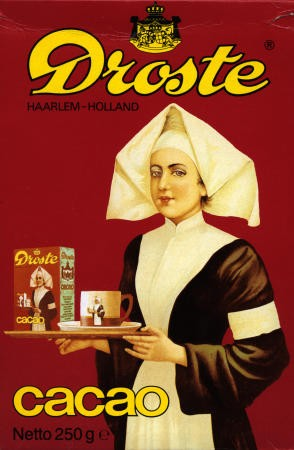
\includegraphics[scale=0.5]{Droste.jpg}
\caption{德罗斯特效应}
\label{Droste}
\end{figure}

德罗斯特效应是递归的一种视觉形式。图中女性手持的物体中有一幅她本人手持同一物体的小图片,进而小图片中还有更小的一幅她手持同一物体的图片,依此类推。


具体来说,递归(英语:recursion)在计算机科学中是指一种通过重复将问题分解为同类的子问题而解决问题的方法。递归式方法可以被用于解决很多的计算机科学问题,因此它是计算机科学中十分重要的一个概念。绝大多数编程语言支持函数的自调用,在这些语言中函数可以通过调用自身来进行递归。计算理论可以证明递归的作用可以完全取代循环,因此在很多函数编程语言(如Scheme)中习惯用递归来实现循环。

计算机科学家尼克劳斯·维尔特如此描述递归:

递归的强大之处在于它允许用户用有限的语句描述无限的对象。因此,在计算机科学中,递归可以被用来描述无限步的运算,尽管描述运算的程序是有限的。

\begin{flushright}
——尼克劳斯·维尔特
\end{flushright}



\section{Recursive functions and algorithms}


在支持自调用的编程语言中,递归可以通过简单的函数调用来完成,如计算阶乘的程序在数学上可以定义为:

\[\text{fact(n)}=\begin{cases}
1	\qquad \qquad \qquad\  \text{if n=0}\\
\text{n}\cdot \text{fact(n-1)} \qquad \text{if n>0}
\end{cases}\]

这一程序在Scheme语言中可以写作:

\begin{lstlisting}[language=Scheme]
(define (factorial n)
  (if (= n 0)
      1
      (* n (factorial (- n 1)))))
\end{lstlisting}



\section{Fixed-point combinator}


即使一个编程语言不支持自调用,如果在这语言中函数是第一类对象(即可以在运行期创建并作为变量处理),递归可以通过不动点组合子(英语:Fixed-point combinator)来产生。以下Scheme程序没有用到自调用,但是利用了一个叫做Z 算子(英语:Z combinator)的不动点组合子,因此同样能达到递归的目的。

\begin{lstlisting}[language=Scheme]
(define Z
  (lambda (f)
    ((lambda (recur) (f (lambda arg (apply (recur recur) arg))))
     (lambda (recur) (f (lambda arg (apply (recur recur) arg)))))))
 
(define fact
  (Z (lambda (f)
       (lambda (n)
         (if (<= n 0)
             1
             (* n (f (- n 1))))))))
\end{lstlisting}


这一程序思路是,既然在这里函数不能调用其自身,我们可以用 Z 组合子应用(application)这个函数后得到的函数再应用需计算的参数。

\section{Tail-recursive functions}


尾部递归是指递归函数在调用自身后直接传回其值,而不对其再加运算。尾部递归与循环是等价的,而且在一些语言(如Scheme中)可以被优化为循环指令。 因此,在这些语言中尾部递归不会占用调用堆栈空间。以下Scheme程序同样计算一个数字的阶乘,但是使用尾部递归:


\begin{lstlisting}[language=Scheme]
(define (factorial n)
  (define (iter product counter)
    (if (> counter n)
        product
        (iter (* counter product)
              (+ counter 1))))
  (iter 1 1))
\end{lstlisting}


\section{Recursive data types}



数据类型可以通过递归来进行定义,比如一个简单的递归定义为自然数的定义:“一个自然数或等于0,或等于另一个自然数加上1”。Haskell中可以定义链表为:



\begin{lstlisting}[language=Scheme]
data ListOfStrings = EmptyList | Cons String ListOfStrings
\end{lstlisting}

这一定义相当于声明“一个链表或是空串行,或是一个链表之前加上一个字符串”。可以看出所有链表都可以通过这一递归定义来达到。


\section{JavaScript Resurion Example}


需求:通过JavaScript实现让一个长60px,高30px的蓝色图块在5秒内移动200px。

HTML代码如下:




\begin{lstlisting}[language=HTML]
<!DOCTYPE html>
<html>
	<head>
		<link rel="stylesheet" type="text/css" href="animation.css">
		<title>js animation example</title>
	</head>
	<body>
		<div id="testdiv"></div>
		
		<script>
			var pos=document.getElementById("testdiv");
			var postyle = getComputedStyle(pos);
			var divleft =parseInt(postyle.marginLeft,10);
			
			function mvdiv(){	
				divleft+=2;
				mg=divleft+"px";
				//set testdiv new margin-left 
				pos.style.marginLeft=mg;

				//set animation length 200px
				//if length >=200, return
				if(divleft>=200)
					return

				//lanch 2px per 50 ms 
				setTimeout(mvdiv,50);
			}
			
			//lanch animation
			mvdiv();			

		</script>
	</body>
</html>
\end{lstlisting}

CSS代码如下:

\begin{lstlisting}[language=CSS]
#testdiv{
   margin-left:0px;
   height:30px;
   width:60px;
   background-color:#0000ff;
   position:static;
}
\end{lstlisting}






















\part{JavaScript Functions}

函数是一组可以随时随地运行的语句,而且函数是 ECMAScript 的核心。

函数是由这样的方式进行声明的:关键字 function、函数名、一组参数,以及置于括号中的待执行代码。

函数的基本语法是这样的:

\begin{lstlisting}[language=JavaScript]
function functionName(arg0, arg1, ... argN) {
  statements
}
\end{lstlisting}


例如:


\begin{lstlisting}[language=JavaScript]
function sayHi(sName, sMessage) {
  alert("Hello " + sName + sMessage);
}
\end{lstlisting}





函数可以通过其名字加上括号中的参数进行调用,如果有多个参数。

如果需要调用上例中的那个函数,可以使用如下的代码:

\begin{lstlisting}[language=JavaScript]
sayHi("David", " Nice to meet you!")
\end{lstlisting}


调用上面的函数 sayHi() 会生成一个警告窗口。

函数 sayHi() 未返回值,不过不必专门声明它(像在 Java 中使用 void 那样),而且即使函数确实有值,也不必明确地声明它。该函数只需要使用 return 运算符后跟要返回的值即可\footnote{如果函数无明确的返回值,或调用了没有参数的 return 语句,那么它真正返回的值是 undefined。}。


\begin{lstlisting}[language=JavaScript]
function sum(iNum1, iNum2) {
  return iNum1 + iNum2;
}
\end{lstlisting}

下面的代码把 sum 函数返回的值赋予一个变量:


\begin{lstlisting}[language=JavaScript]
var iResult = sum(1,1);
alert(iResult);	//输出 "2"
\end{lstlisting}

另一个重要概念是,与在 Java 中一样,函数在执行过 return 语句后立即停止代码。因此,return 语句后的代码都不会被执行。

例如,在下面的代码中,alert 窗口就不会显示出来:


\begin{lstlisting}[language=JavaScript]
function sum(iNum1, iNum2) {
  return iNum1 + iNum2;
  alert(iNum1 + iNum2);
}
\end{lstlisting}

一个函数中可以有多个 return 语句,如下所示:




\begin{lstlisting}[language=JavaScript]
function diff(iNum1, iNum2) {
  if (iNum1 > iNum2) {
    return iNum1 - iNum2;
  } else {
    return iNum2 - iNum1;
  }
}
\end{lstlisting}


上面的函数用于返回两个数的差。要实现这一点,必须用较大的数减去较小的数,因此用 if 语句决定执行哪个 return 语句。

如果函数无返回值,那么可以调用没有参数的 return 运算符,随时退出函数。

例如:

\begin{lstlisting}[language=JavaScript]
function sayHi(sMessage) {
  if (sMessage == "bye") {
    return;
  }
  alert(sMessage);
}
\end{lstlisting}


这段代码中,如果 sMessage 等于 "bye",就永远不显示警告框。


\chapter{arguments Object}


在函数代码中,使用特殊对象 arguments,开发者无需明确指出参数名,就能访问它们。

例如,在函数 sayHi() 中,第一个参数是 message。用 arguments[0] 也可以访问这个值,即第一个参数的值(第一个参数位于位置 0,第二个参数位于位置 1,依此类推)。因此,无需明确命名参数,就可以重写函数:


\begin{lstlisting}[language=JavaScript]
function sayHi() {
  if (arguments[0] == "bye") {
    return;
  }

  alert(arguments[0]);
}
\end{lstlisting}

还可以用 arguments 对象检测函数的参数个数,引用属性 arguments.length 即可。

下面的代码将输出每次调用函数使用的参数个数:

\begin{lstlisting}[language=JavaScript]
function howManyArgs() {
  alert(arguments.length);
}

howManyArgs("string", 45);
howManyArgs();
howManyArgs(12);
\end{lstlisting}


上面这段代码将依次显示 "2"、"0" 和 "1"。

与其他程序设计语言不同,ECMAScript 不会验证传递给函数的参数个数是否等于函数定义的参数个数。开发者定义的函数都可以接受任意个数的参数(根据 Netscape 的文档,最多可接受 25 个),而不会引发任何错误。任何遗漏的参数都会以 undefined 传递给函数,多余的函数将忽略。


用 arguments 对象判断传递给函数的参数个数,即可模拟函数重载:


\begin{lstlisting}[language=JavaScript]
function doAdd() {
  if(arguments.length == 1) {
    alert(arguments[0] + 5);
  } else if(arguments.length == 2) {
    alert(arguments[0] + arguments[1]);
  }
}

doAdd(10);	//输出 "15"
doAdd(40, 20);	//输出 "60"
\end{lstlisting}


当只有一个参数时,doAdd() 函数给参数加 5。如果有两个参数,则会把两个参数相加,返回它们的和。所以,doAdd(10) 输出的是 "15",而 doAdd(40, 20) 输出的是 "60"。

虽然不如重载那么好,不过已足以避开 ECMAScript 的这种限制。

\chapter{Function Object}



ECMAScript 的函数实际上就是功能完整的对象,Function 类可以表示开发者定义的任何函数。

用 Function 类直接创建函数的语法如下:

\begin{lstlisting}[language=JavaScript]
var function_name = new function(arg1, arg2, ..., argN, function_body)
\end{lstlisting}

在上面的形式中,每个 arg 都是一个参数,最后一个参数是函数主体(要执行的代码)。这些参数必须是字符串,示例代码如下:

\begin{lstlisting}[language=JavaScript]
var sayHi 
= 
new Function("sName", "sMessage", "alert(\"Hello \" + sName + sMessage);");
\end{lstlisting}

虽然由于字符串的关系,这种形式写起来有些困难,但有助于理解函数只不过是一种引用类型,它们的行为与用 Function 类明确创建的函数行为是相同的,所以上述代码等同于如下的函数定义:


\begin{lstlisting}[language=JavaScript]
function sayHi(sName, sMessage) {
  alert("Hello " + sName + sMessage);
}
\end{lstlisting}


参考下面的函数重载的示例:



\begin{lstlisting}[language=JavaScript]
function doAdd(iNum) {
  alert(iNum + 20);
}

function doAdd(iNum) {
  alert(iNum + 10);
}

doAdd(10);	//输出 "20"
\end{lstlisting}

这里,第二个函数重载了第一个函数,使 doAdd(10) 输出了 "20",而不是 "30"。如果以下面的形式重写该代码块,这个概念就清楚了:


\begin{lstlisting}[language=JavaScript]
var doAdd = new Function("iNum", "alert(iNum + 20)");
var doAdd = new Function("iNum", "alert(iNum + 10)");
doAdd(10);//输出“20”
\end{lstlisting}

很显然,doAdd 的值被改成了指向不同对象的指针,函数名只是指向函数对象的引用值,行为就像其他对象一样,甚至可以使两个变量指向同一个函数:



\begin{lstlisting}[language=JavaScript]
var doAdd = new Function("iNum", "alert(iNum + 10)");
var alsodoAdd = doAdd;
doAdd(10);	//输出 "20"
alsodoAdd(10);	//输出 "20"
\end{lstlisting}

在这里,变量 doAdd 被定义为函数,然后 alsodoAdd 被声明为指向同一个函数的指针。用这两个变量都可以执行该函数的代码,并输出相同的结果~——"20"。因此,如果函数名只是指向函数的变量,那么就可以把函数作为参数传递给另一个函数。


\begin{lstlisting}[language=JavaScript]
function callAnotherFunc(fnFunction, vArgument) {
  fnFunction(vArgument);
}

var doAdd = new Function("iNum", "alert(iNum + 10)");

callAnotherFunc(doAdd, 10);	//输出 "20"
\end{lstlisting}

在上面的例子中,callAnotherFunc() 有两个参数~——要调用的函数和传递给该函数的参数。这段代码把 doAdd() 传递给 callAnotherFunc() 函数,参数是 10,输出 "20"。

注意:尽管可以使用 Function 构造函数创建函数,但最好不要使用它,因为用它定义函数比用传统方式要慢得多。不过,所有函数都应看作 Function 类的实例。


\section{Function Object property}

函数属于引用类型,所以它们也有属性和方法。ECMAScript 定义的属性 length 声明了函数期望的参数个数。例如:


\begin{lstlisting}[language=JavaScript]
function doAdd(iNum) {
  alert(iNum + 10);
}

function sayHi() {
  alert("Hi");
}

alert(doAdd.length);	//输出 "1"
alert(sayHi.length);	//输出 "0"
\end{lstlisting}

函数 doAdd() 定义了一个参数,因此它的 length 是 1;sayHi() 没有定义参数,所以 length 是 0。

无论定义了几个参数,ECMAScript 可以接受任意多个参数(最多 25 个),属性 length 只是为查看默认情况下预期的参数个数提供了一种简便方式。




\section{Function Object method}

Function 对象也有与所有对象共享的 valueOf() 方法和 toString() 方法。这两个方法返回的都是函数的源代码,在调试时尤其有用。例如:

\begin{lstlisting}[language=JavaScript]
function doAdd(iNum) {
  alert(iNum + 10);
}

document.write(doAdd.toString());
\end{lstlisting}

上面这段代码输出了 doAdd() 函数的文本。

\chapter{closure}


闭包,指的是词法表示包括不被计算的变量的函数,也就是说,函数可以使用函数之外定义的变量。


ECMAScript 最易让人误解的一点是,它支持闭包(closure)。

在 ECMAScript 中使用全局变量是一个简单的闭包实例,思考下面这段代码:

\begin{lstlisting}[language=JavaScript]
var sMessage = "hello world";

function sayHelloWorld() {
  alert(sMessage);
}

sayHelloWorld();
\end{lstlisting}


在上面这段代码中,脚本被载入内存后,并没有为函数 sayHelloWorld() 计算变量 sMessage 的值。该函数捕获 sMessage 的值只是为了以后的使用,也就是说,解释程序知道在调用该函数时要检查 sMessage 的值。sMessage 将在函数调用 sayHelloWorld() 时(最后一行)被赋值,显示消息 "hello world"。

在一个函数中定义函数另一个会使闭包变得更加复杂。例如:



\begin{lstlisting}[language=JavaScript]
var iBaseNum = 10;

function addNum(iNum1, iNum2) {
  function doAdd() {
    return iNum1 + iNum2 + iBaseNum;
  }
  return doAdd();
}
\end{lstlisting}


这里,函数 addNum() 包括函数 doAdd() (闭包)。内部函数是一个闭包,因为它将获取外部函数的参数 iNum1 和 iNum2 以及全局变量 iBaseNum 的值。 addNum() 的最后一步调用了 doAdd(),把两个参数和全局变量相加,并返回它们的和。

这里要掌握的重要概念是,doAdd() 函数根本不接受参数,它使用的值是从执行环境中获取的。

可以看到,闭包是 ECMAScript 中非常强大多用的一部分,可用于执行复杂的计算。就像使用任何高级函数一样,使用闭包要小心,因为它们可能会变得非常复杂。


























\part{Regular Expression}


\part{Objects}


\begin{compactitem}
\item 对象

ECMA-262 把对象(object)定义为“属性的无序集合,每个属性存放一个原始值、对象或函数”。严格来说,这意味着对象是无特定顺序的值的数组。

尽管 ECMAScript 如此定义对象,但它更通用的定义是基于代码的名词(人、地点或事物)的表示。

\item 类

每个对象都由类定义,可以把类看做对象的配方。类不仅要定义对象的接口(interface)(开发者访问的属性和方法),还要定义对象的内部工作(使属性和方法发挥作用的代码)。编译器和解释程序都根据类的说明构建对象。


\item 实例

程序使用类创建对象时,生成的对象叫作类的实例(instance)。对类生成的对象的个数的唯一限制来自于运行代码的机器的物理内存。每个实例的行为相同,但实例处理一组独立的数据。由类创建对象实例的过程叫做实例化(instantiation)。

对象的创建和销毁都在 JavaScript 执行过程中发生,理解这种范式的含义对理解整个语言至关重要。


\end{compactitem}


ECMAScript 并没有正式的类,相反,ECMA-262 把对象定义描述为对象的配方,这是 ECMAScript 逻辑上的一种折中方案,因为对象定义实际上是对象自身。

在 ECMAScript 中,对象由特性(attribute)构成,特性可以是原始值,也可以是引用值。如果特性存放的是函数,它将被看作对象的方法(method),否则该特性被看作对象的属性(property)。

即使类并不真正存在,我们也把对象定义叫做类,因为大多数开发者对此术语更熟悉,而且从功能上说,两者是等价的。


一种面向对象语言需要向开发者提供四种基本能力:

\begin{compactenum}
\item 封装 - 把相关的信息(无论数据或方法)存储在对象中的能力
\item 聚集 - 把一个对象存储在另一个对象内的能力
\item 继承 - 由另一个类(或多个类)得来类的属性和方法的能力
\item 多态 - 编写能以多种方法运行的函数或方法的能力
\end{compactenum}

ECMAScript 支持这些要求,因此可被是看做面向对象的。


\chapter{Object declaration}








\chapter{Object instantiation}


对象的创建方式是用关键字 new 后面跟上实例化的类的名字:


\begin{lstlisting}[language=JavaScript]
var oObject = new Object();
var oStringObject = new String();
\end{lstlisting}

第一行代码创建了 Object 类的一个实例,并把它存储到变量 oObject 中。第二行代码创建了 String 类的一个实例,把它存储在变量 oStringObject 中。如果构造函数无参数,括号则不是必需的。因此可以采用下面的形式重写上面的两行代码:

\begin{lstlisting}[language=JavaScript]
var oObject = new Object;
var oStringObject = new String;
\end{lstlisting}


\chapter{Object reference}


在 ECMAScript 中,不能访问对象的物理表示,只能访问对象的引用。每次创建对象,存储在变量中的都是该对象的引用,而不是对象本身。



\chapter{Object dereference}

ECMAScript 拥有无用存储单元收集程序(garbage collection routine),意味着不必专门销毁对象来释放内存。当再没有对对象的引用时,称该对象被废除(dereference)了。运行无用存储单元收集程序时,所有废除的对象都被销毁。每当函数执行完它的代码,无用存储单元收集程序都会运行,释放所有的局部变量,还有在一些其他不可预知的情况下,无用存储单元收集程序也会运行。

把对象的所有引用都设置为 null,可以强制性地废除对象。例如:

\begin{lstlisting}[language=JavaScript]
var oObject = new Object;
// do something with the object here
oObject = null;
\end{lstlisting}


当变量 oObject 设置为 null 后,对第一个创建的对象的引用就不存在了。这意味着下次运行无用存储单元收集程序时,该对象将被销毁。

每用完一个对象后,就将其废除,来释放内存,这是个好习惯。这样还确保不再使用已经不能访问的对象,从而防止程序设计错误的出现。此外,旧的浏览器(如 IE/MAC)没有全面的无用存储单元收集程序,所以在卸载页面时,对象可能不能被正确销毁。废除对象和它的所有特性是确保内存使用正确的最好方法。

废除对象的所有引用时要当心。如果一个对象有两个或更多引用,则要正确废除该对象,必须将其所有引用都设置为 null。

\chapter{Object binding}


所谓绑定(binding),即把对象的接口与对象实例结合在一起的方法。

早绑定(early binding)是指在实例化对象之前定义它的属性和方法,这样编译器或解释程序就能够提前转换机器代码。在 Java 和 Visual Basic 这样的语言中,有了早绑定,就可以在开发环境中使用 IntelliSense(即给开发者提供对象中属性和方法列表的功能)。ECMAScript 不是强类型语言,所以不支持早绑定。

另一方面,晚绑定(late binding)指的是编译器或解释程序在运行前,不知道对象的类型。使用晚绑定,无需检查对象的类型,只需检查对象是否支持属性和方法即可。ECMAScript 中的所有变量都采用晚绑定方法,这样就允许执行大量的对象操作,而无任何惩罚。




\chapter{Object Types}

在 ECMAScript 中,所有对象并非同等创建的。一般来说,可以创建并使用的对象有三种:本地对象、内置对象和宿主对象。



\section{Native Objects}

ECMA-262 把本地对象(native object)定义为“独立于宿主环境的 ECMAScript 实现提供的对象”。简单来说,本地对象就是 ECMA-262 定义的类(引用类型)。它们包括:


\begin{compactitem}
\item Object
\item Function
\item Array
\item String
\item Boolean
\item Number
\item Date
\item RegExp
\item Error
\item EvalError
\item RangeError
\item ReferenceError
\item SyntaxError
\item TypeError
\item URIError
\end{compactitem}



\section{Build-in Objects}

ECMA-262 把内置对象(built-in object)定义为“由 ECMAScript 实现提供的、独立于宿主环境的所有对象,在 ECMAScript 程序开始执行时出现”。这意味着开发者不必明确实例化内置对象,它已被实例化了。

ECMA-262 只定义了两个内置对象,即 Global 和 Math (它们也是本地对象,根据定义,每个内置对象都是本地对象)。


\section{Host Objects}

所有非本地对象都是宿主对象(host object),即由 ECMAScript 实现的宿主环境提供的对象。
所有 BOM 和 DOM 对象都是宿主对象。


\chapter{Object scope}


作用域指的是变量的适用范围。

在传统的面向对象程序设计中,主要关注于公用和私有作用域。

\begin{compactitem}
\item 公用作用域(public scope)

公用作用域中的对象属性可以从对象外部访问,即开发者创建对象的实例后,就可使用它的公用属性。

\item 私有作用域(private scope)

私有作用域中的属性只能在对象内部访问,即对于外部世界来说,这些属性并不存在,这意味着如果类定义了私有属性和方法,则它的子类也不能访问这些属性和方法。
\item 受保护作用域(protected scope)

受保护作用域也是用于定义私有的属性和方法,只是这些属性和方法还能被其子类访问。

\end{compactitem}




\section{Object public scope}

ECMAScript 只有公用作用域。

对 ECMAScript 讨论上面这些作用域几乎毫无意义,因为 ECMAScript 中只存在一种作用域~——公用作用域。

ECMAScript 中的所有对象的所有属性和方法都是公用的,因此,定义自己的类和对象时,必须格外小心,因此所有属性和方法默认都是公用的。






\section{Object private scope}



ECMAScript 没有私有作用域。


不过,许多开发者都在网上提出了有效的属性作用域模式,解决了 ECMAScript 的这种问题。


\begin{lstlisting}[language=JavaScript]
obj._color_ = "blue";
\end{lstlisting}

这段代码中,属性 color 是私有的。注意,下划线并不改变属性是公用属性的事实,它只是告诉其他开发者,应该把该属性看作私有的。

当然,也有些开发者还喜欢用单下划线说明私有成员,例如:obj.\_color。


\section{Object protected scope}


ECMAScript 没有受保护作用域。




\section{Object static scope}

静态作用域定义的属性和方法任何时候都能从同一位置访问。在 Java 中,类可具有属性和方法,无需实例化该类的对象,即可访问这些属性和方法,例如 java.net.URLEncoder 类,它的函数 encode() 就是静态方法。

ECMAScript 没有静态作用域。

严格来说,ECMAScript 并没有静态作用域。不过,它可以给构造函数提供属性和方法。

构造函数只是函数,而函数是对象,对象可以有属性和方法。例如:



\begin{lstlisting}[language=JavaScript]
function sayHello() {
  alert("hello");
}

sayHello.alternate = function() {
  alert("hi");
}

sayHello();		//输出 "hello"
sayHello.alternate();	//输出 "hi"
\end{lstlisting}

这里,方法 alternate() 实际上是函数 sayHello 的方法。可以像调用常规函数一样调用 sayHello() 输出 "hello",也可以调用 sayHello.alternate() 输出 "hi"。即使如此,alternate() 也是 sayHello() 公用作用域中的方法,而不是静态方法。


\section{this}


在 ECMAScript 中,要掌握的最重要的概念之一是关键字 this 的用法,它用在对象的方法中。


关键字 this 总是指向调用该方法的对象,例如:


\begin{lstlisting}[language=JavaScript]
var oCar = new Object;
oCar.color = "red";
oCar.showColor = function() {
  alert(this.color);
};

oCar.showColor();		//输出 "red"
\end{lstlisting}

在上面的代码中,关键字 this 用在对象的 showColor() 方法中。在此环境中,this 等于 oCar。下面的代码与上面的代码的功能相同:

\begin{lstlisting}[language=JavaScript]
var oCar = new Object;
oCar.color = "red";
oCar.showColor = function() {
  alert(oCar.color);
};

oCar.showColor();		//输出 "red"
\end{lstlisting}



为什么使用 this 呢?因为在实例化对象时,总是不能确定开发者会使用什么样的变量名。使用 this,即可在任何多个地方重用同一个函数。思考下面的例子:


\begin{lstlisting}[language=JavaScript]
function showColor() {
  alert(this.color);
};

var oCar1 = new Object;
oCar1.color = "red";
oCar1.showColor = showColor;

var oCar2 = new Object;
oCar2.color = "blue";
oCar2.showColor = showColor;

oCar1.showColor();		//输出 "red"
oCar2.showColor();		//输出 "blue"
\end{lstlisting}


在上面的代码中,首先用 this 定义函数 showColor(),然后创建两个对象(oCar1 和 oCar2),一个对象的 color 属性被设置为 "red",另一个对象的 color 属性被设置为 "blue"。两个对象都被赋予了属性 showColor,指向原始的 showColor () 函数(注意这里不存在命名问题,因为一个是全局函数,而另一个是对象的属性)。调用每个对象的 showColor(),oCar1 输出是 "red",而 oCar2 的输出是 "blue"。这是因为调用 oCar1.showColor() 时,函数中的 this 关键字等于 oCar1。调用 oCar2.showColor() 时,函数中的 this 关键字等于 oCar2。


注意,引用对象的属性时,必须使用 this 关键字。例如,如果采用下面的代码,showColor() 方法不能运行:

\begin{lstlisting}[language=JavaScript]
function showColor() {
  alert(color);
};
\end{lstlisting}

如果不用对象或 this 关键字引用变量,ECMAScript 就会把它看作局部变量或全局变量。然后该函数将查找名为 color 的局部或全局变量,但是不会找到,这样该函数将在警告中显示 "null"。



\chapter{Object defination}


使用预定义对象只是面向对象语言的能力的一部分,它真正强大之处在于能够创建自己专用的类和对象。



ECMAScript 拥有很多创建对象或类的方法。





\section{factory function}


因为对象的属性可以在对象创建后动态定义,所有许多开发者都在 JavaScript 最初引入时编写类似下面的代码:

\begin{lstlisting}[language=JavaScript]
var oCar = new Object;
oCar.color = "blue";
oCar.doors = 4;
oCar.mpg = 25;
oCar.showColor = function() {
  alert(this.color);
};
\end{lstlisting}

在上面的代码中,创建对象 car,然后给它设置几个属性:它的颜色是蓝色,有四个门,每加仑油可以跑 25 英里。最后一个属性实际上是指向函数的指针,意味着该属性是个方法。执行这段代码后,就可以使用对象 car。

不过这里有一个问题,就是可能需要创建多个 car 的实例。

要解决该问题,开发者创造了能创建并返回特定类型的对象的工厂函数(factory function),例如,函数 createCar() 可用于封装前面列出的创建 car 对象的操作:

\begin{lstlisting}[language=JavaScript]
function createCar() {
  var oTempCar = new Object;
  oTempCar.color = "blue";
  oTempCar.doors = 4;
  oTempCar.mpg = 25;
  oTempCar.showColor = function() {
    alert(this.color);
  };
  return oTempCar;
}

var oCar1 = createCar();
var oCar2 = createCar();
\end{lstlisting}

在这里,第一个例子中的所有代码都包含在 createCar() 函数中。此外,还有一行额外的代码,返回 car 对象(oTempCar)作为函数值。调用此函数,将创建新对象,并赋予它所有必要的属性,复制出一个我们在前面说明过的 car 对象。因此,通过这种方法,我们可以很容易地创建 car 对象的两个版本(oCar1 和 oCar2),它们的属性完全一样。


我们还可以修改 createCar() 函数,给它传递各个属性的默认值,而不是简单地赋予属性默认值:



\begin{lstlisting}[language=JavaScript]
function createCar(sColor,iDoors,iMpg) {
  var oTempCar = new Object;
  oTempCar.color = sColor;
  oTempCar.doors = iDoors;
  oTempCar.mpg = iMpg;
  oTempCar.showColor = function() {
    alert(this.color);
  };
  return oTempCar;
}

var oCar1 = createCar("red",4,23);
var oCar2 = createCar("blue",3,25);

oCar1.showColor();		//输出 "red"
oCar2.showColor();		//输出 "blue"
\end{lstlisting}


给 createCar() 函数加上参数,即可为要创建的 car 对象的 color、doors 和 mpg 属性赋值,这使两个对象具有相同的属性,却有不同的属性值。


虽然 ECMAScript 越来越正式化,但创建对象的方法却被置之不理,且其规范化至今还遭人反对。一部分是语义上的原因(它看起来不像使用带有构造函数 new 运算符那么正规),一部分是功能上的原因。功能原因则在于用这种方式必须创建对象的方法。前面的例子中,每次调用函数 createCar(),都要创建新函数 showColor(),意味着每个对象都有自己的 showColor() 版本,而事实上,每个对象都共享同一个函数。

有些开发者在工厂函数外定义对象的方法,然后通过属性指向该方法,从而避免这个问题:


\begin{lstlisting}[language=JavaScript]
function createCar(sColor,iDoors,iMpg) {
  var oTempCar = new Object;
  oTempCar.color = sColor;
  oTempCar.doors = iDoors;
  oTempCar.mpg = iMpg;
  oTempCar.showColor = function() {
    alert(this.color);
  };
  return oTempCar;
}

var oCar1 = createCar("red",4,23);
var oCar2 = createCar("blue",3,25);

oCar1.showColor();		//输出 "red"
oCar2.showColor();		//输出 "blue"
\end{lstlisting}


在上面这段重写的代码中,在函数 createCar() 之前定义了函数 showColor()。在 createCar() 内部,赋予对象一个指向已经存在的 showColor() 函数的指针。从功能上讲,这样解决了重复创建函数对象的问题;但是从语义上讲,该函数不太像是对象的方法。

所有这些问题都引发了开发者定义的构造函数的出现。




\section{Constructor mode}


创建构造函数就像创建工厂函数一样容易。第一步选择类名,即构造函数的名字。根据惯例,这个名字的首字母大写,以使它与首字母通常是小写的变量名分开。除了这点不同,构造函数看起来很像工厂函数。考虑下面的例子:


\begin{lstlisting}[language=JavaScript]
function Car(sColor,iDoors,iMpg) {
  this.color = sColor;
  this.doors = iDoors;
  this.mpg = iMpg;
  this.showColor = function() {
    alert(this.color);
  };
}

var oCar1 = new Car("red",4,23);
var oCar2 = new Car("blue",3,25);
\end{lstlisting}






\section{Prototype mode}








\section{Mixed constructor / prototype}






\section{Dynamic Prototype}







\section{Mixed factory mode}






















































\part{Inheritance}



\end{document}












